% !TEX root = ../../Tesi_Triennale_PMNS.tex
\chapter{Analisi}
\label{chapter:analisi}
\begin{wrapfigure}{r}{0.4\textwidth}
	\vspace{-10pt}
	\begin{center}
		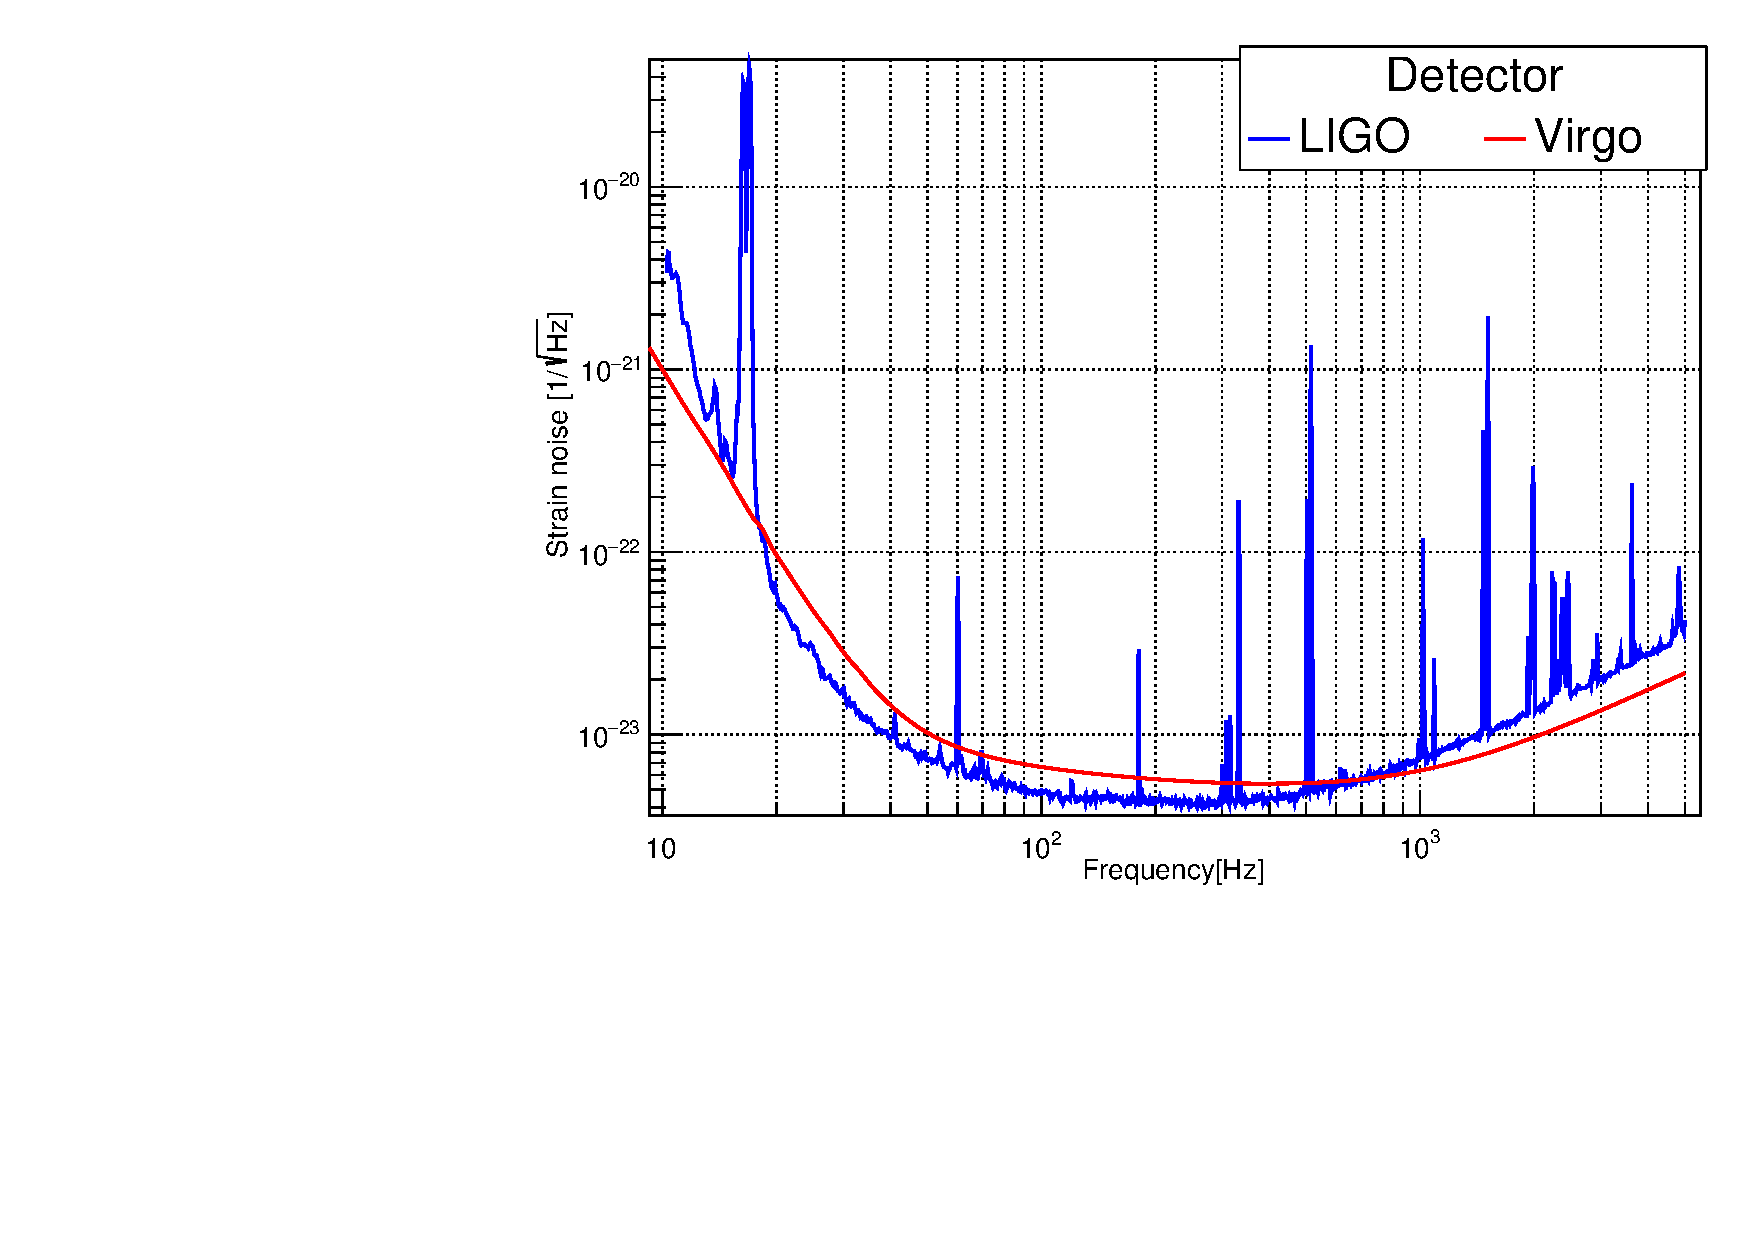
\includegraphics[width=0.4\textwidth]{figures/Capitolo_3/report/pds.pdf}
	\end{center}
	\vspace{-5pt}
	\caption{Sensibilità della rete}
	\label{fig:sensitivity_O4}
	\vspace{-10pt}
\end{wrapfigure}
Verranno riportati in questo capitolo i risultati di simulazioni effettuate iniettando i segnali in posizioni celesti generiche e ricostruite con cWB. Dopo aver mostrato preliminarmente la ricostruzione di un singolo evento simulato per descrivere i vantaggi e i limiti della ricostruzione con questo algoritmo, verranno riportati i risultati della campagna di simulazioni. In particolare verranno riportati i risultati di compatibilità delle forme d'onda ricostruite rispetto alle iniezioni fatte e verrà presentato un metodo per valutare una stima sistematica per la frequenza della post-coaelescenza.\\
Le analisi vengono effettuate simulando segnali sovrapposti ad un rumore gaussiano atteso per i rivelatori LIGO Livingstone, LIGO Hanford e Virgo nel run O4 come da curva di sensibilità riportata in Figura \ref{fig:sensitivity_O4}, non si considera invece il rivelatore Kagra, nonostante sia previsto si unisca alla rete di interferometri per la presa dati di O4. In particolare il run O4 è previsto avere una durata di un anno e i rivelatori utilizzati saranno i due interferometri LIGO con obiettivo di sensibilità per BNS nel range $160-190$Mpc, Virgo con sensiblità $90-120$Mpc e Kagra nel range $25-130$Mpc \cite{Abbott_2020a}. In particolare questa notazione per indicare la sensibilità del rivelatore indica la massima distanza rivelabile attesa per una misurazione con SNR di 8 della coalescenza di una coppia di stelle di neutroni di massa $\SI{1.4}{\solarmass}$ simulata in una posizione nel cielo causale (o per polarizzazione che massimizza snr). In questo run di misure è atteso un numero di rivelazioni di BNS di $10^{+52}_{-10}$ con risoluzione sulla posizione mediana di $33_{-5}^{+5}$deg$^2$ con intervallo di credibilità del 90\%\cite{Abbott_2020a}.\\
Le curve in figura sono stime intermedie per il run O4, quindi nella notazione precedente gli interferometri LIGO presentano sensibilità di 140Mpc, mentre il rivelatore Virgo di 100Mpc.
Si osserva che per i rivelatori LIGO-Hanford e LIGO-Livingstone le curve risultano ben caratterizzate avendo, oltre alla curva teorica, foreste di picchi frutto di risonanze e altri fenomeni che ne compromettono in parte la sensibilità; per Virgo invece si utilizza una curva semplificata, per cui la sensibilità risulterà generalmente sovrastimata rispetto ai risultati che si potranno ottenere nel run O4.\\
Si osserva inoltre che LIGO risulta più sensibile a frequenze medio-basse, mentre le due curve si scambiano ad alte frequenze, dove il rivelatore Virgo risulta più sensibile grazie alla tecnica dello squeezing che permette di guadagnare sensibilità ad alte frequenze.

L'algoritmo cWB è stato configurato specificatamente per questo tipo di ricerca nel seguente modo:
\begin{itemize}
	\item la soglia di eccesso di potenza per la selezione dei pixel nella mappa tempo-frequenza, impostata a 0.001;
	\item la distanza massima in tempo alla quale due cluster di dati vengano ricostruiti come un unico evento, fissata a 0.2s;
	\item la distanza massima in frequenza alla quale due cluster di dati vengano ricostruiti come un unico evento, fissata a 128Hz.
	\item banda di frequenza, si valutano frequenze in $[512, 4096]Hz$ con 7 risoluzioni tempo-frequenza diverse;
	\item pattern di selezione, non vengono impostate assunzioni sulla forma del segnale.
\end{itemize}
%, infatti studiando con particolare attenzione la fase di post-coalescenza le simulazioni prevedono solo la parte finale del segnale di spiraleggiamento (4 cicli dello spiraleggiamento) e la post-coalescenza, come già detto, non è facilmente caratterizzabile.

In questo lavoro di tesi le forme d'onda teoriche utilizzate per effettuare simulazioni si riferiscono a fasi finali dello spiraleggiamento (ultimi 4 cicli dello spiraleggiamento), coalescenza e post-coalescenza di segnali dovuti a coalescenza di BNS. Concentrandosi sul segnale di post-coalescenza, per ora non caratterizzabile analiticamente, non si fanno assunzioni deboli sul segnale. Si considerano BNS con equazioni di stato APR4\cite{Akmal_1998} con forma d'onda in Figura \ref{fig:forma_onda_APR4}, con stato finale previsto di supermassiva, SHT2.0 e SHT2.2\cite{Shen_2010}, con forme d'onda in Figura \ref{fig:forme_onda}, che differiscono per le masse iniziali e portano rispettivamente a ipermassiva e buco nero. Le caratteristiche fondamentali vengono riportate in Tabella \ref{tab:EOS}.\\
\begin{table}[hbt!]
	\centering
	\begin{tabular}{rccccccc}
		\toprule
		Modello	&$M_b[M_\odot]$	&$M_{\inf}[M_\odot]$	&$\tau_{MNS}[ms]$	&$f_{peak}[kHz]$	&$M_{BH}[M_\odot]$	&Figura	&ref.\\
		\midrule
		SHT2.0	&4.01	&1.80		&$>9.4$		&2.66	&--		&\ref{fig:forme_onda}(a)	&\cite{Shen_2010}\\
		SHT2.2	&4.39	&1.95		&immediata	&--		&3.73	&\ref{fig:forme_onda}(b)	&\cite{Shen_2010}\\
		APR4	&3.01	&1.42, 1.29	&supermass.	&3.30	&--		&\ref{fig:forma_onda_APR4}	&\cite{Akmal_1998}\\
		\bottomrule
	\end{tabular}
	\caption{Principali parametri per le EOS utilizzate}
	\label{tab:EOS}
\end{table}
\begin{figure}[hbt!]
	\vspace{-20pt}
	\centering
	\subfloat[][\emph{SHT2.0}]
	{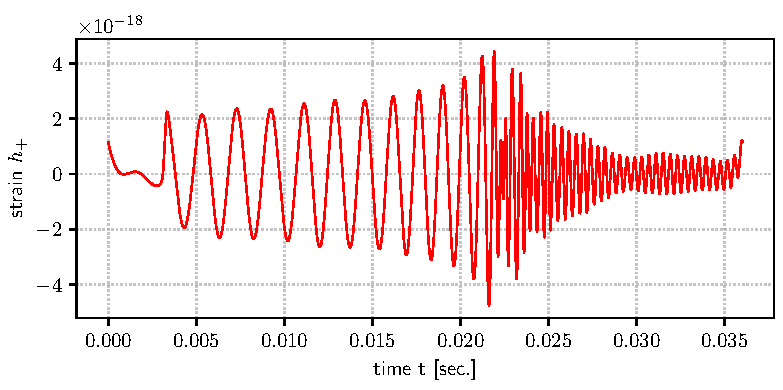
\includegraphics[width=.45\textwidth]{figures/Capitolo_3/SHT2.0.pdf}}\quad
	\subfloat[][\emph{SHT2.2}]
	{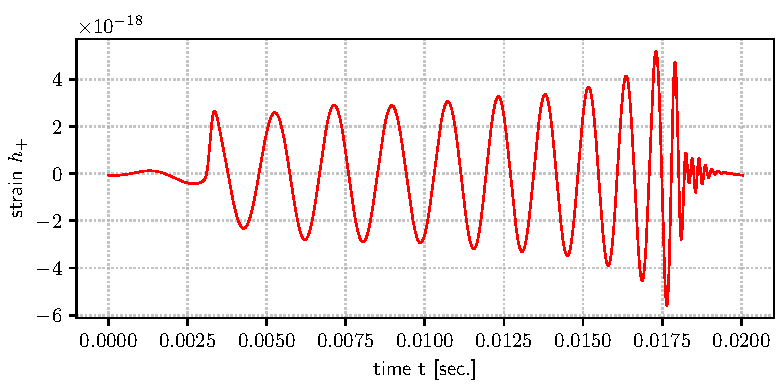
\includegraphics[width=.45\textwidth]{figures/Capitolo_3/SHT2.2.pdf}}
	\vspace{-5pt}
	\caption{Forme d'onda iniettate, per polarizzazione +, per l'equazione di stato SHT2, per le due configurazioni massive}
	\label{fig:forme_onda}
	\vspace{-15pt}
\end{figure}
\section{Ricostruzione di un evento simulato}
\label{subsection:APR4}
\begin{wraptable}{r}{0.4\textwidth}
	\vspace{-8pt}
	\begin{tabular}{cccccc}
		\toprule
		SNR	&$\rho$	&$c_{net}$	&ED	&$\theta$	&$\phi$	\\
		\midrule
		89.3	&36.8	&0.88	&-0.04	&321.7	&78.0	\\
		\bottomrule
	\end{tabular}
	\caption{Principali parametri dell'evento}
	\label{tab:parametri}
	\vspace{-10pt}
\end{wraptable}
Si riporta ora la ricostruzione di un singolo evento simulato a distanza $5$Mpc, con SNR sbiancato iniettato di 89.7 e posizione celeste $(\theta,\phi)=(321.6, 76.4)$deg.
Si riportano i principali coefficienti per identificare l'evento in figura \ref{tab:parametri}: il rapporto segnale su rumore (SNR); il valore del coefficiente $\rho$, ovvero una ranking statistic che esprime la significanza del segnale descrivendo l'energia coerente effettiva; il coefficiente $c_{net}$ descritto in equazione \ref{eqn:coefficient_energy}; ED che descrive lo sbilanciamento dell'energia tra i rivelatori nella rete e, infine, $\theta$ e $\phi$ che descrivono la posizione ricostruita della sorgente.
\begin{figure}[hbt!]
	\vspace{-10pt}
	\centering
	\subfloat[][\emph{LIGO-Livingstone}]
	{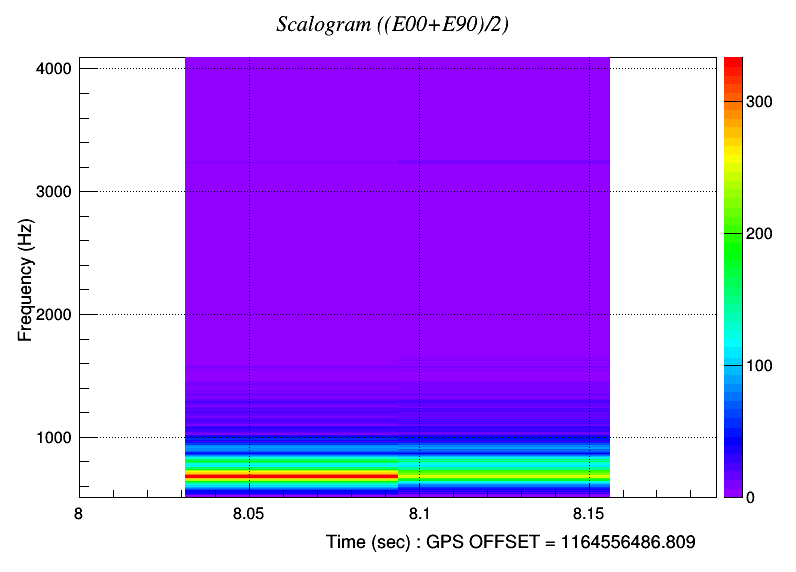
\includegraphics[width=.333333333\textwidth]{figures/Capitolo_3/APR4_q09/L1_wf_white_rec_tf.png}}
	\subfloat[][\emph{LIGO-Hanford}]
	{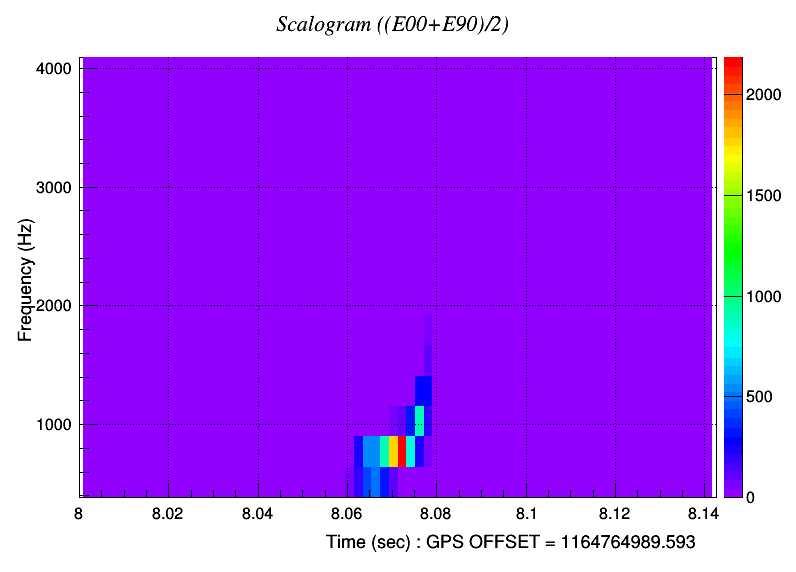
\includegraphics[width=.333333333\textwidth]{figures/Capitolo_3/APR4_q09/H1_wf_white_rec_tf.png}}
	\subfloat[][\emph{Virgo}]
	{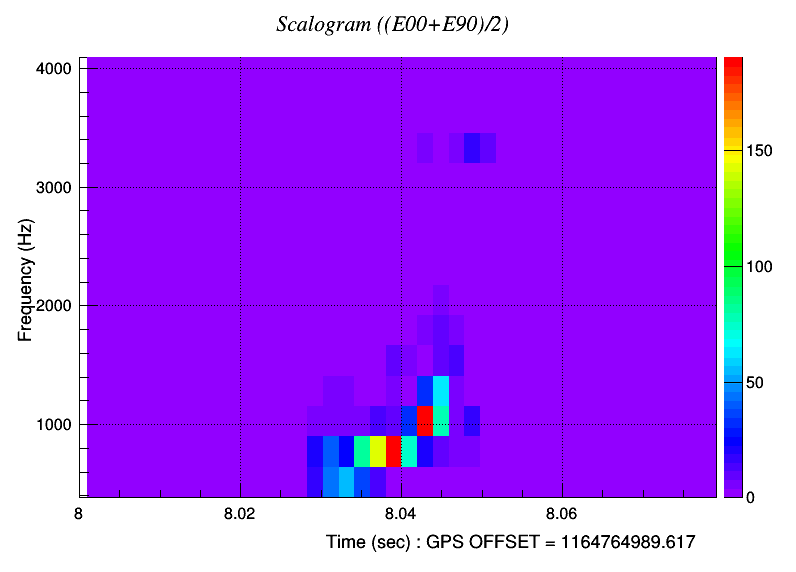
\includegraphics[width=.333333333\textwidth]{figures/Capitolo_3/APR4_q09/V1_wf_white_rec_tf.png}}
	\vspace{-8pt}
	\caption{Scalogrammi per ciascun rivelatore, che mostrano una rappresentazione sul piano tempo-frequenza del trigger}
	\label{fig:spettrogramma_apr4}
	\vspace{-10pt}
\end{figure}
Il segnale risulta immediatamente visibile negli scalogrammi dei tre rivelatori, nonostante la rivelazione di LIGO-Hanford risulti meno significativa. È interessante notare la differenza nell'istante di tempo della rivelazione, dovuta alla velocità finita dell'onda gravitazionale.

\begin{wrapfigure}{r}{0.4\textwidth}
	\vspace{-20pt}
	\begin{center}
		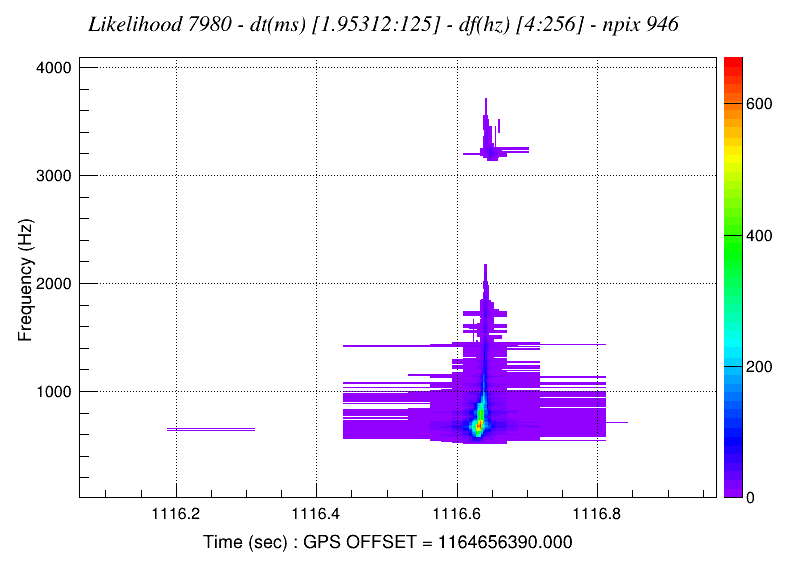
\includegraphics[width=0.4\textwidth]{figures/Capitolo_3/APR4_q09/l_tfmap_scalogram.png}
	\end{center}
	\vspace{-10pt}
	\caption{Mappa di verosimiglianza nel piano tempo-frequenza}
	\label{fig:Likelihood_APR4}
	\vspace{-10pt}
\end{wrapfigure}
Nel grafico della likelihood in Figura \ref{fig:Likelihood_APR4}, che descrive il contributo dell'energia totale del campione associato all'evento ricostruito, si osserva la parte conclusiva del tipico andamento a chirp, in cui la parte inferiore rappresenta lo spiraleggiamento fino alla coalescenza inclusa, mentre il cluster di dati in alto, a frequenze particolarmente elevate ($\smallsim 3.3$KHz) corrisponde all'emissione della post-coalescenza.
Infine nei grafici che seguono in Figura \ref{fig:strain_apr4} si osservano le ricostruzioni della forma d'onda, in particolare in nero è plottato il segnale iniettato nella simulazione, mentre in rosso il segnale ricostruito. Osservando il grafico delle frequenze si può notare come non sia stato ricostruito tra $\smallsim$2.5KHz e $\smallsim3$KHz, giustificando la separazione tra i cluster nel grafico della likelihood.
\begin{figure}[H]
	\vspace{-10pt}
	\centering
	\subfloat[][\emph{Dominio dei tempi}]
	{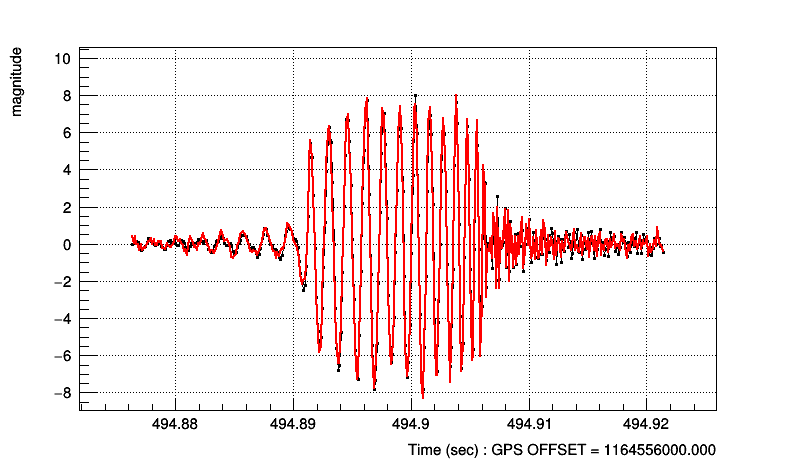
\includegraphics[width=.4\textwidth]{figures/Capitolo_3/APR4_q09/L1_wf_white_inj_rec.png}} \quad\quad
	\subfloat[][\emph{Dominio delle frequenze}]
	{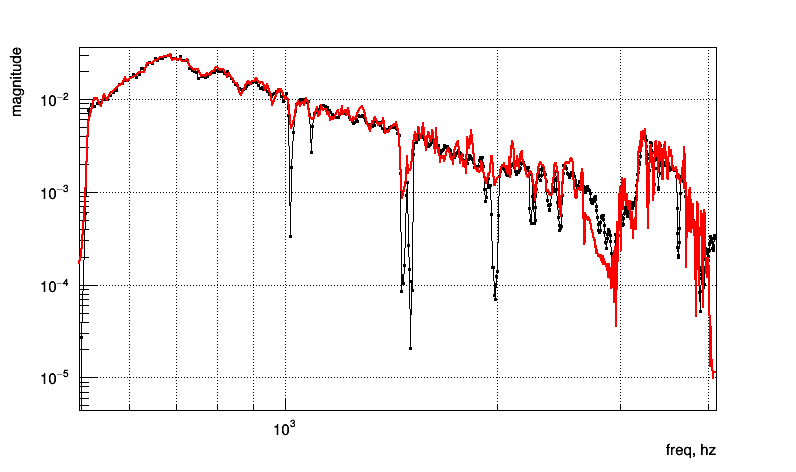
\includegraphics[width=.4\textwidth]{figures/Capitolo_3/APR4_q09/L1_wf_white_inj_rec_fft.png}}
	\vspace{-5pt}
	\caption{Ampiezza di strain ricostruita nel dominio dei tempi e nel dominio delle frequenze relative a un solo rivelatore}
	\label{fig:strain_apr4}
	\vspace{-15pt}
\end{figure}
%\paragraph{Equazione di stato SHT2}
%\label{subsection:SHT2}
Per le due forme d'onda con EOS SHT2 si presentano solo i grafici delle likelihood, entrambi gli eventi hanno un SNR iniettato sbiancato di $\smallsim 65$, e sono simulati ad una distanza di $2.5$Mpc. le due forme d'onda iniettate differiscono per la massa delle NS per la coalescenza, in particolare nella Figura \ref{fig:likelihood_sht2}(a), con masse tali da andare in ipermassiva, si può notare come sia presente un segnale di post-merger a $\smallsim 2.5$kHz mentre nella Figura \ref{fig:likelihood_sht2}(b) che riporta la simulazione di un evento con decadimento diretto in un buco nero, non vi è nessun segnale di post-coalescenza ma solo un segnale di spiraleggiamento e coalescenza che arriva ad alte frequenze. 
\begin{figure}[H]
	\vspace{-20pt}
	\centering
	\subfloat[][\emph{SHT2.0}]
	{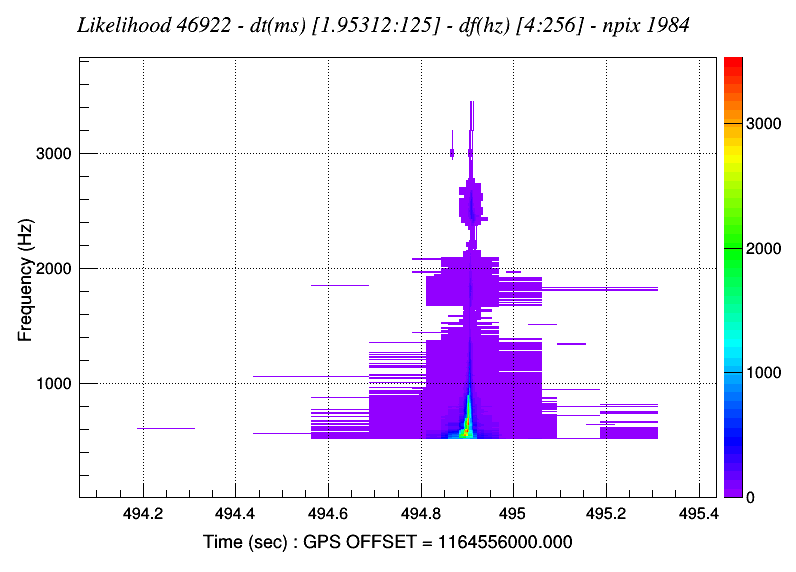
\includegraphics[width=.5\textwidth]{figures/Capitolo_3/SHT2.0spinf1_1/l_tfmap_scalogram.png}}
	\subfloat[][\emph{SHT2.2}]
	{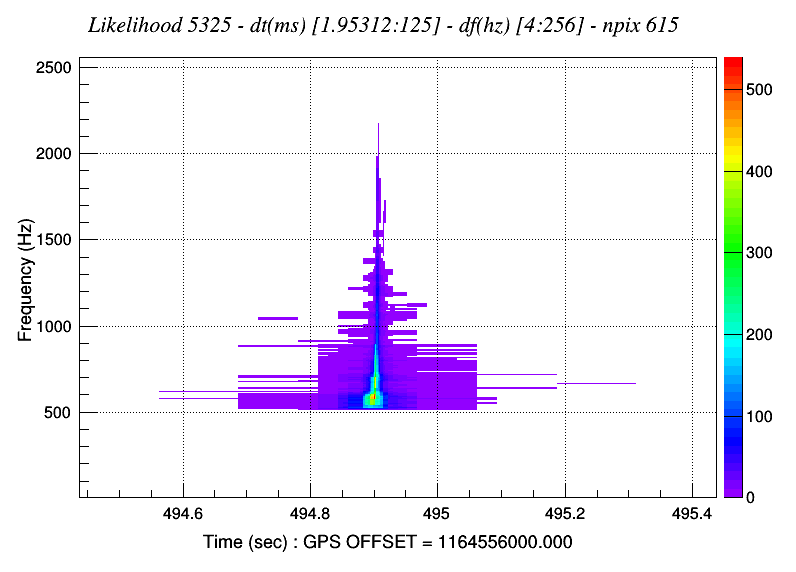
\includegraphics[width=.5\textwidth]{figures/Capitolo_3/SHT2.2spinf1_1/l_tfmap_scalogram.png}}
	\vspace{-5pt}
	\caption{Mappe di verosimiglianza ricostruite per le due forme d'onda iniettate}
	\label{fig:likelihood_sht2}
	\vspace{-15pt}
\end{figure}

\section{Caratteristiche degli eventi simulati}
\label{subsection:cwb_injections}
%La post coalescenza, come già detto, è allo stato attuale difficile da rivelare a causa della scarsa sensibilità dei rivelatori a tali frequenze, per questo le analisi che vengono fatte in questa tesi non coivolgeranno dati misurati, ma dati simulati che vengono iniettati in rumore gaussiano, anch'esso simulato.\\
È stato simulato un considerevole numero di eventi ($\smallsim 5000$ eventi per forma d'onda), che vengono poi analizzati con l'algoritmo cWB per verificarne la capacità di ricostruzione e studiare questi eventi.\\
Gli eventi simulati vengono prodotti a 5 diverse distanze [20, 10, 5, 2.5, 1.25]Mpc e con posizione della sorgente distribuita in modo uniforme nel cielo (Figura \ref{fig:skypos}(b)), con polarizzazione del segnale simulata anch'essa con distribuzione uniforme.
\begin{figure}[hbt!]
	\vspace{-20pt}
	\centering
	\subfloat[][\emph{Distribuzione distanze}]
	{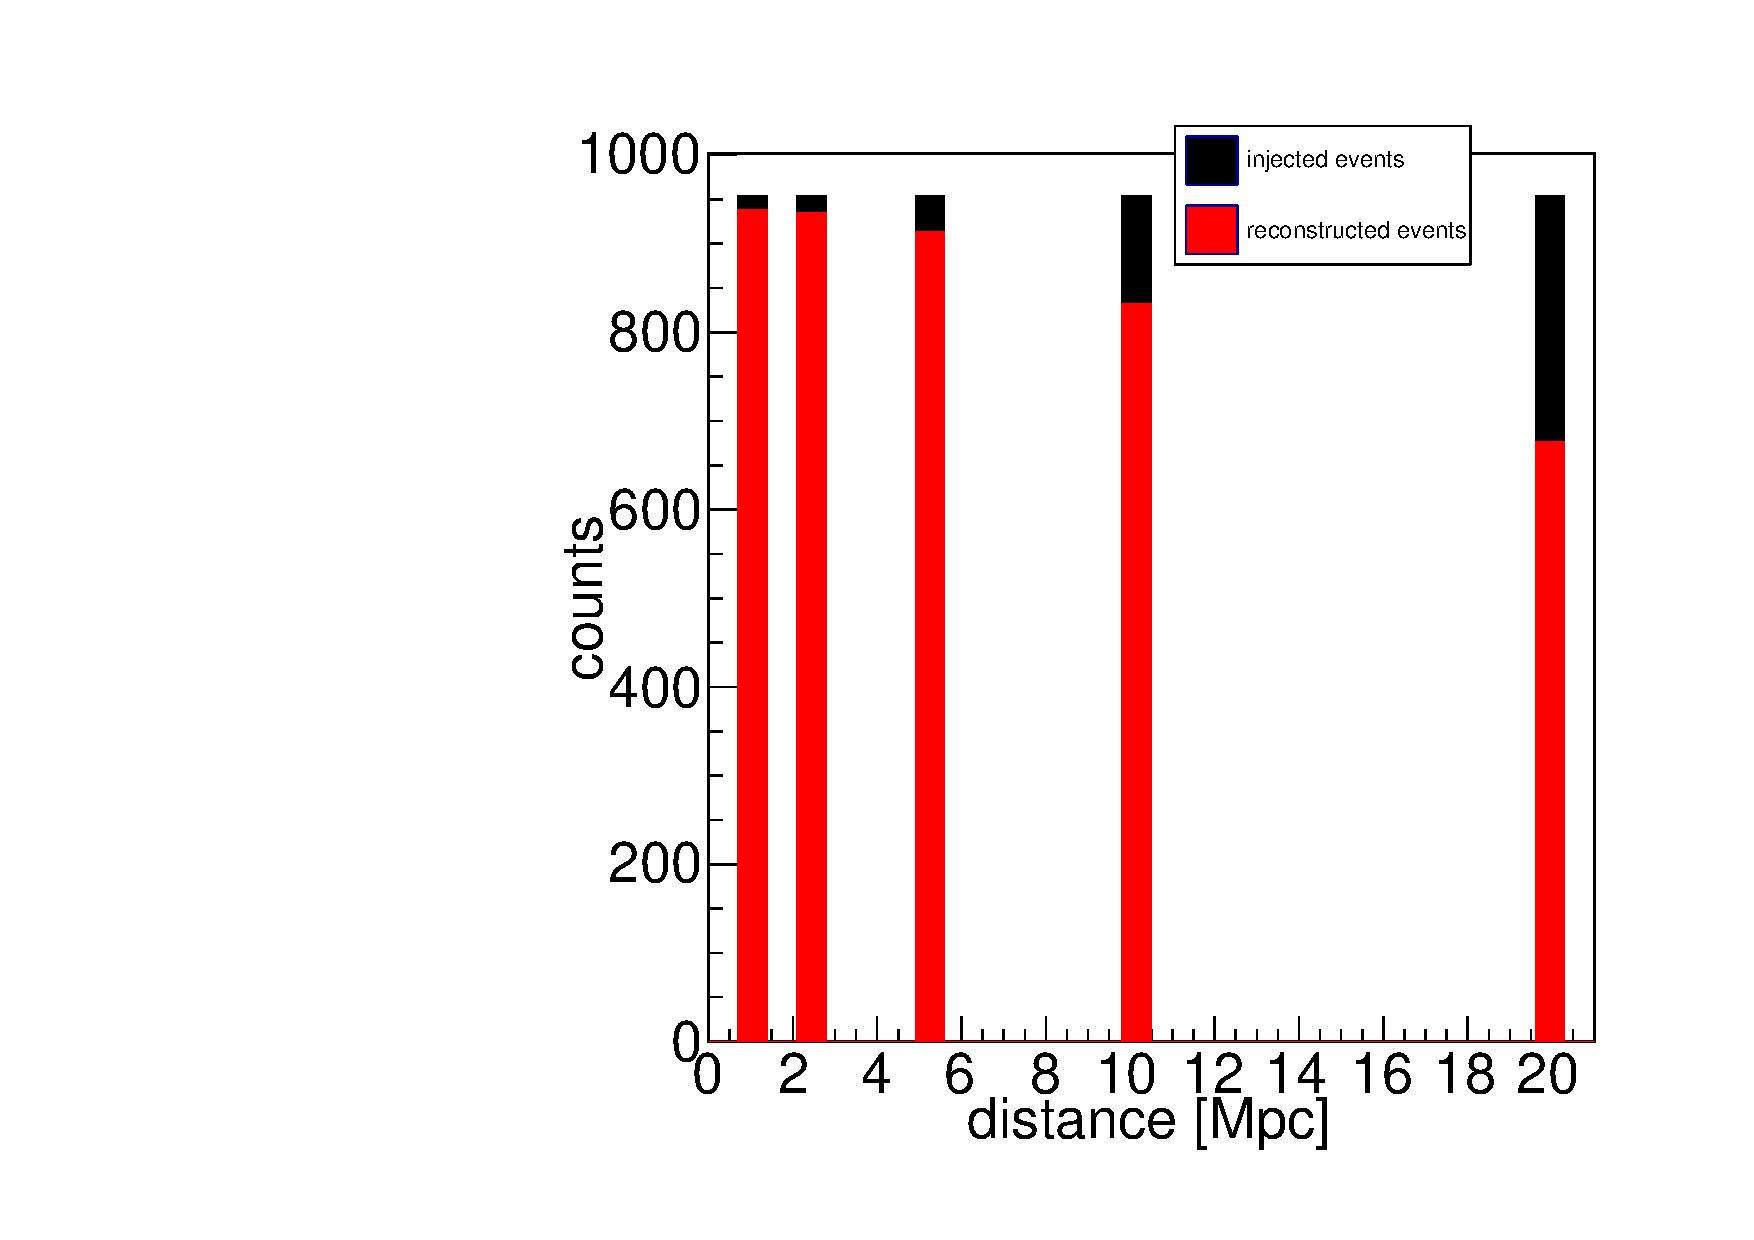
\includegraphics[width=.3\textwidth]{figures/Capitolo_3/report/RfactorsSHT2_0spin1.pdf}}\quad
	\subfloat[][\emph{Distribuzione celeste}]
	{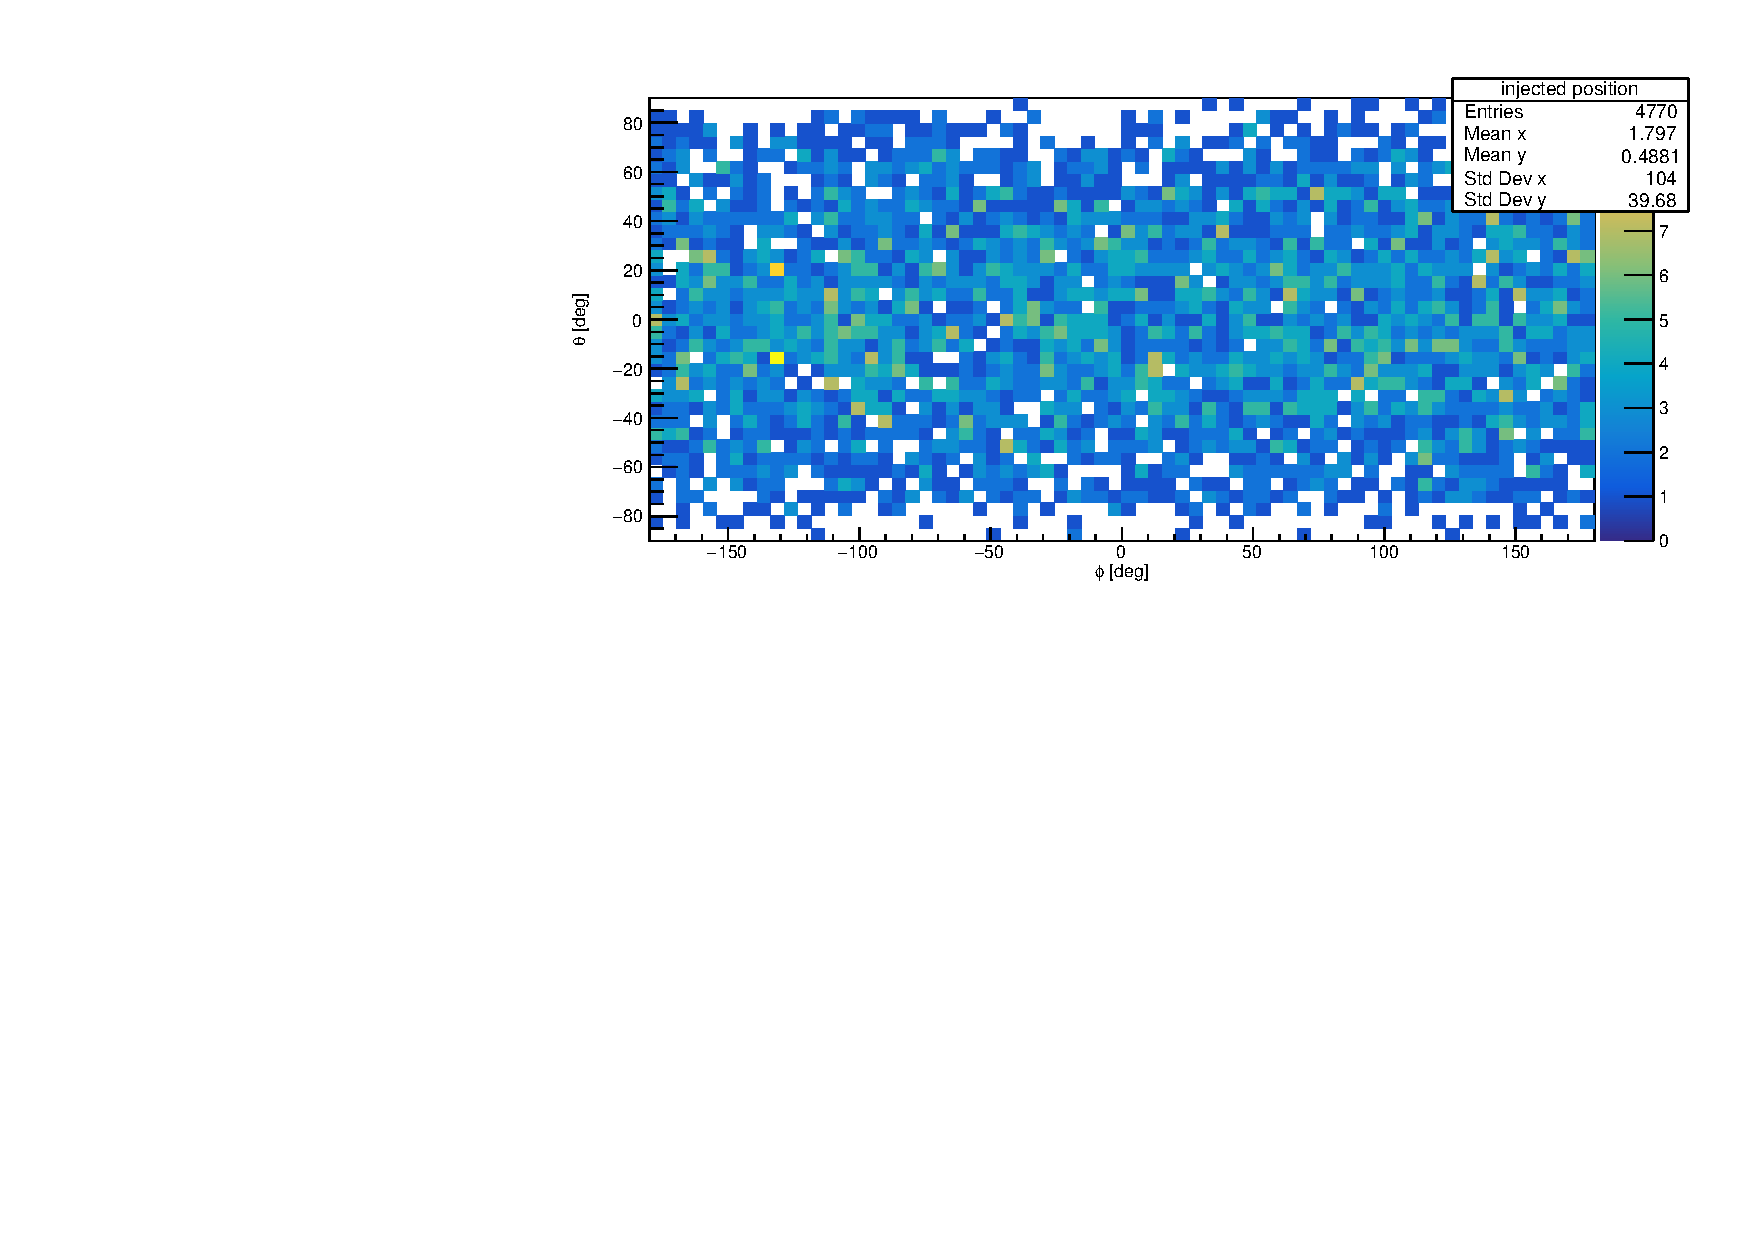
\includegraphics[width=.6\textwidth]{figures/Capitolo_3/report/ipositionSHT2_0spin1.pdf}}
	\vspace{-5pt}
	\caption{Distribuzione degli eventi simulati per l'EOS SHT2.0}
	\label{fig:skypos}
	\vspace{-10pt}
\end{figure}
Si riporta poi, in Figura \ref{fig:SNR_INJ_REC_COUNTS}, la distribuzione degli SNR, in funzione della distanza di iniezione. Si nota immediatamente come al crescere della distanza il rapporto segnale su rumore iniettato decresce, mentre per gli eventi molto vicini gli SNR arrivino a grandezze considerevoli. \\
\begin{figure}[hbt!]
	\vspace{-30pt}
	\centering
	\subfloat[][\emph{SHT2.0}]
	{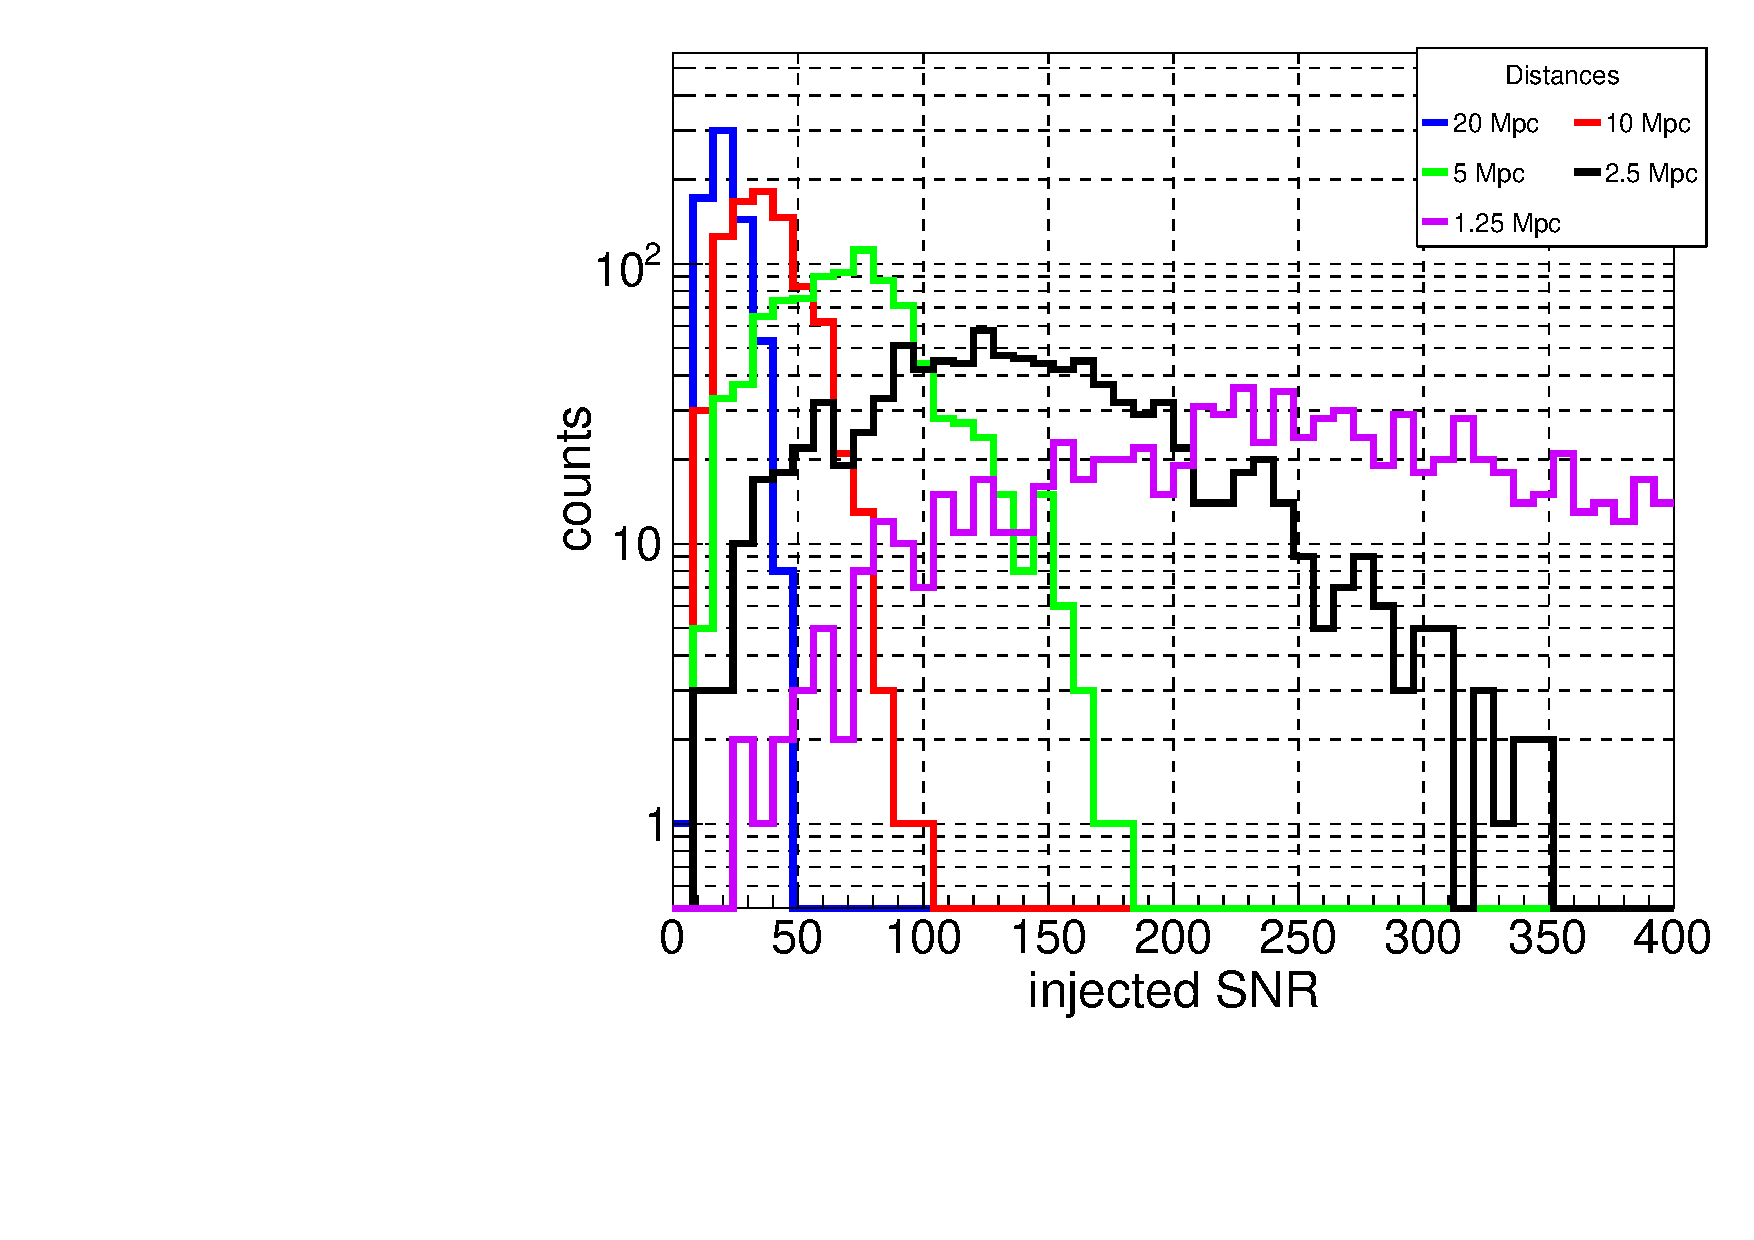
\includegraphics[width=.333333333333333333\textwidth]{figures/Capitolo_3/report/Network_iSNR_FactorsSHT2_0spin1.pdf}}
	\subfloat[][\emph{SHT2.2}]
	{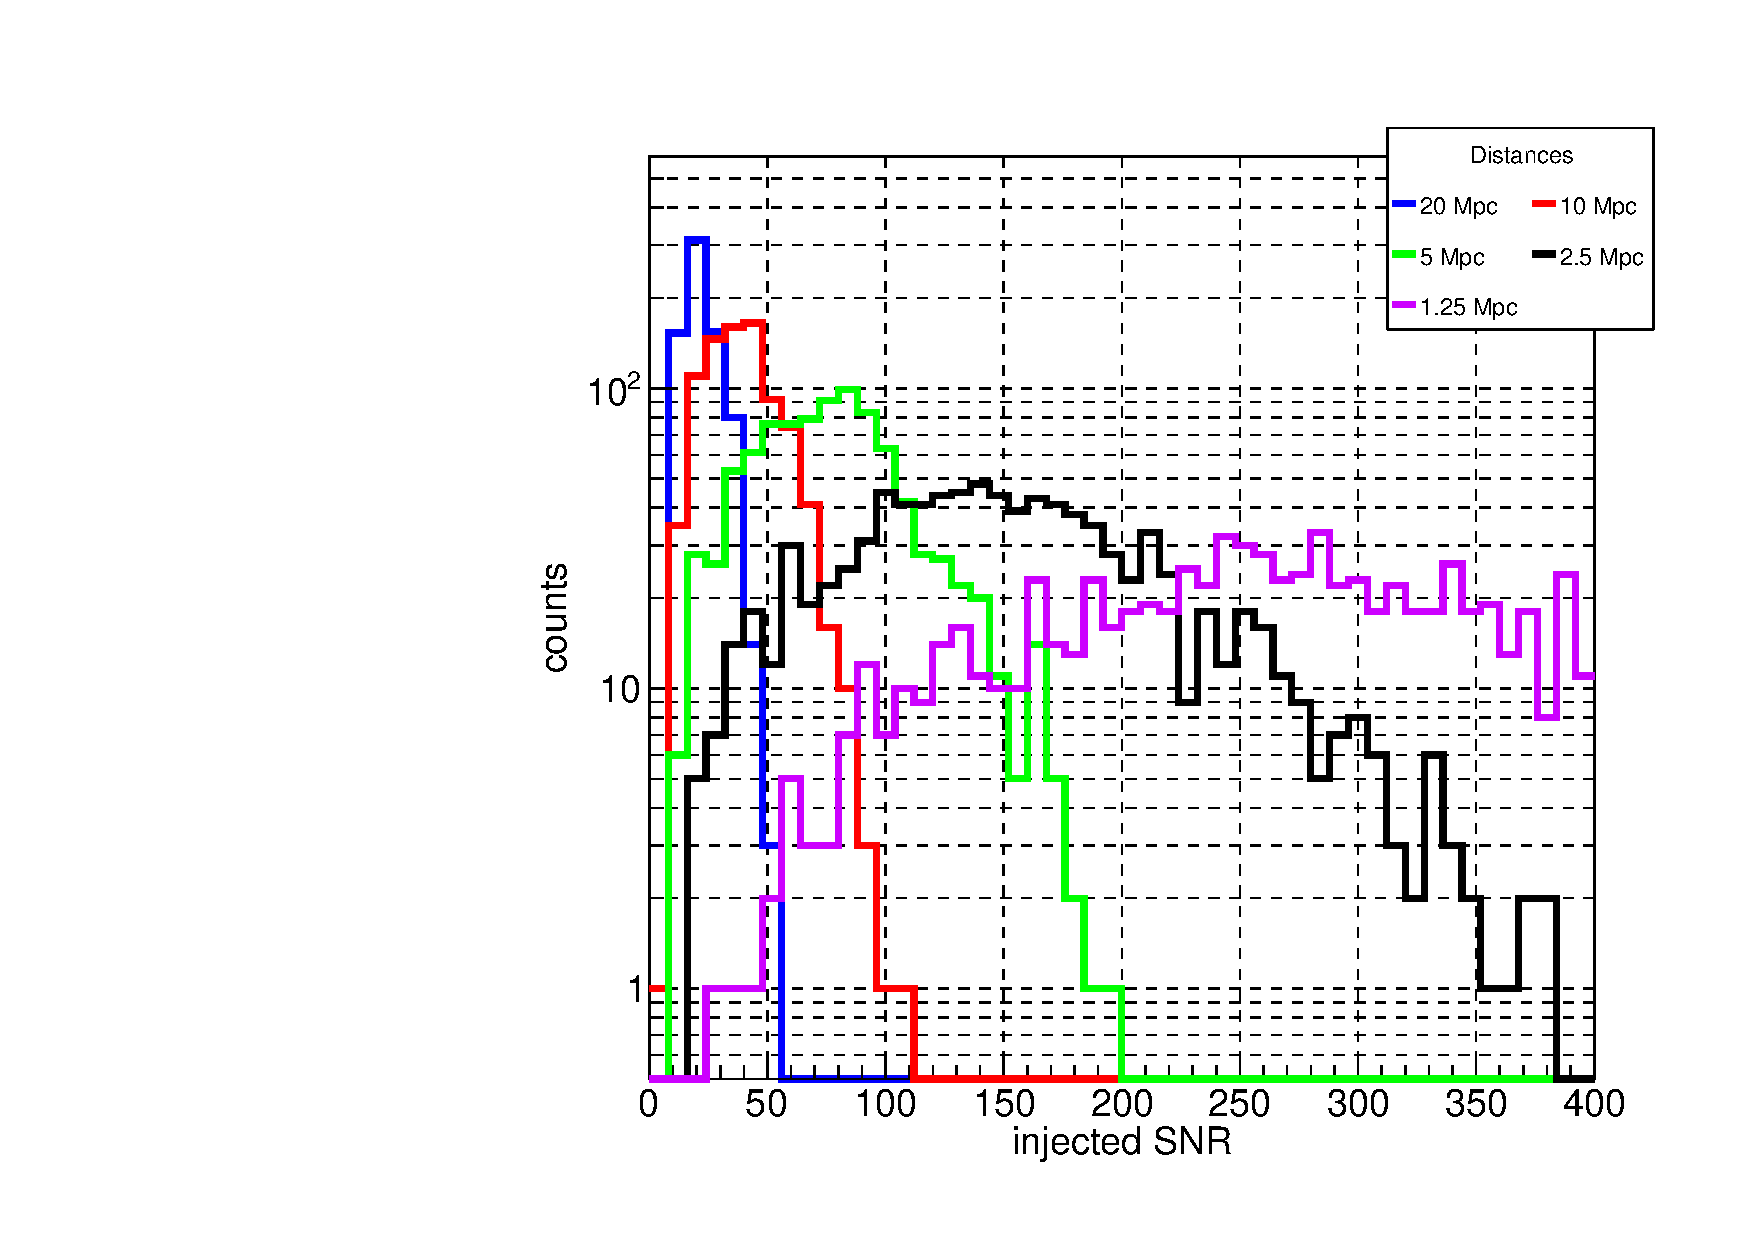
\includegraphics[width=.333333333333333333\textwidth]{figures/Capitolo_3/report/Network_iSNR_FactorsSHT2_2spin1.pdf}}
	\subfloat[][\emph{APR4}]
	{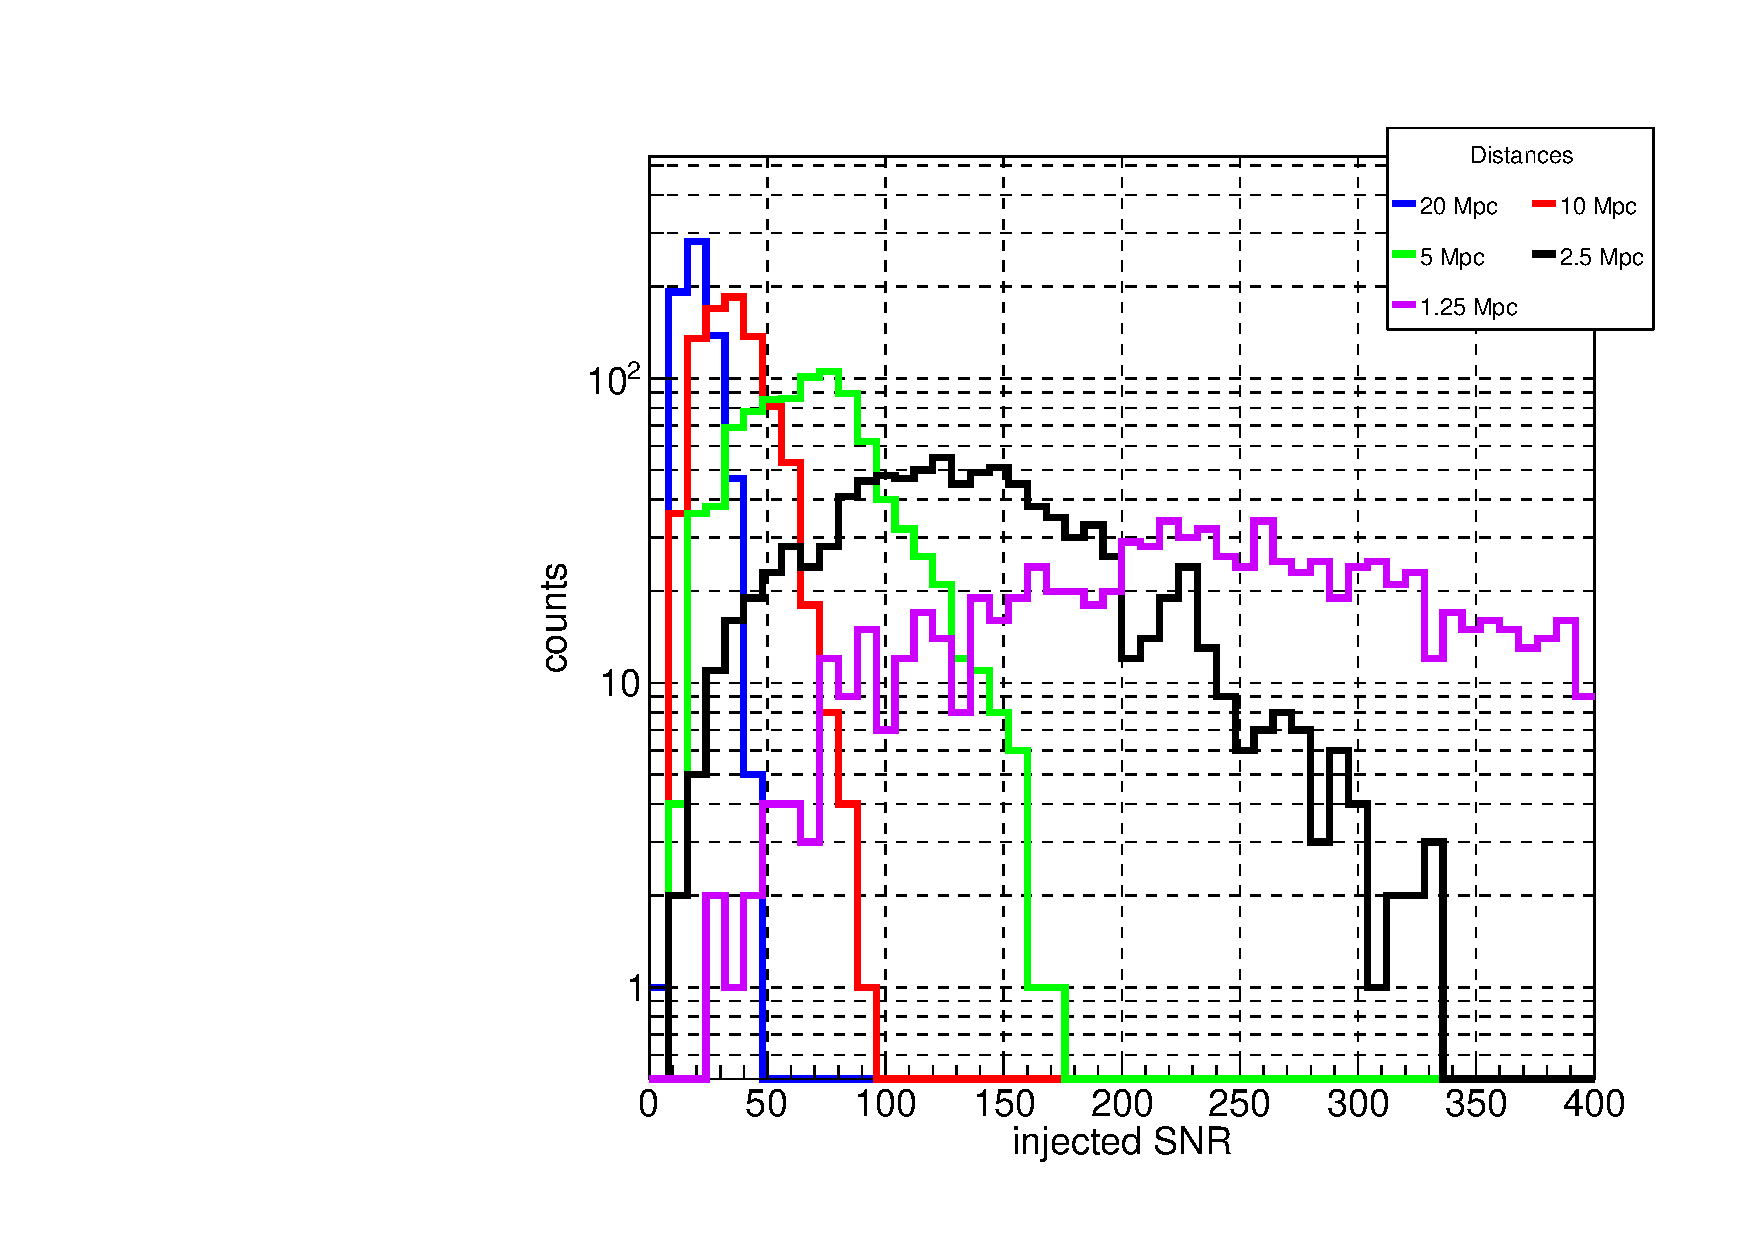
\includegraphics[width=.333333333333333333\textwidth]{figures/Capitolo_3/report/Network_iSNR_FactorsAPR4_q09.pdf}}
	\vspace{-8pt}
	\caption{SNR iniettato per le tre EOS, diviso nelle distanze}
	\label{fig:SNR_INJ_REC_COUNTS}
	\vspace{-15pt}
\end{figure}

\begin{wrapfigure}{r}{0.5\textwidth}
	\vspace{-15pt}
	\begin{center}
		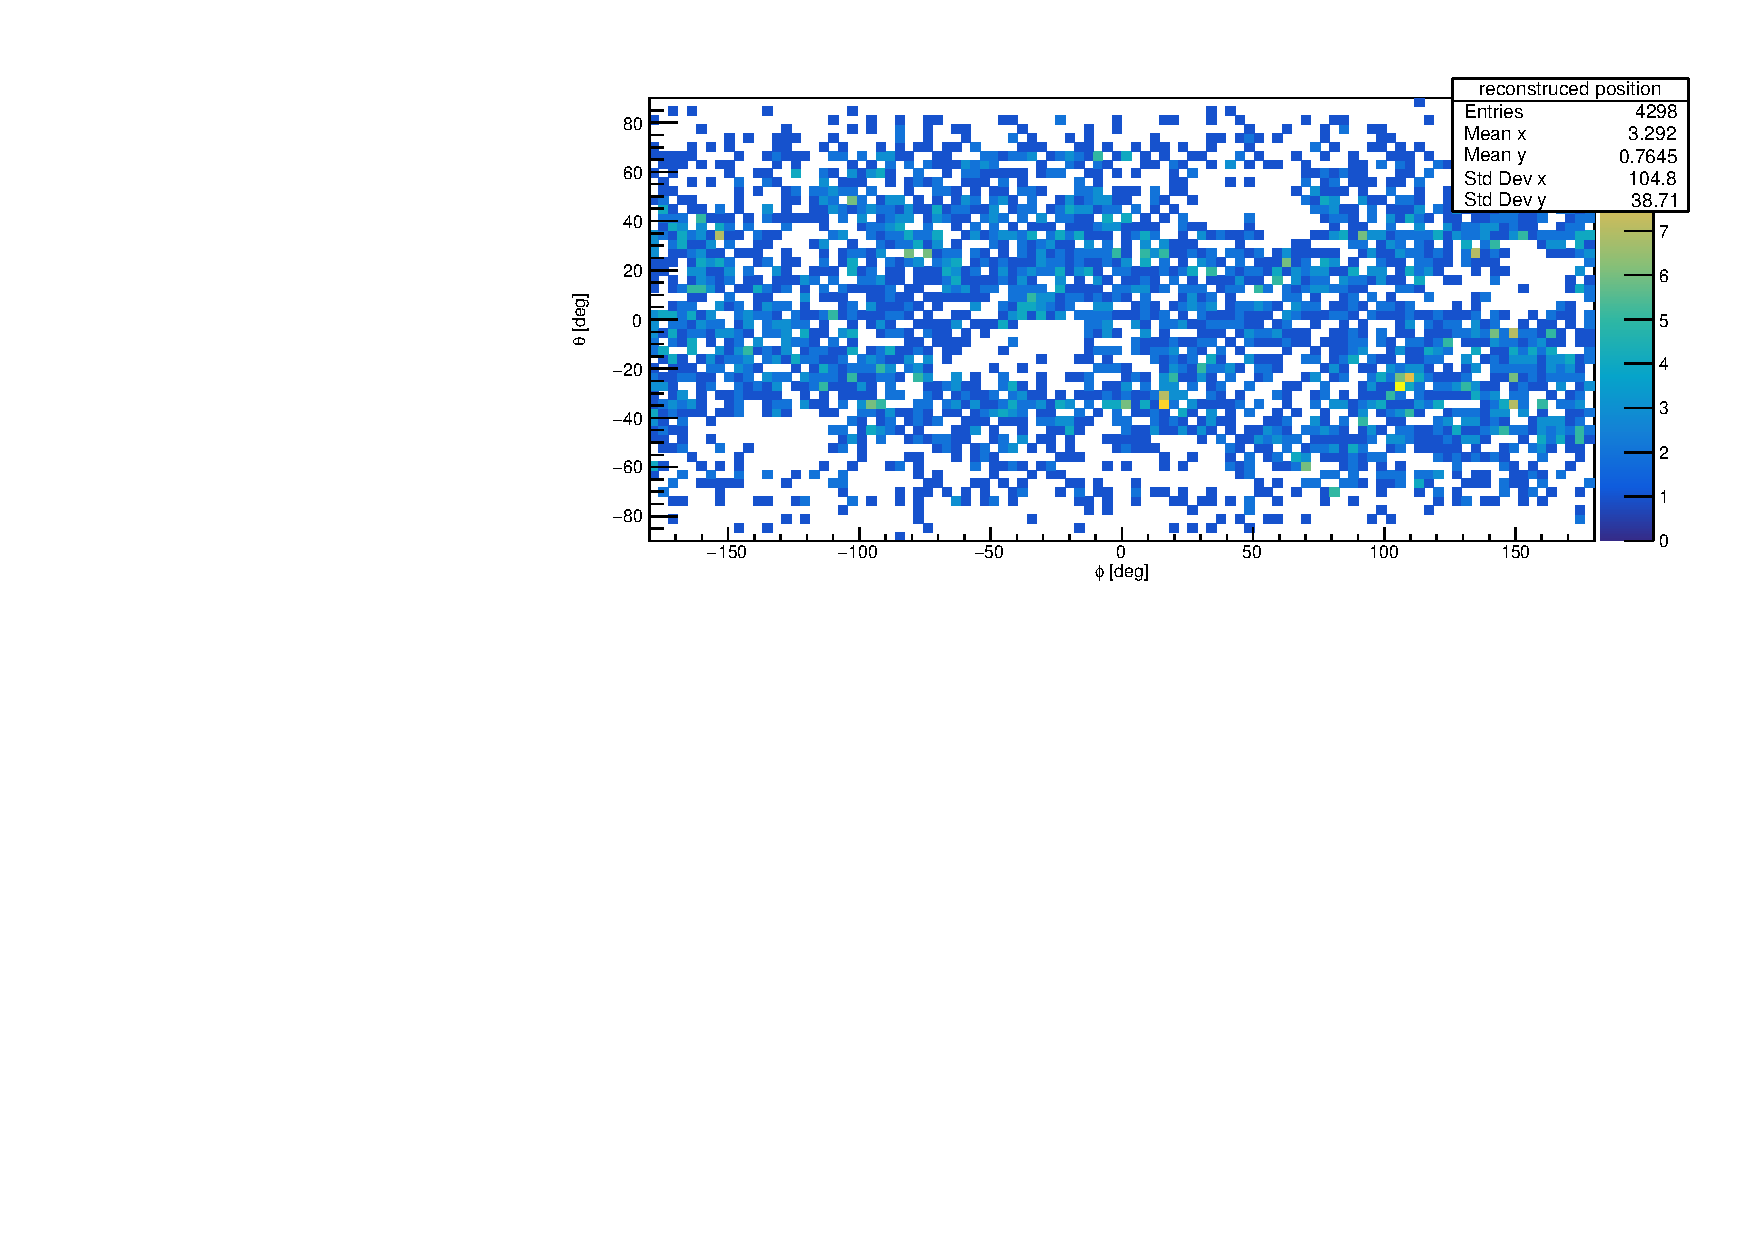
\includegraphics[width=0.5\textwidth]{figures/Capitolo_3/report/RopositionSHT2_0spin1.pdf}
	\end{center}
	\vspace{-10pt}
	\caption{Distribuzione degli eventi ricostruiti per l'EOS SHT2.0}
	\label{fig:skyposrec}
	\vspace{-15pt}
\end{wrapfigure}
Gli eventi che vengono ricostruiti, come si osserva in Figura \ref{fig:skypos}(a), non sono tutti quelli iniettati, ma solo la parte di essi (4298/4770) che viene rivelata con SNR sopra al valore di soglia nella rete. Si riportano in Figura \ref{fig:skyposrec} le distribuzioni degli eventi ricostruiti che sono da confrontare con Figura \ref{fig:skypos}(b), si nota che vi sono evidenti buchi, che giustificano ulteriormente la mancata ricostruzione: esistono punti ciechi della rete. L'aggiunta nei prossimi run di altri rivelatori risolverà almeno in parte questa problematica. 

\section{Curve di sensibilità e analisi dell'overlap}
\label{section:overlap}
Prima di riportare l'analisi si fa una precisazione: per gli eventi con equazione di stato APR4 è stato necessario effettuare ulteriore un passaggio: essendo per questa EOS il segnale di post-coalescenza a frequenze particolarmente elevate si genera un problema nella ricostruzione: i segnali di coalescenza e quelli di post-coalescenza venivano spezzati in due eventi separati. L'effetto descritto si può notare nei grafici in Figura \ref{fig:Overlap_problem}, dove si vede un inconsistenza nella curva di overlap (a sinistra) che viene spiegata dagli eventi spezzati: nel grafico delle frequenze massime e minime si vede infatti un gruppo di eventi che ha frequenza minima estremamente alta, comportamento incompatibile con l'andamento che assume un evento ricostruito in modo completo, che come descritto in precedenza dovrebbe avere l'andamento di un chirp, partendo da frequenza basse fino a un picco.\\
%Per ovviare a tale problematica la strategia adottata ha previsto inizialmente il tentativo di allargare la forbice delle frequenze aumentando il valore di soglia da 128Hz fino a 512Hz, con il rischio, però di andare a raccogliere eccessi di rumore e avendo come risultato un segnale non pulito. Il tentativo non ha tuttavia risolto il problema: nella maggioranza dei casi il segnale di coalescenza viene ricostruito a partire da una frequenza più distante di 512Hz rispetto alla fine del segnale di coalescenza, causando una stima peggiore del segnale complessivo senza un significativo miglioramento sul segnale di post-coalescenza. \\
Per ovviare a tale problema la procedura di caratterizzazione del segnale di post-coalescenza è stata applicata dopo aver selezionato per ogni evento simulato solamente la ricostruzione che comprendeva la fase di spiraleggiamento e coalescenza, in quanto parte più energetica, escludendo dall'analisi la parte meno energetica dell'evento ricostruto spezzato. Questo taglio viene poi applicato anche alle altre EOS considerate, poiché le caratterizzazioni fatte devono essere coerenti per BNS indipendentemente dal modello considerato.
%Il problema è invece stato risolto utilizzando un comando di cWB che permette, a partire dalle ricostruzioni, di tagliare, tra gli eventi spezzati, l'evento meno energetico. In questo modo si perde parte degli eventi ricostruiti ma vengono risolte le incongruenze.
\begin{figure}[hbt!]
	\vspace{-20pt}
	\centering
	\subfloat[][\emph{Overlap}]
	{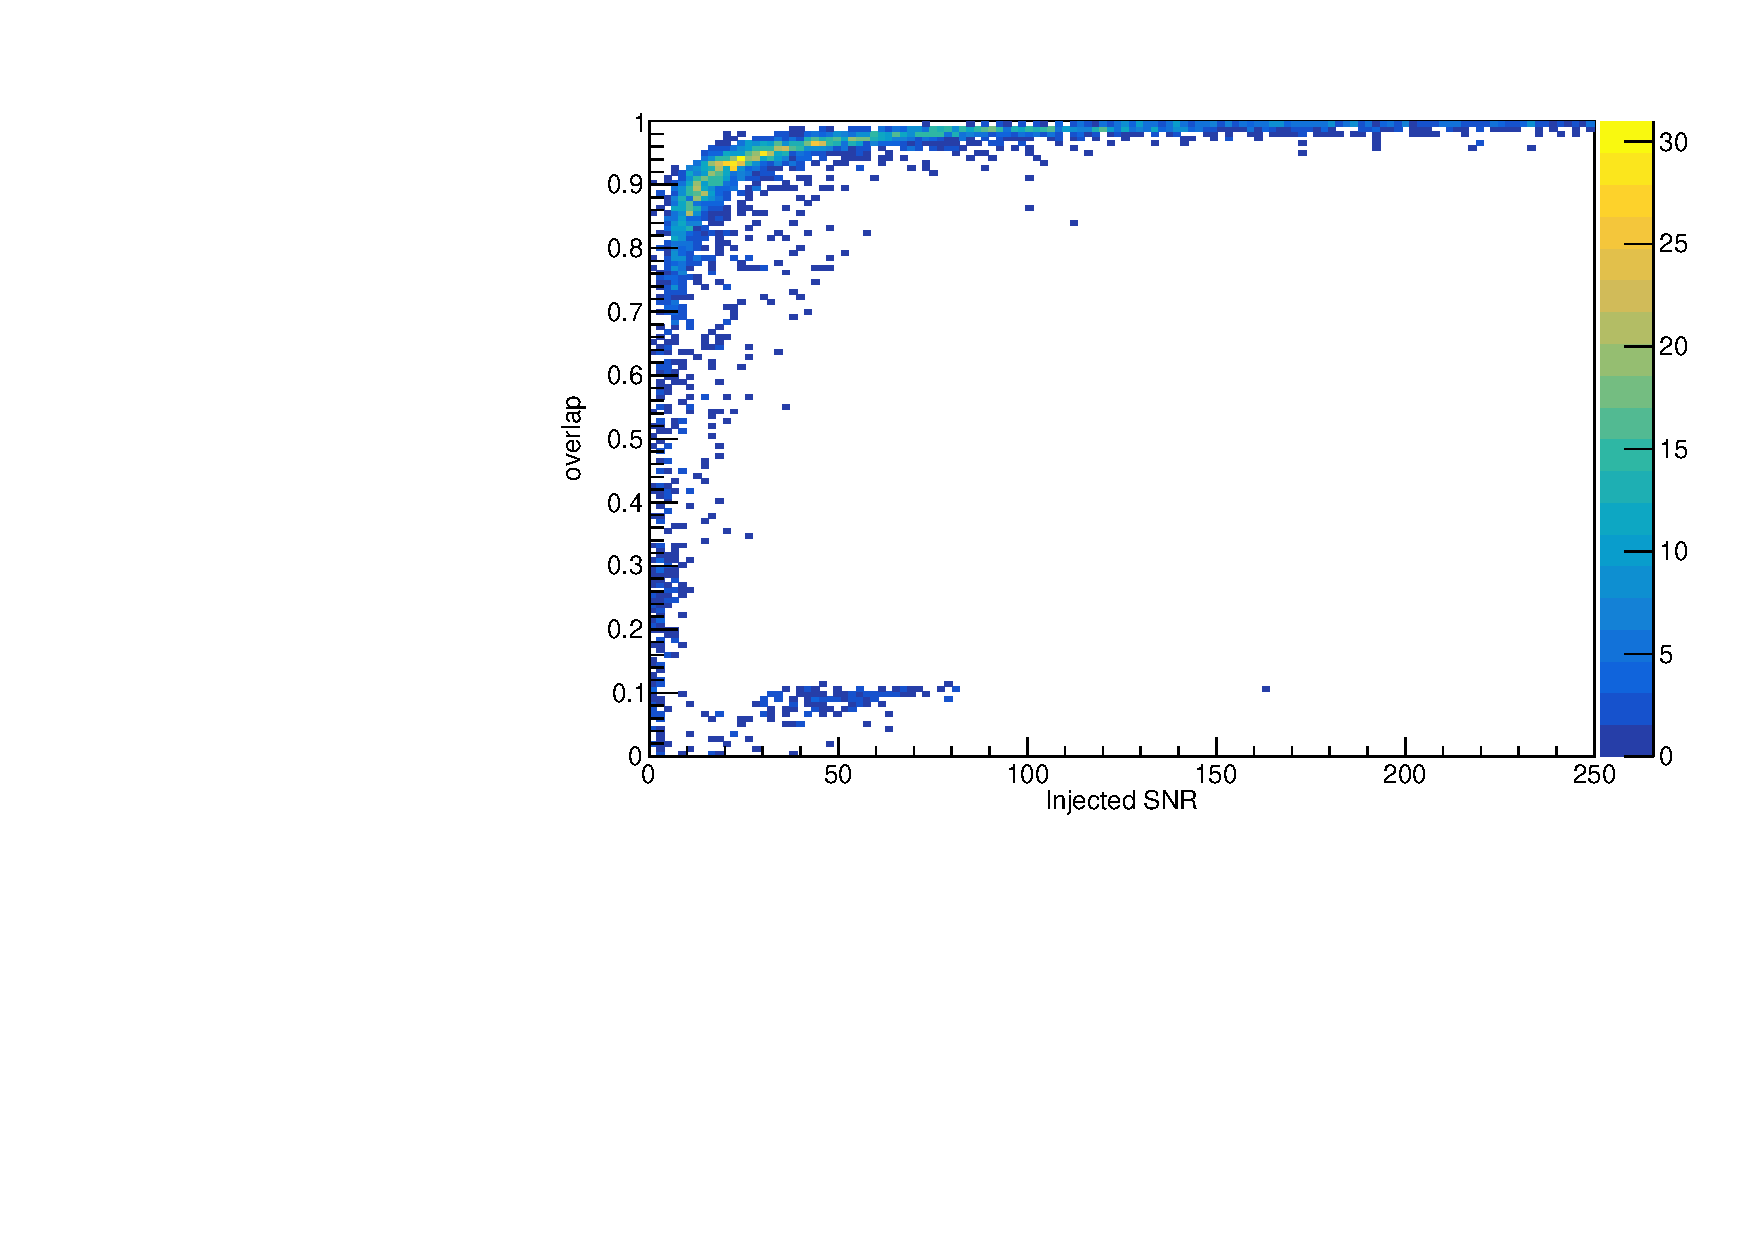
\includegraphics[width=.4\textwidth]{figures/Capitolo_3/OverlapDistributionDetector1APR4_q09.pdf}}
	\subfloat[][\emph{Frequenza minima e massima}]
	{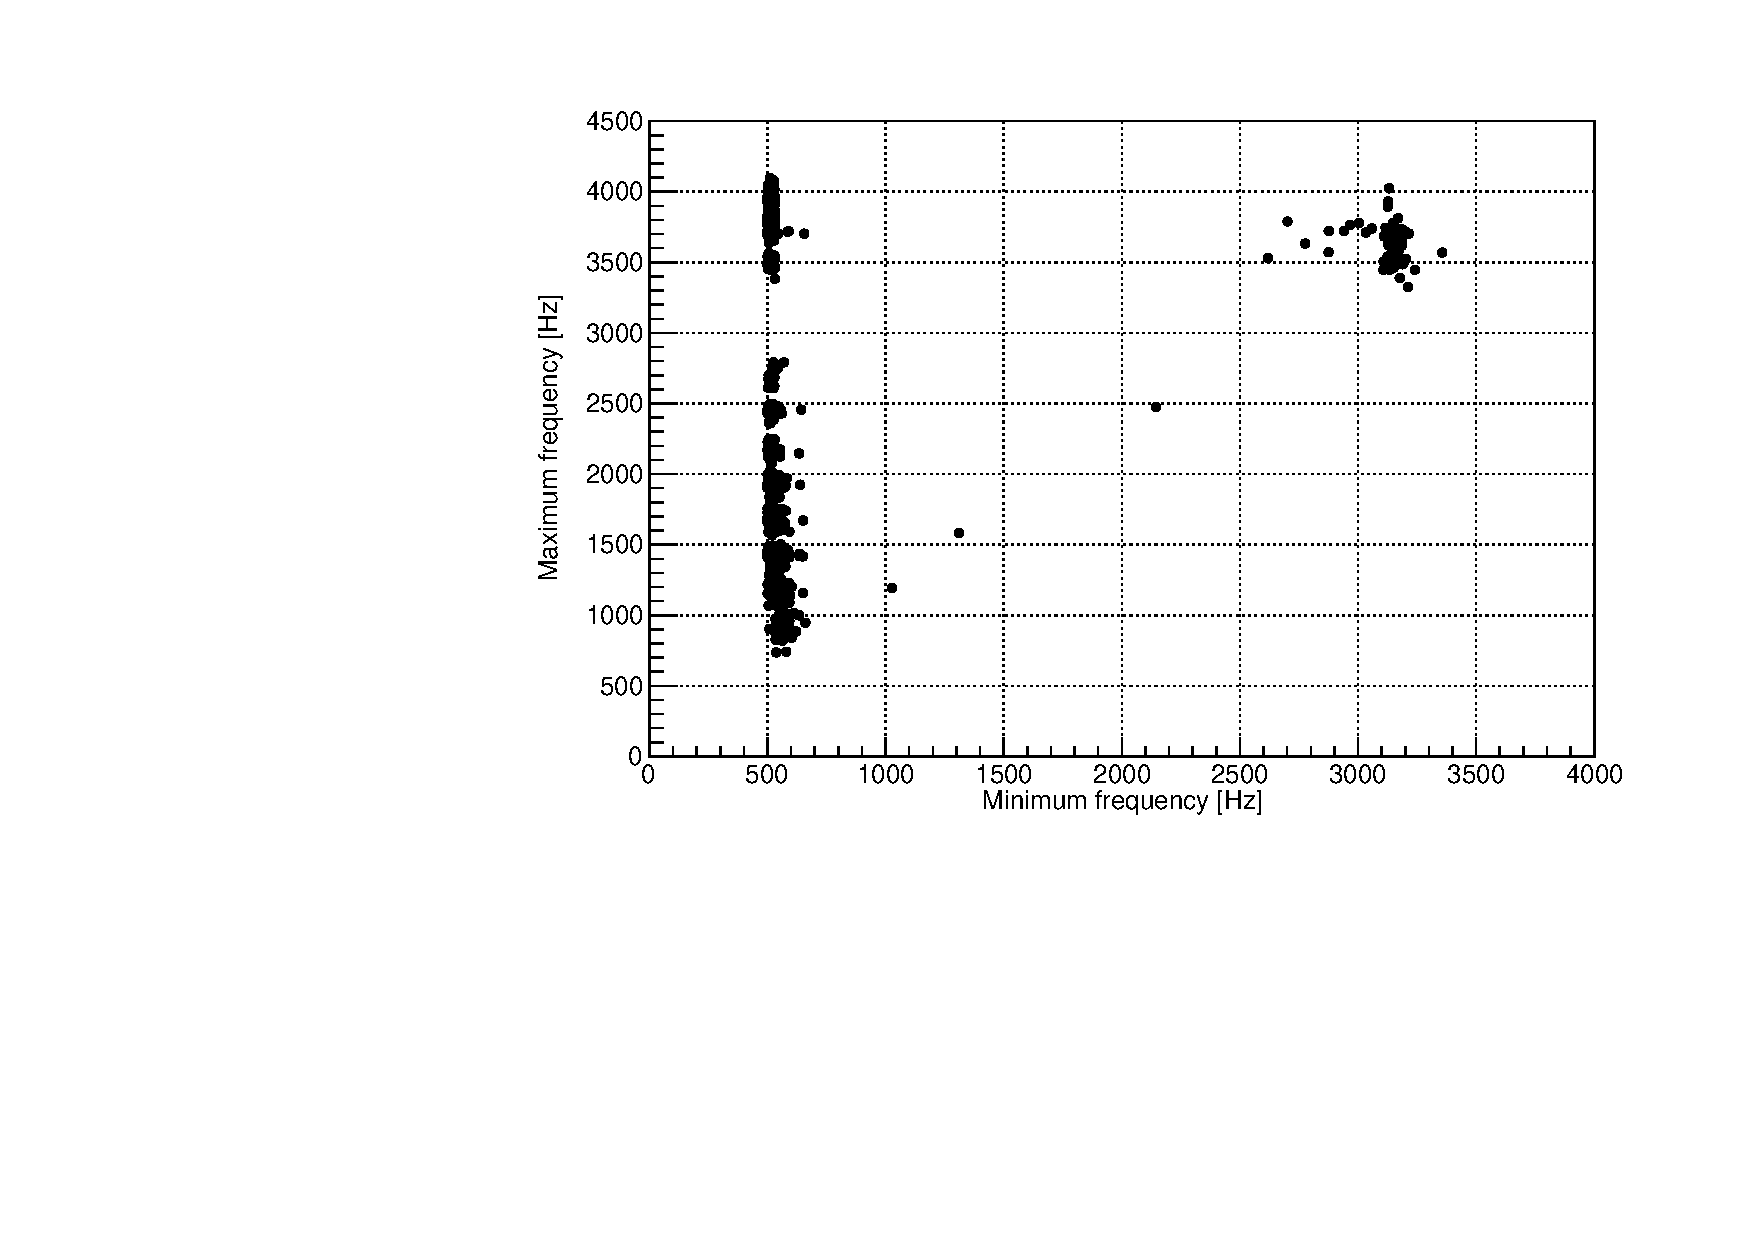
\includegraphics[width=.4\textwidth]{figures/Capitolo_3/FrequencyLHDistributionDetector1APR4_q09.pdf}}
	\vspace{-5pt}
	\caption{Distribuzione degli overlap e della frequenza massima ricostruita in funzione della minima}
	\label{fig:Overlap_problem}
	\vspace{-10pt}
\end{figure}

Si procede quindi a verificare in modo quantitativo l'efficienza dell'algoritmo di ricostruizione, facendo un fit degli SNR ricostruiti in funzione degli SNR iniettati, il cui grafico per la EOS SHT2.0 è in Figura \ref{fig:overlap}, mentre per le altre EOS i risultati sono analoghi. L'andamento ideale che ci si aspetta è rappresentato dalla bisettrice del primo e terzo quadrante, che corrisponde a una processo tale per cui l'SNR ricostruito è pari a quello iniettato.
\begin{figure}[hbt!]
	\vspace{-5pt}
	\centering
	{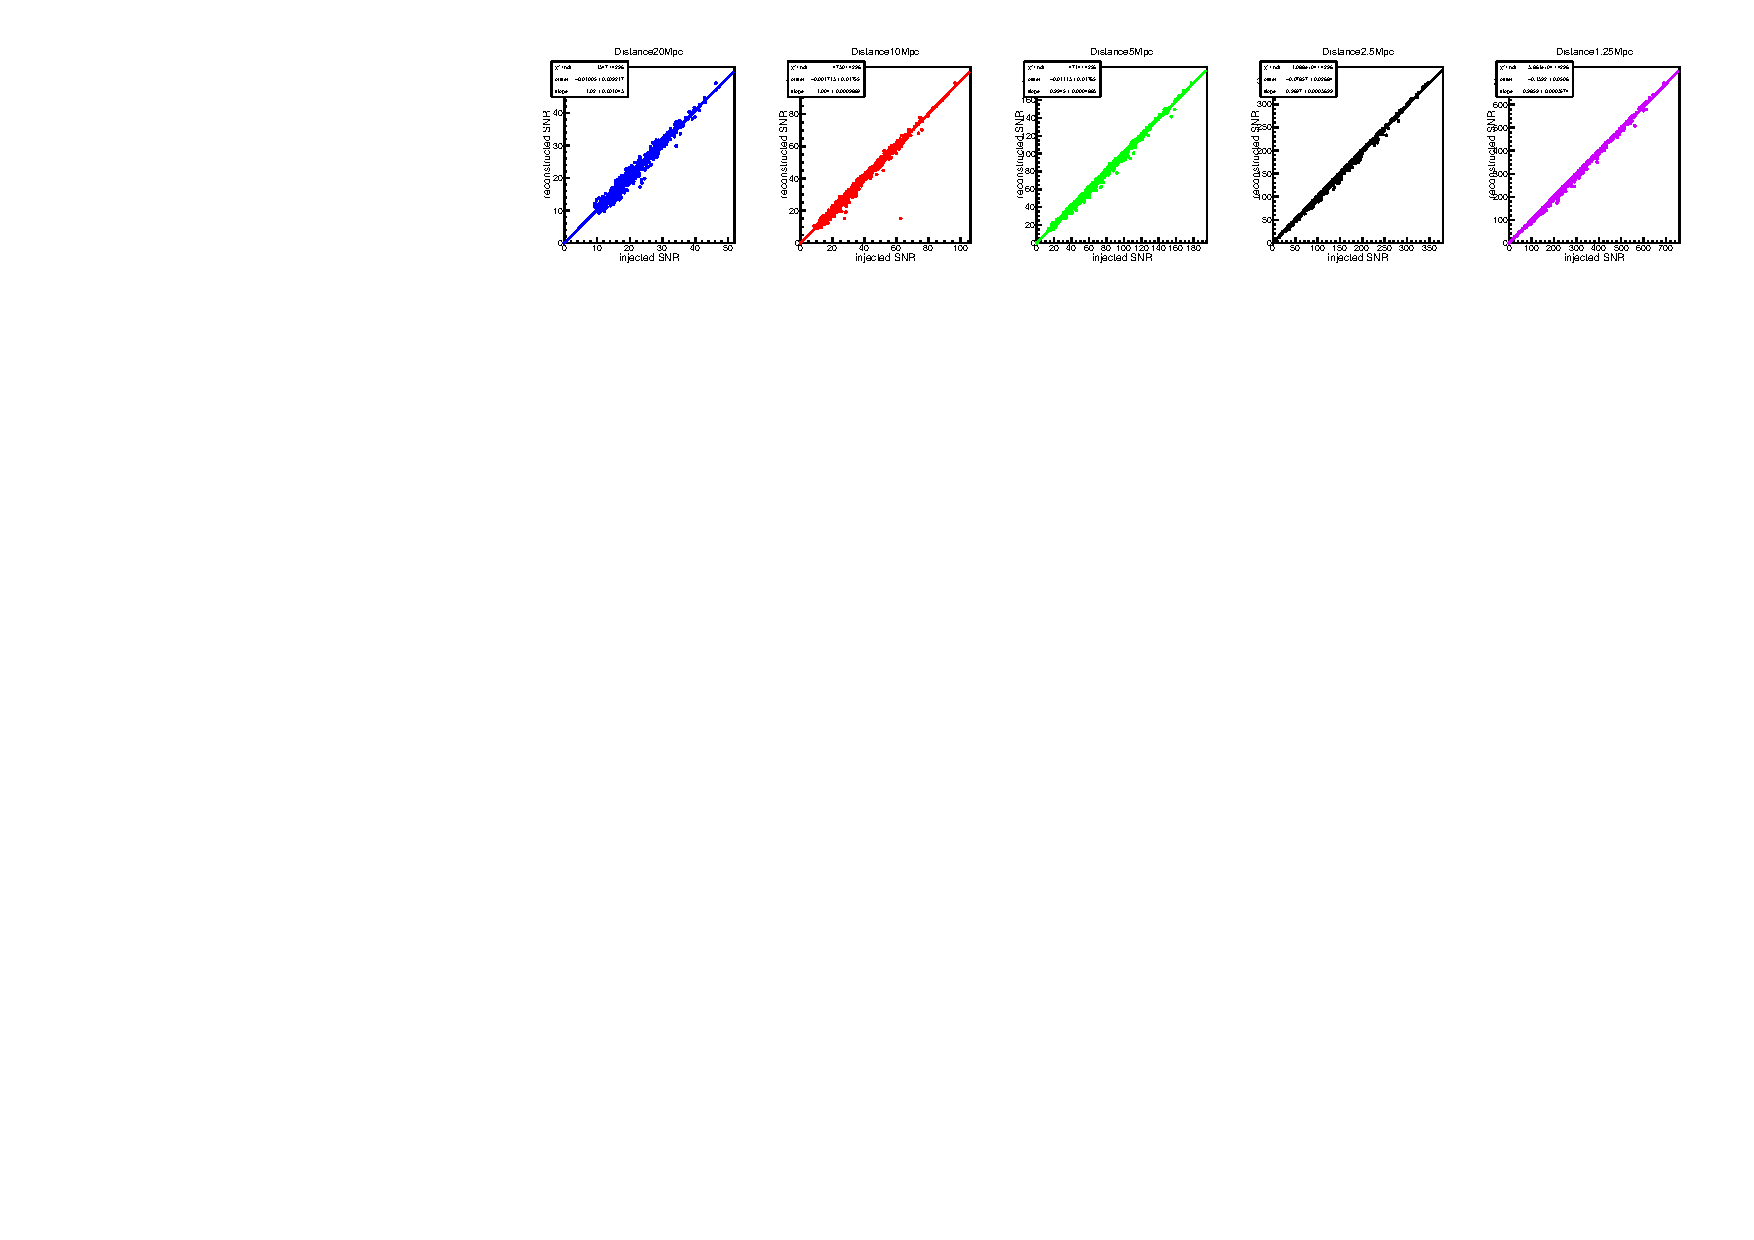
\includegraphics[width=1\textwidth]{figures/Capitolo_3/report/FITSHT2_0spin1.pdf}}
	\vspace{-15pt}
	\caption{Grafico dell'SNR ricostruito in funzione dell'iniettato per la EOS SHT2.0 divisi per distanze di iniezione}
	\label{fig:overlap}
	\vspace{-5pt}
\end{figure}
Si può notare come le ricostruzioni siano generalmente vicine a tale condizione. È possibile osservare una sistematicità nella ricostruzione, che risulta leggermente sovrastimata a SNR bassi, e sottostimata ad SNR alti.
%quindi per grandi distanze, dove si ha $slope > 1$, mentre per SNR elevati vi è una sottostima, producendo $slope < 1$. Si osserva inoltre che non c'è offset significativo risultando sempre compatibile con il passaggio per l'origine secondo il critero dei $3\sigma$.

Si riportano quindi le analisi di compatibilità tra il segnale iniettato e ricostruito. In particolare si ha che denotando il segnale iniettato e ricostruito per ogni rivelatore come $x_{I}[i]= [x_{I,1}, \dots x_{I,N}]$ e $x_{R}[i]= [x_{R,1}, \dots x_{R,N}]$ rispettivamente, si definiranno allora SNR iniettato e ricostruito come
\begin{equation}
%	\vspace{  -25pt}
SNR_i = \sum_{i=1}^{N}x_{I, i}^2 = |x_{I}|^2 \quad\quad\quad SNR_o = \sum_{i=1}^{N}x_{R, i}^2 = |x_{R}|^2
\label{eqn:iSNR_oSNR}
\end{equation} 
Esiste però un'altra quantità che si ottiene incrociando questi dati, definita come $SNR_{io} = \sum_{i=1}^{N}x_{I, i}x_{R, i}$, ovvero la correlazione incrociata, a ritardo temporale nullo, della forma d'onda iniettata e ricostruita\cite{cWB_Manual}. È quindi possibile calcolare due grandezze fondamentali: l'energia residua (Figura \ref{fig:residual_energy}) e l'overlap (Figura \ref{fig:Overlap_SHT2_APR4}), che descrive la corrispondenza del segnale iniettato rispetto a quello ricostruito
\begin{equation}
E_{res}= \sum_{i=1}^{N}(x_{R, i}-x_{I, i})^2% = SNR_o + SNR_i - 2SNR_{io},
\quad\quad\quad
o_{verlap} = \frac{\braket{x_I}{x_R}}{\sqrt{|x_I||x_R|}}% = \frac{SNR_{io}}{\sqrt{|x_I||x_R|}}.
\end{equation}
Particolare per $o_{verlap}=1$ i due segnali hanno un matching perfetto, per $o_{verlap}=0$ invece non c'è ricostruzione del segnale.

\begin{figure}[hbt!]
	\vspace{-20pt}
	\centering
	\subfloat[][\emph{SHT2.0}]
	{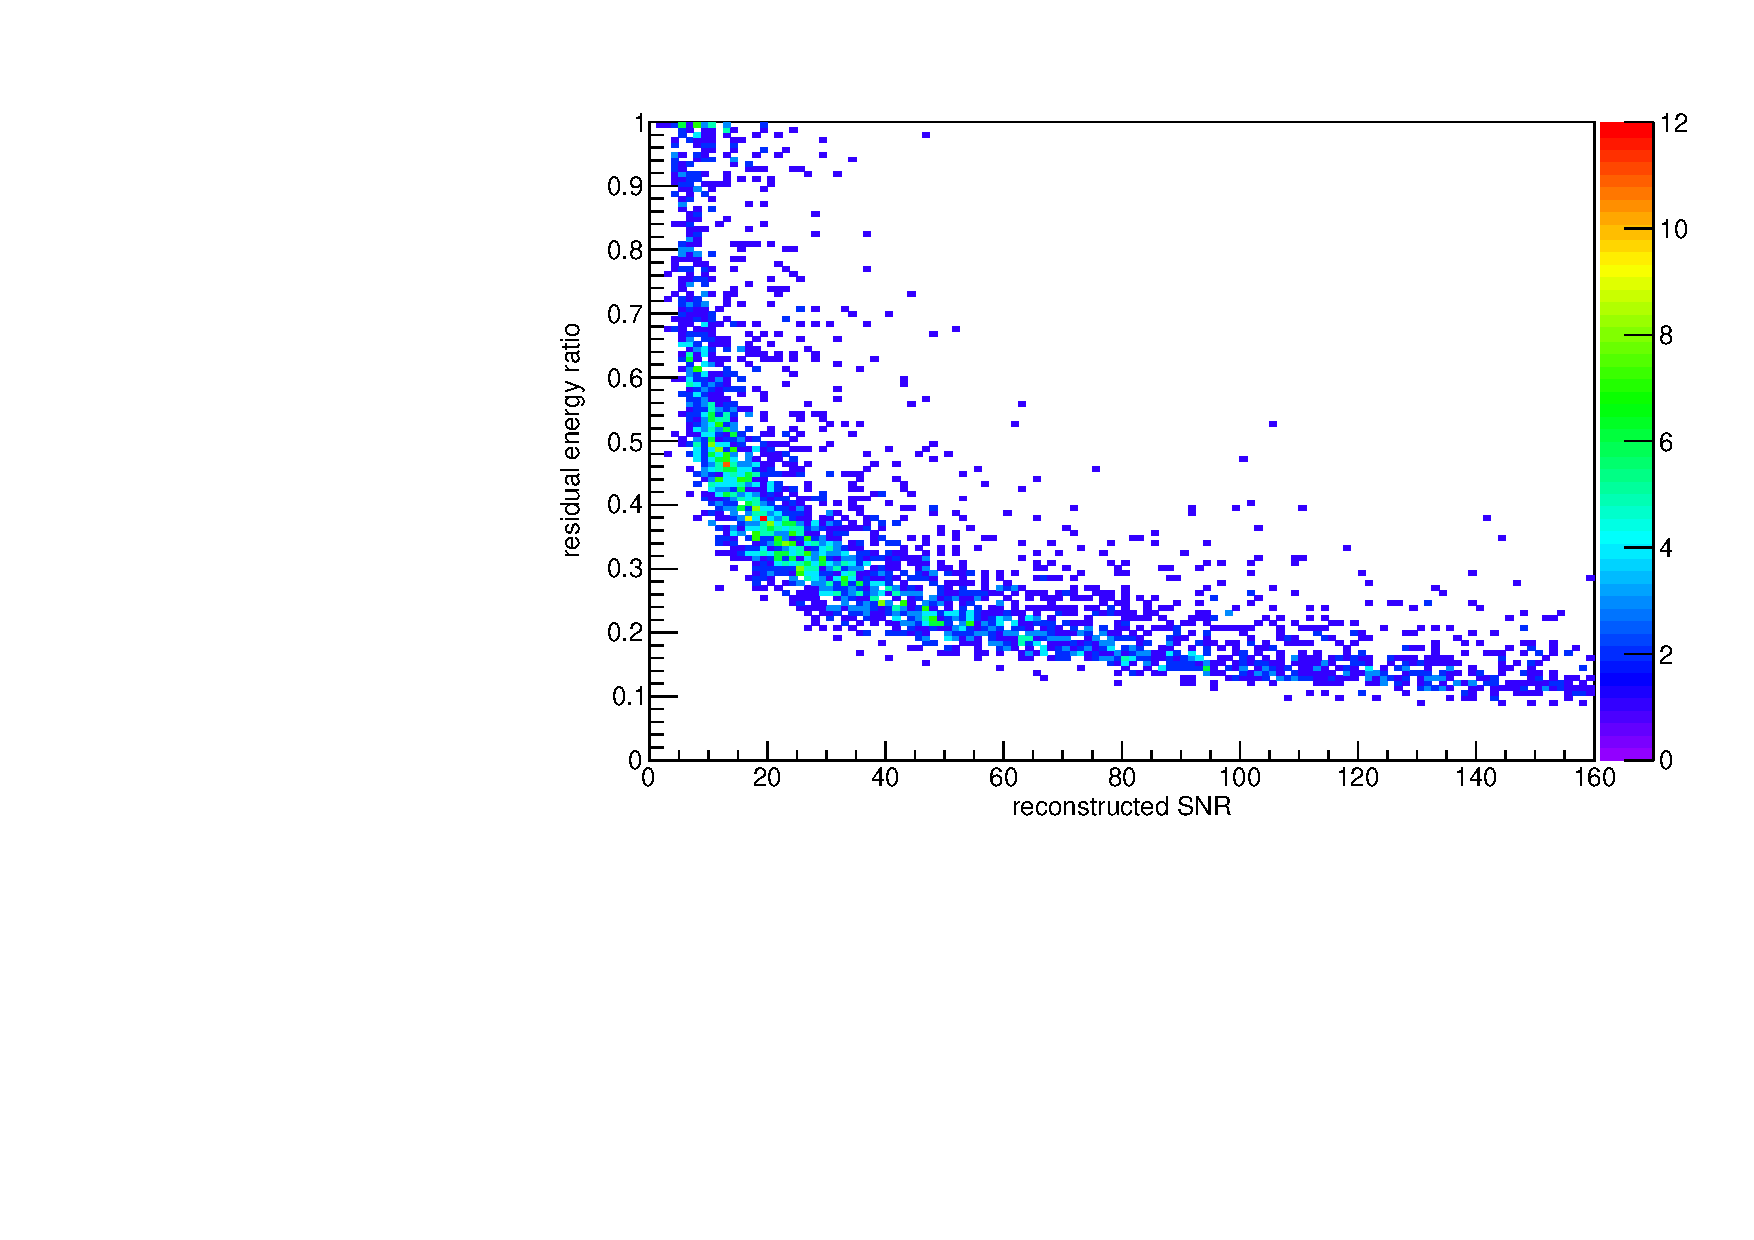
\includegraphics[width=.3333333333333\textwidth]{figures/Capitolo_3/report/RatioResidualEnergyDistributionDetector1SHT2_0spin11.pdf}}
	\subfloat[][\emph{SHT2.2}]
	{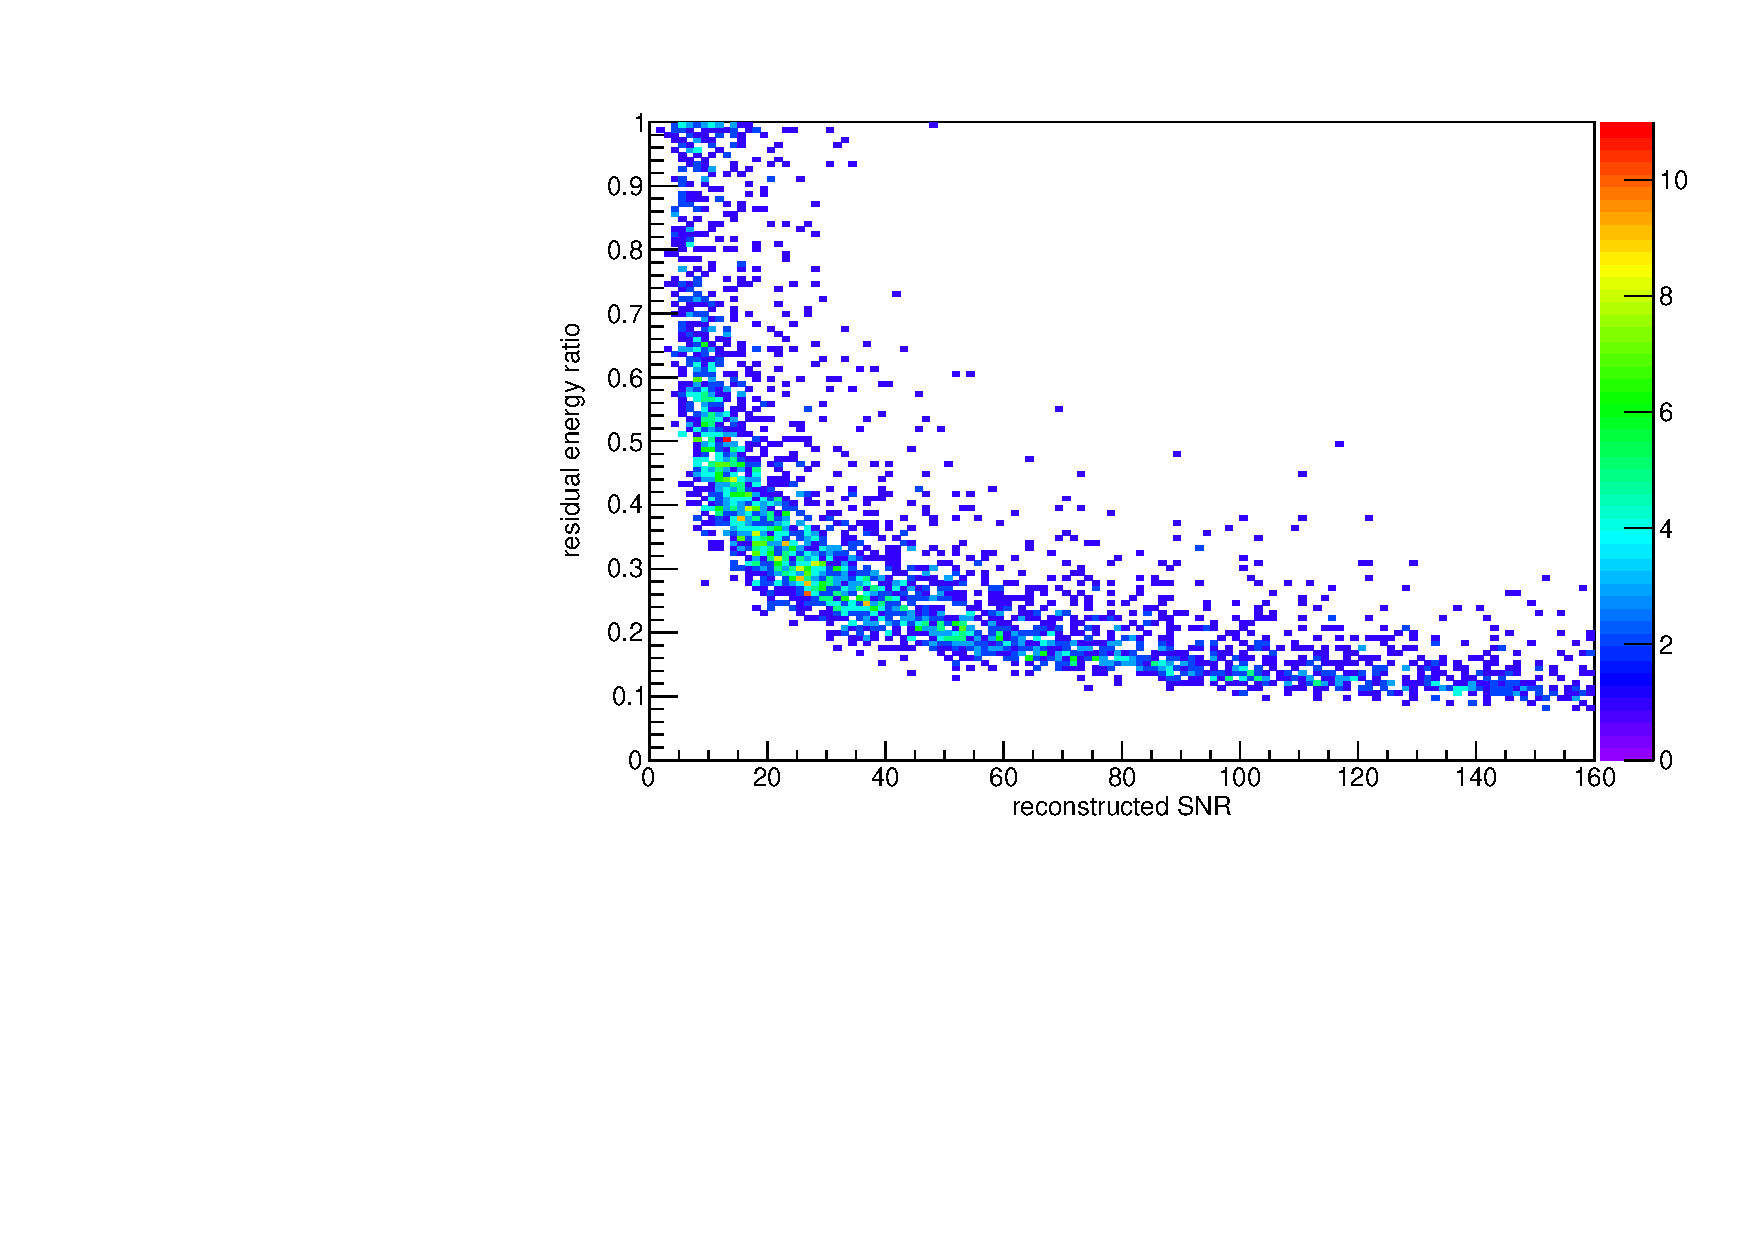
\includegraphics[width=.3333333333333\textwidth]{figures/Capitolo_3/report/RatioResidualEnergyDistributionDetector1SHT2_2spin11.pdf}}
	\subfloat[][\emph{APR4}]
	{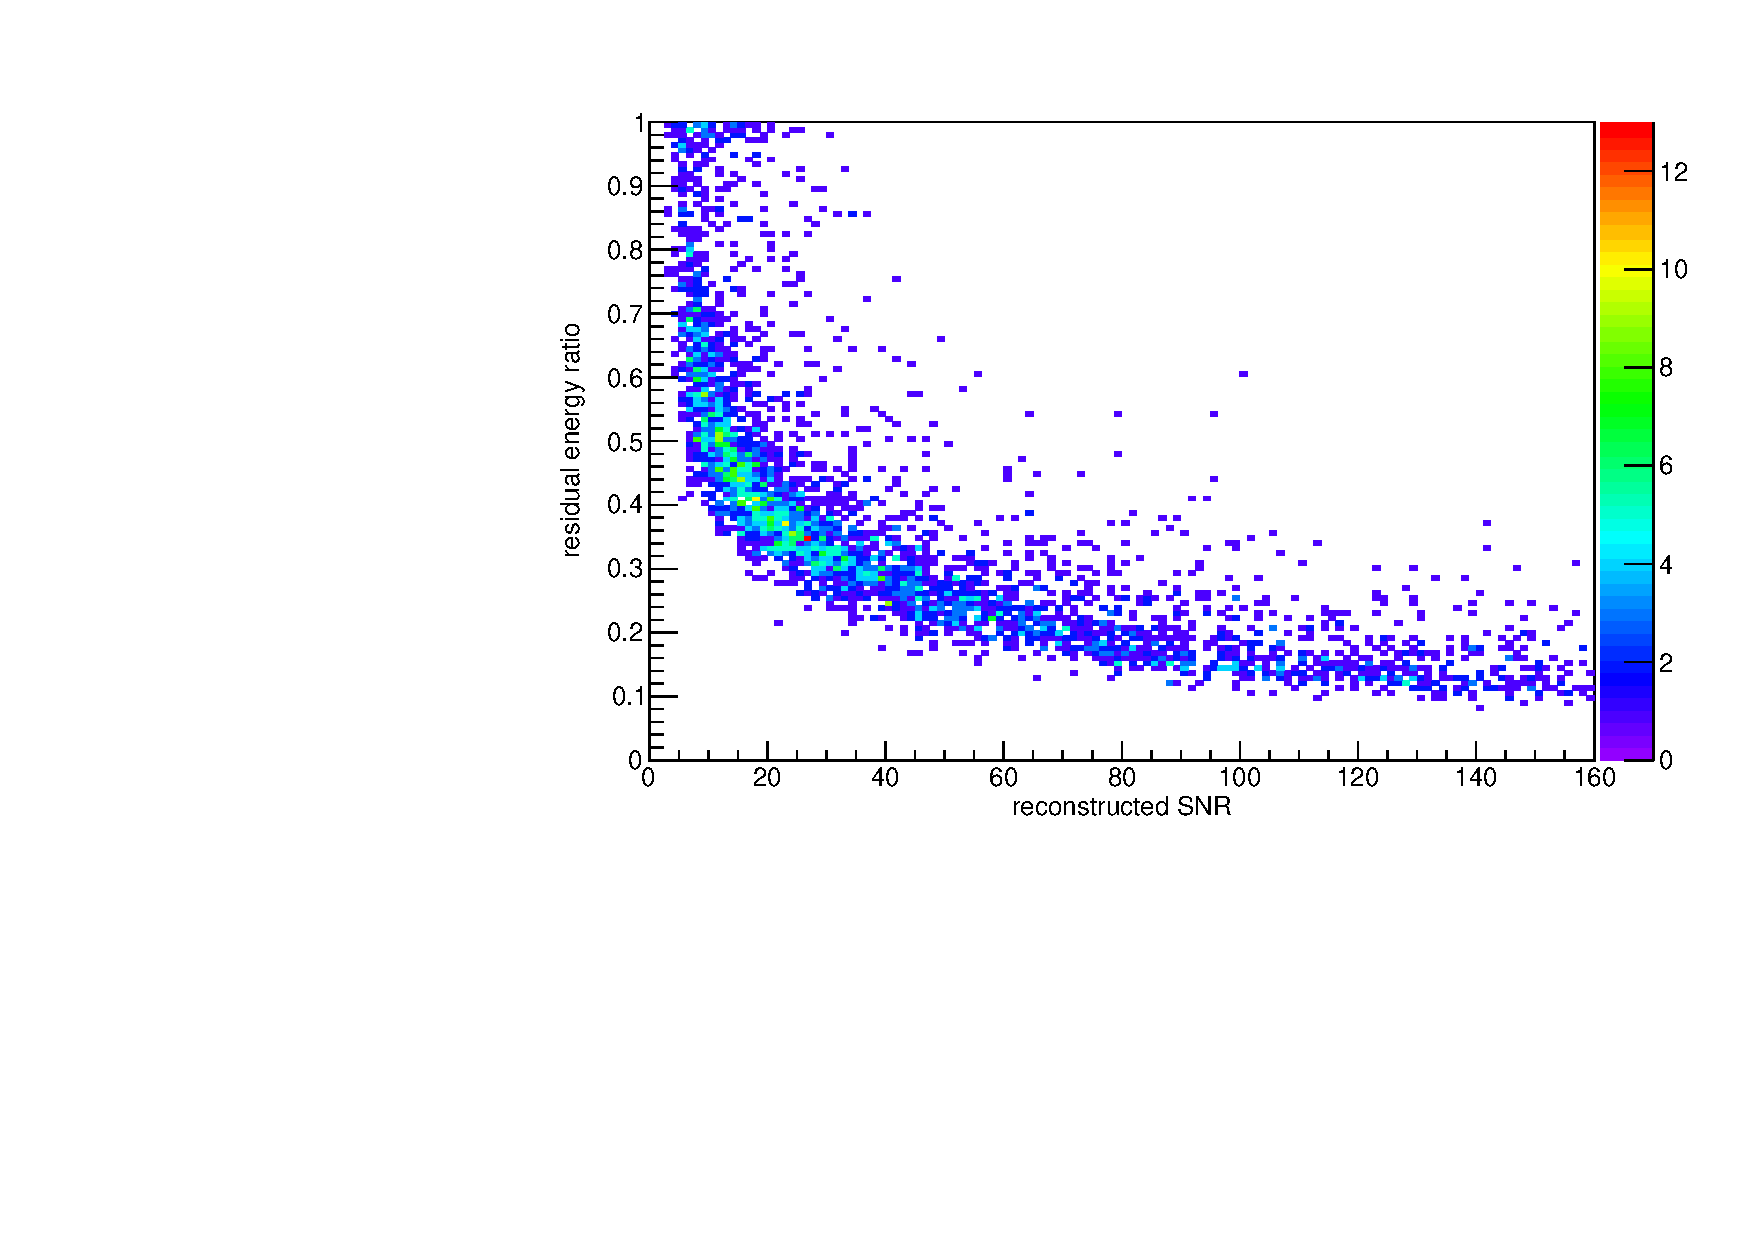
\includegraphics[width=.3333333333333\textwidth]{figures/Capitolo_3/report/RatioResidualEnergyDistributionDetector1APR4_q091.pdf}}
	\vspace{-8pt}
	\caption{Rapporto dell'energia residua rispetto all'energia totale dell'evento misurata da LIGO-Hanford}
	\label{fig:residual_energy}
	\vspace{-15pt}
\end{figure}
\begin{figure}[hbt!]
	\centering
	\subfloat[][\emph{SHT2.0 per LIGO-Hanford}]
	{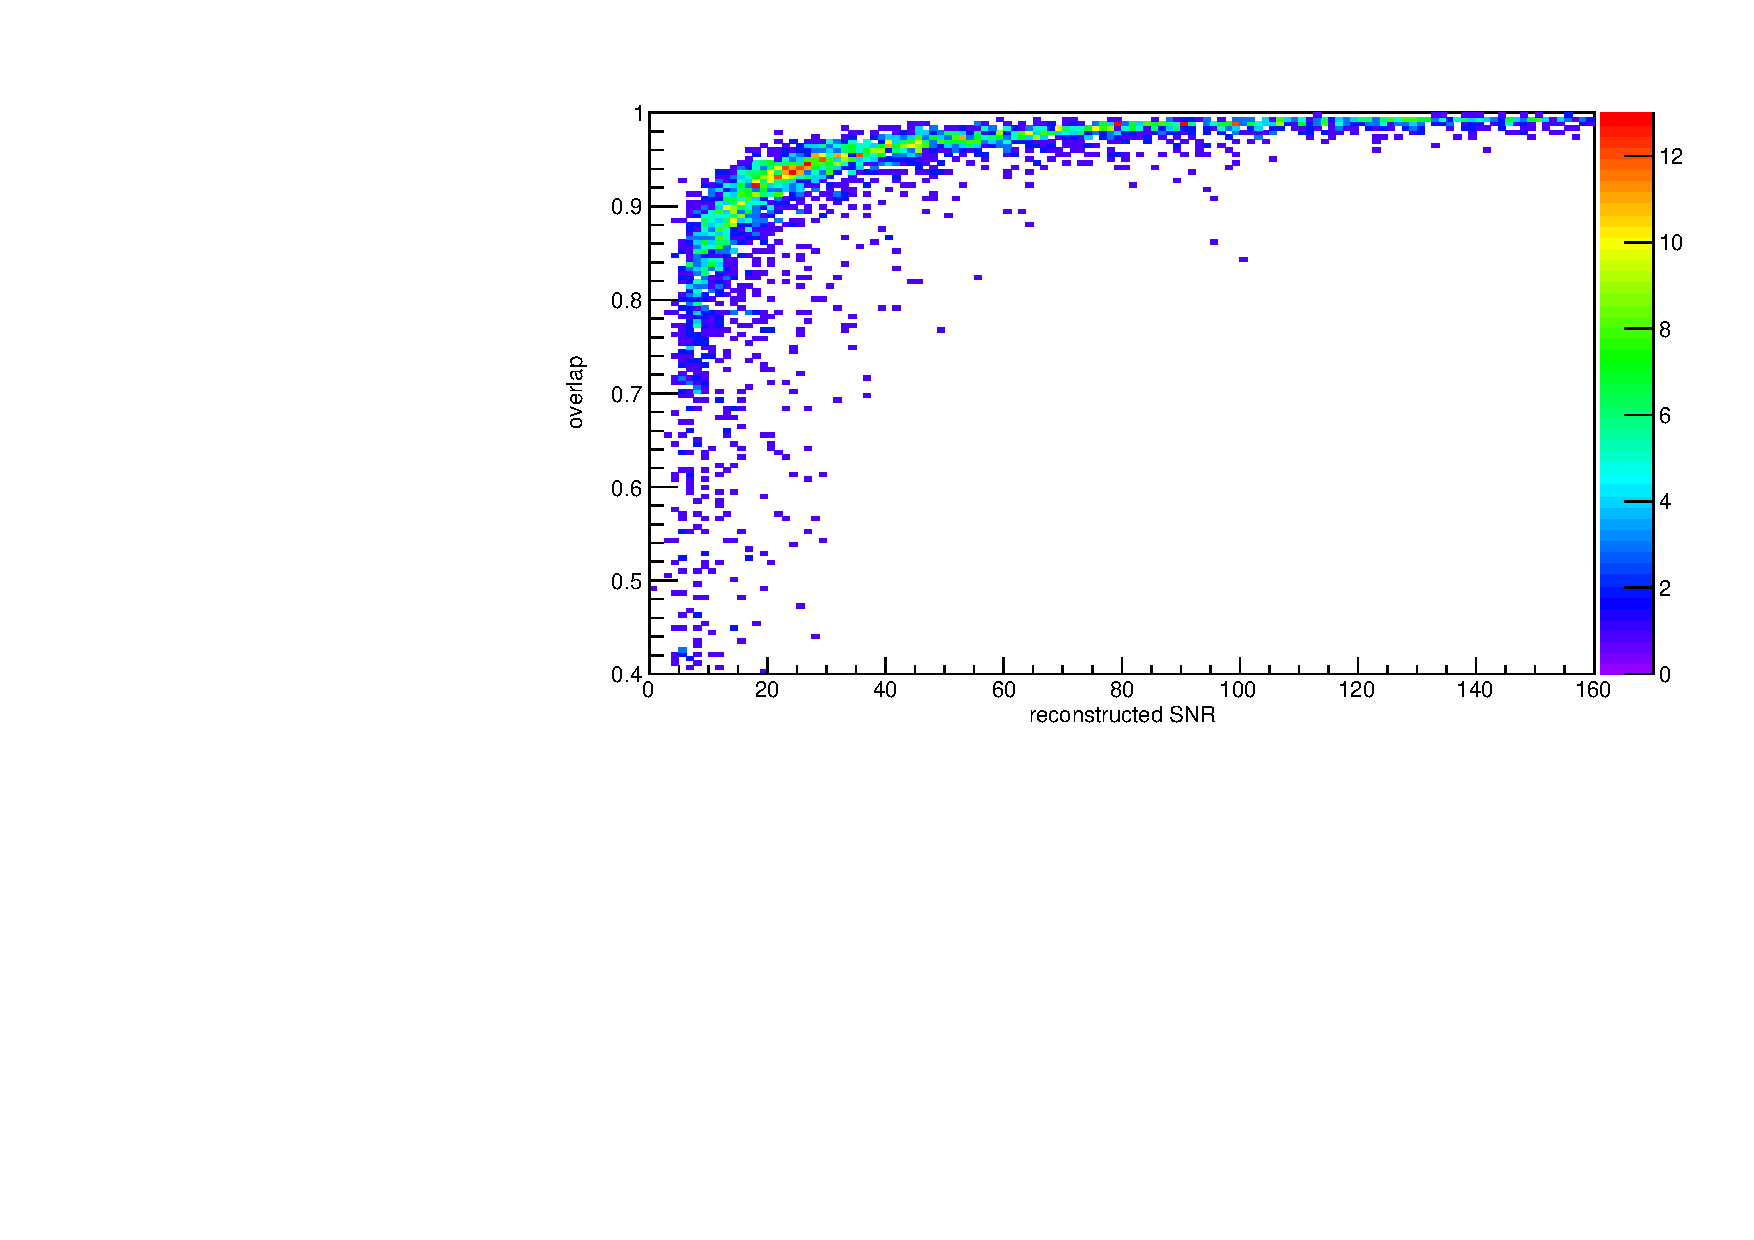
\includegraphics[width=.33\textwidth]{figures/Capitolo_3/report/OverlapDistributionDetector1APR4_q091.pdf}}
	\subfloat[][\emph{SHT2.0 per LIGO-Livingston}]
	{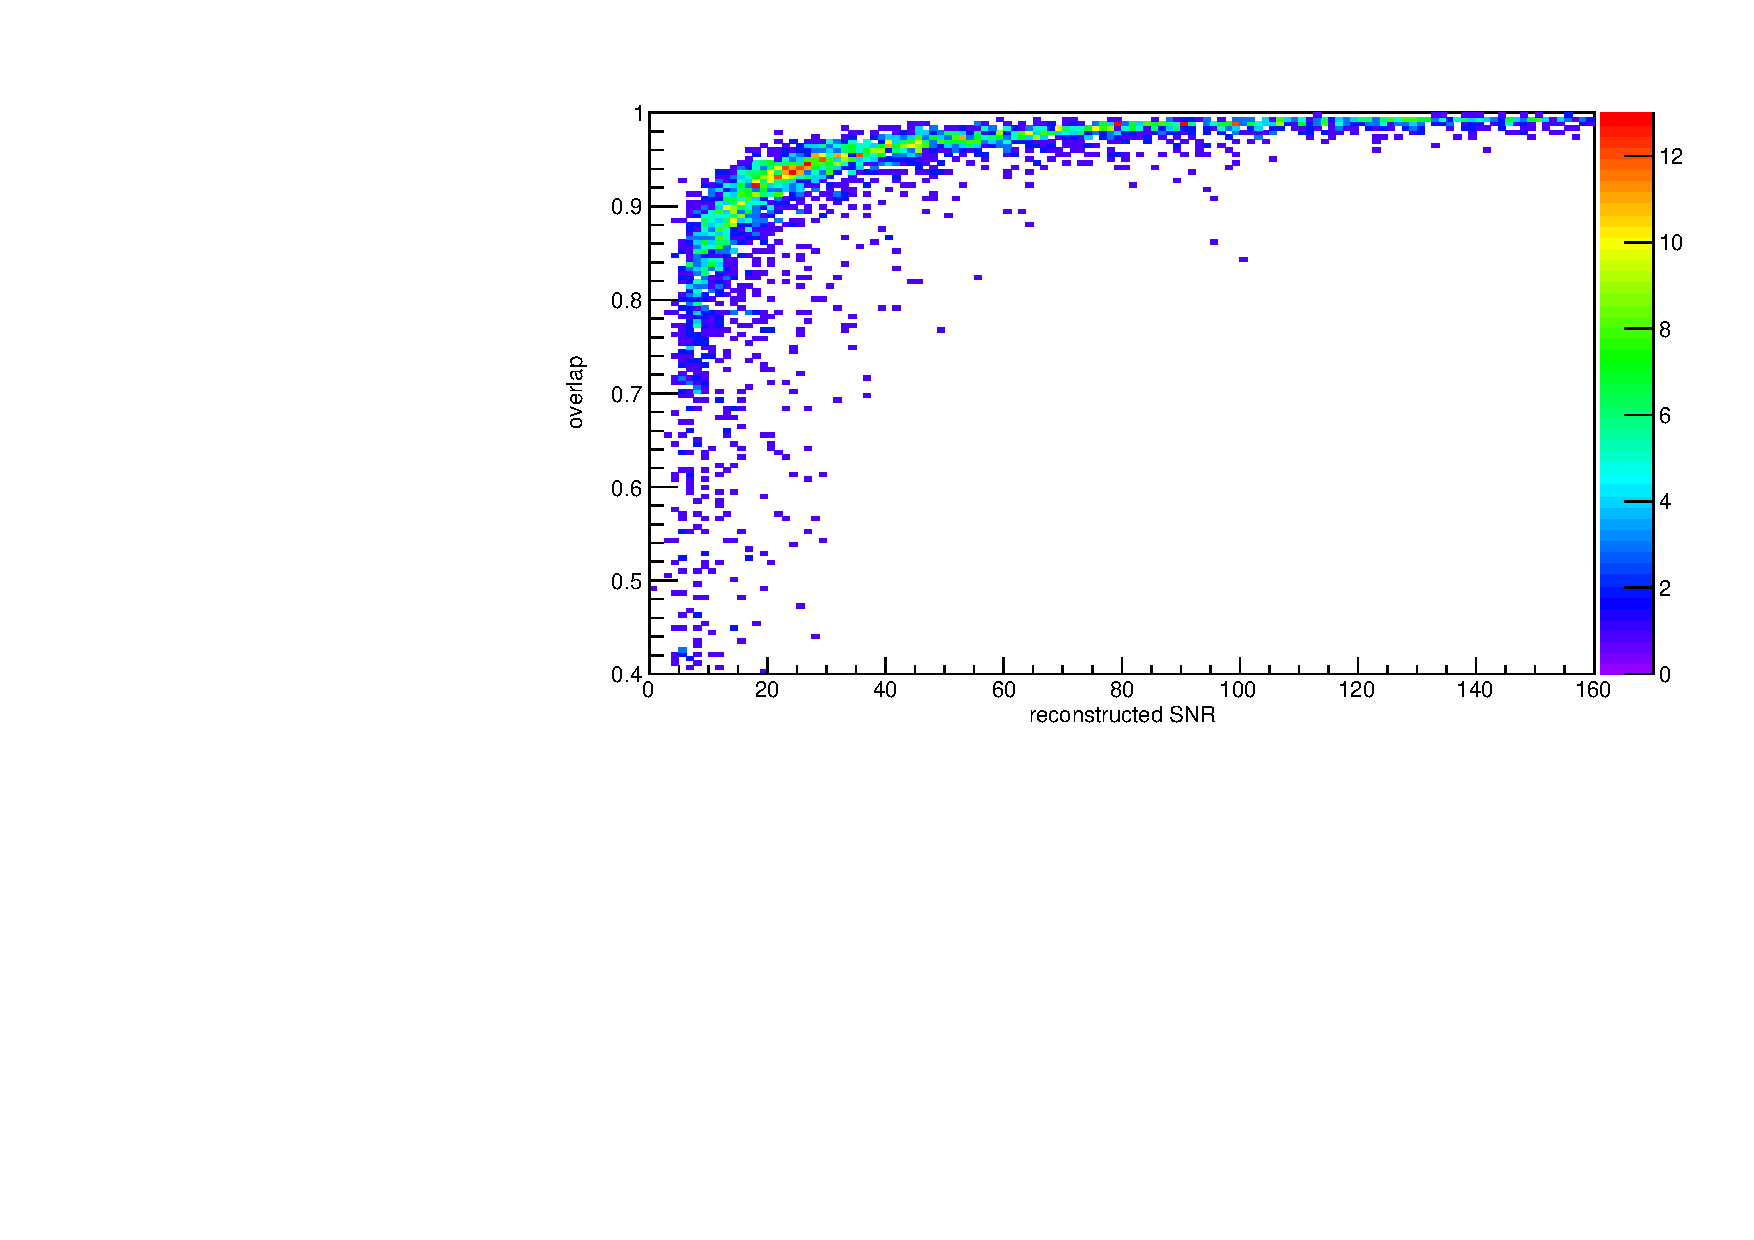
\includegraphics[width=.33\textwidth]{figures/Capitolo_3/report/OverlapDistributionDetector1APR4_q091.pdf}}
	\subfloat[][\emph{SHT2.0 per Virgo}]
	{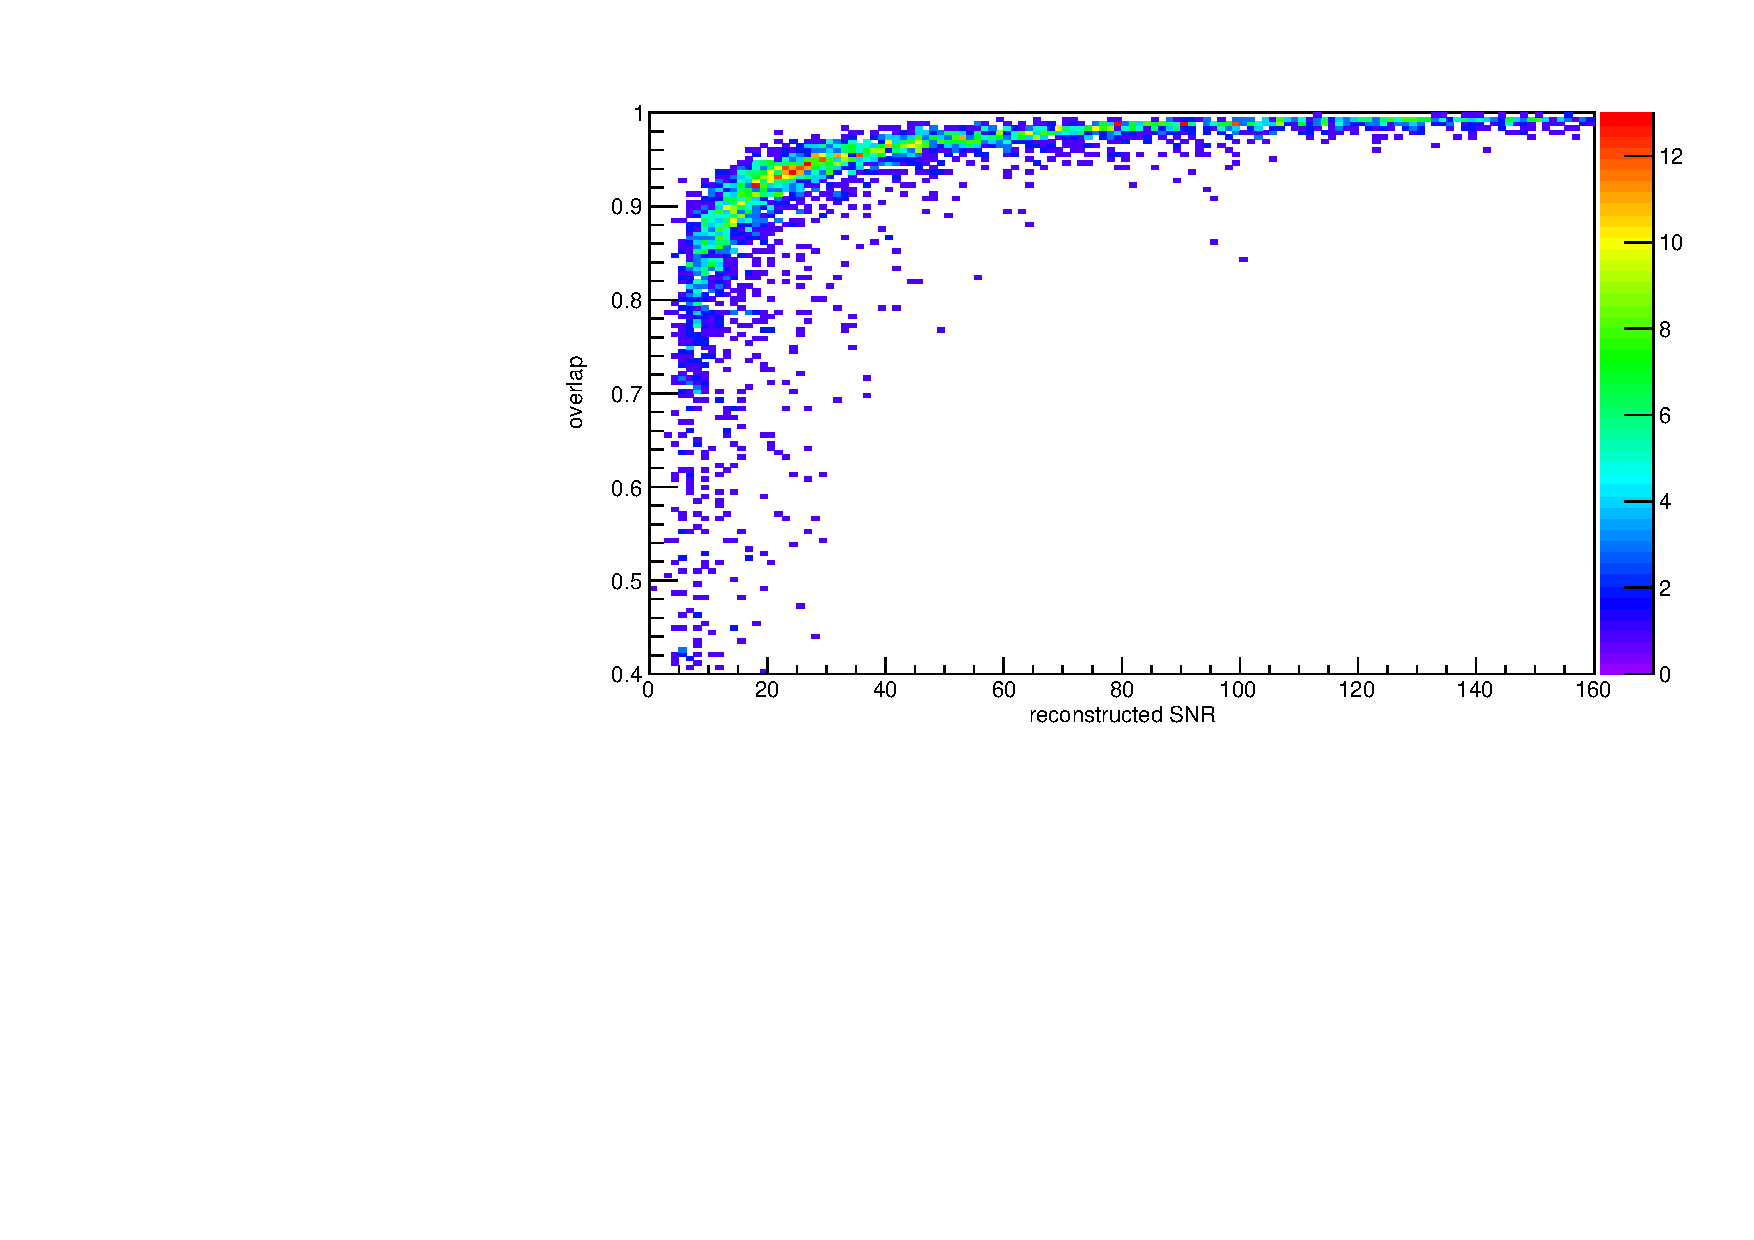
\includegraphics[width=.33\textwidth]{figures/Capitolo_3/report/OverlapDistributionDetector1APR4_q091.pdf}}
	\vspace{-8pt}
	\caption{Overlap in funzione dell'energia del rivelatore}
	\label{fig:Overlap_SHT2_APR4}
	\vspace{-5pt}
\end{figure}

\begin{wrapfigure}{r}{0.30\textwidth}
	\vspace{-20pt}
	\begin{center}
		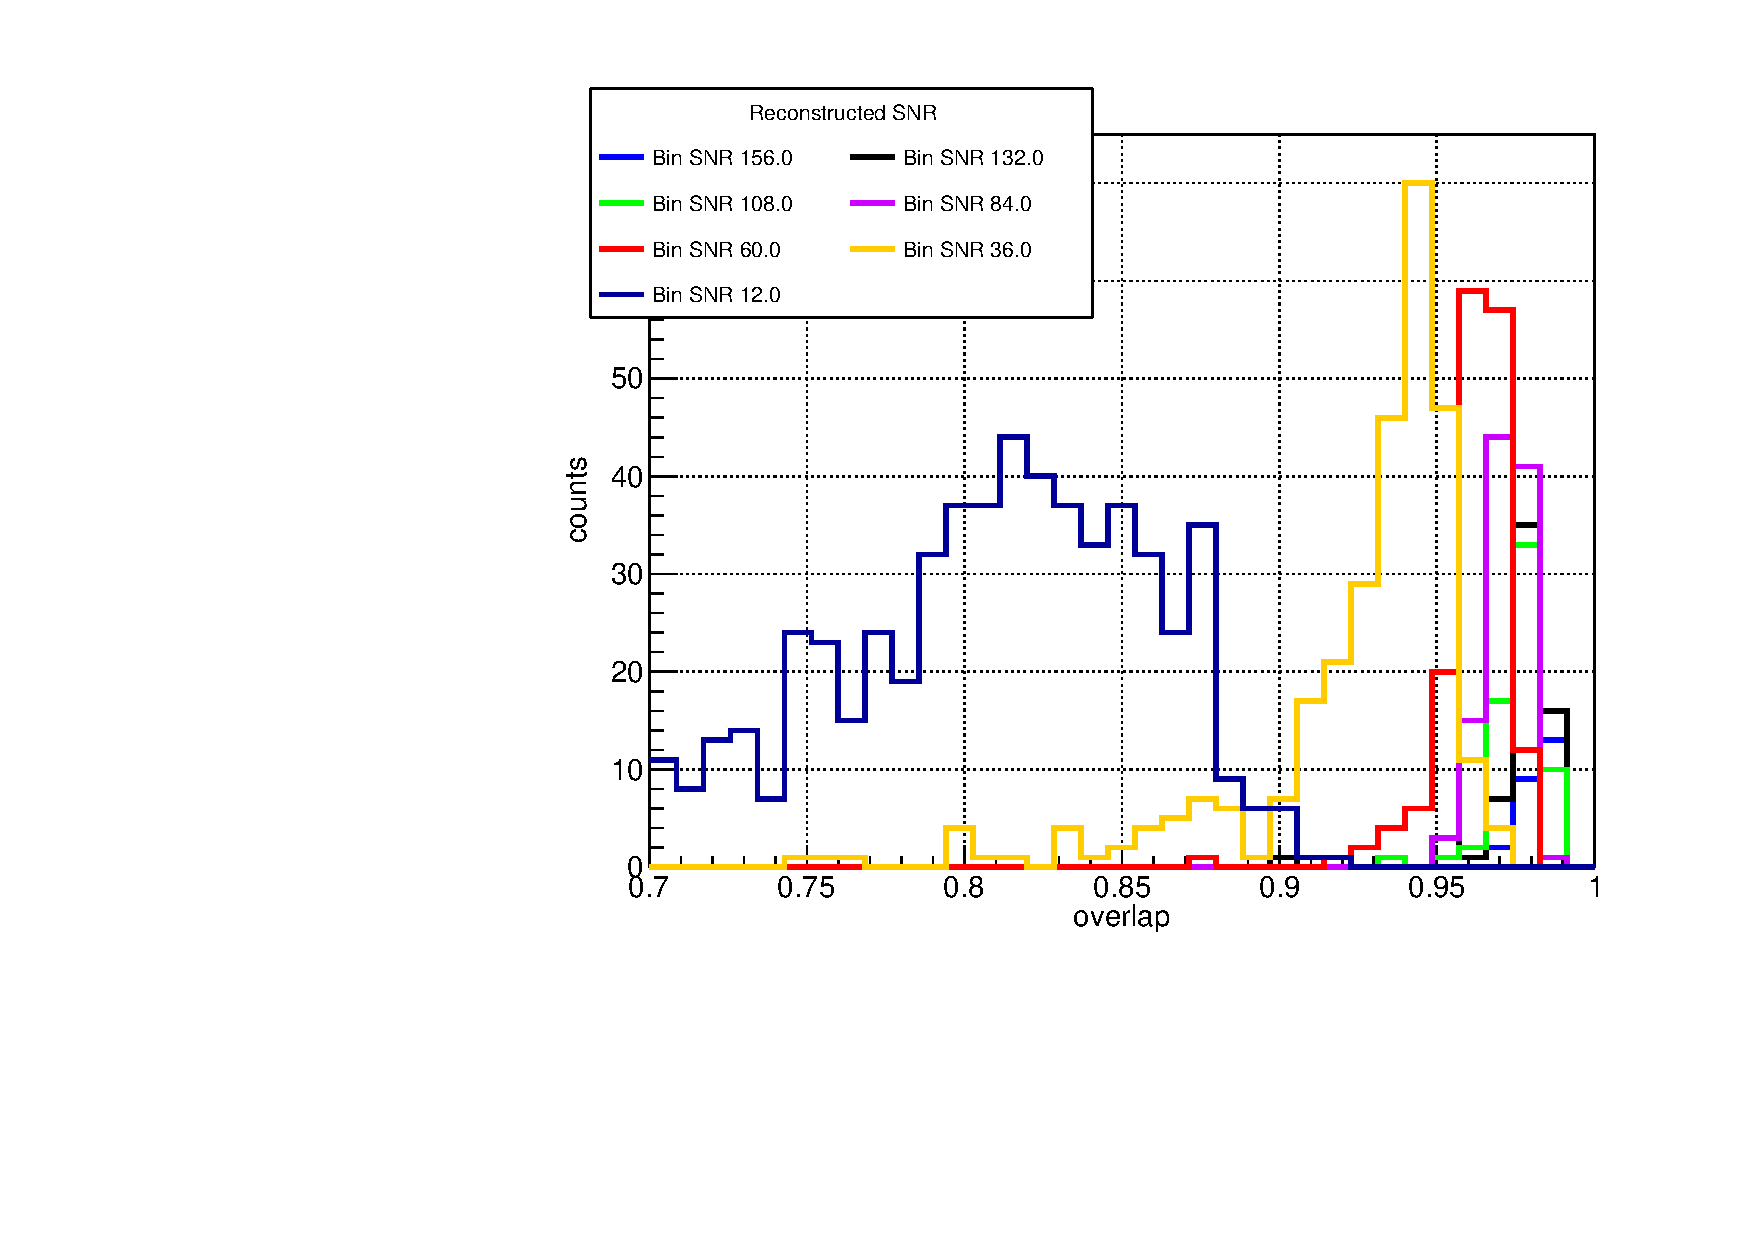
\includegraphics[width=.30\textwidth]{figures/Capitolo_3/report/OverlapDistributionsALLDetector3SHT2_0spin1.pdf}
	\end{center}
	\vspace{-12pt}
	\caption{Alcune distribuzioni degli overlap divisi per SNR ricostruito}
	\label{fig:overlaps_histo}
	\vspace{-10pt}
\end{wrapfigure}
Gli overlap sono poi stati divisi in bin di SNR ricostruito di larghezza fissata per osservare la distribuzione con la quale i segnali sono ricostruiti, che è riportata in Figura \ref{fig:overlaps_histo}, quindi viene riportato in Figura \ref{fig:Overlap_distribution} l'andamento dei valori medi, con la dispersione di ogni bin.\\
Si può notare come le ricostruzioni per Virgo risultino avere una curva di Overlap sistematicamente sottostante a quelle dei due rivelatori LIGO: questo è dovuto alla minore sensibilità di Virgo a frequenze intermedie (Fig.\ref{fig:sensitivity_O4}), dove si manifesta il contributo più energetico che è ottenuto dai rivelatori, per cui la ricostruzione di Virgo, nel contesto di uniformità della posizione celeste e della polarizzazione, sarà necessariamente peggiore.
\begin{figure}[hbt!]
	\vspace{-15pt}
	\centering
	\subfloat[][\emph{SHT2.0}]
	{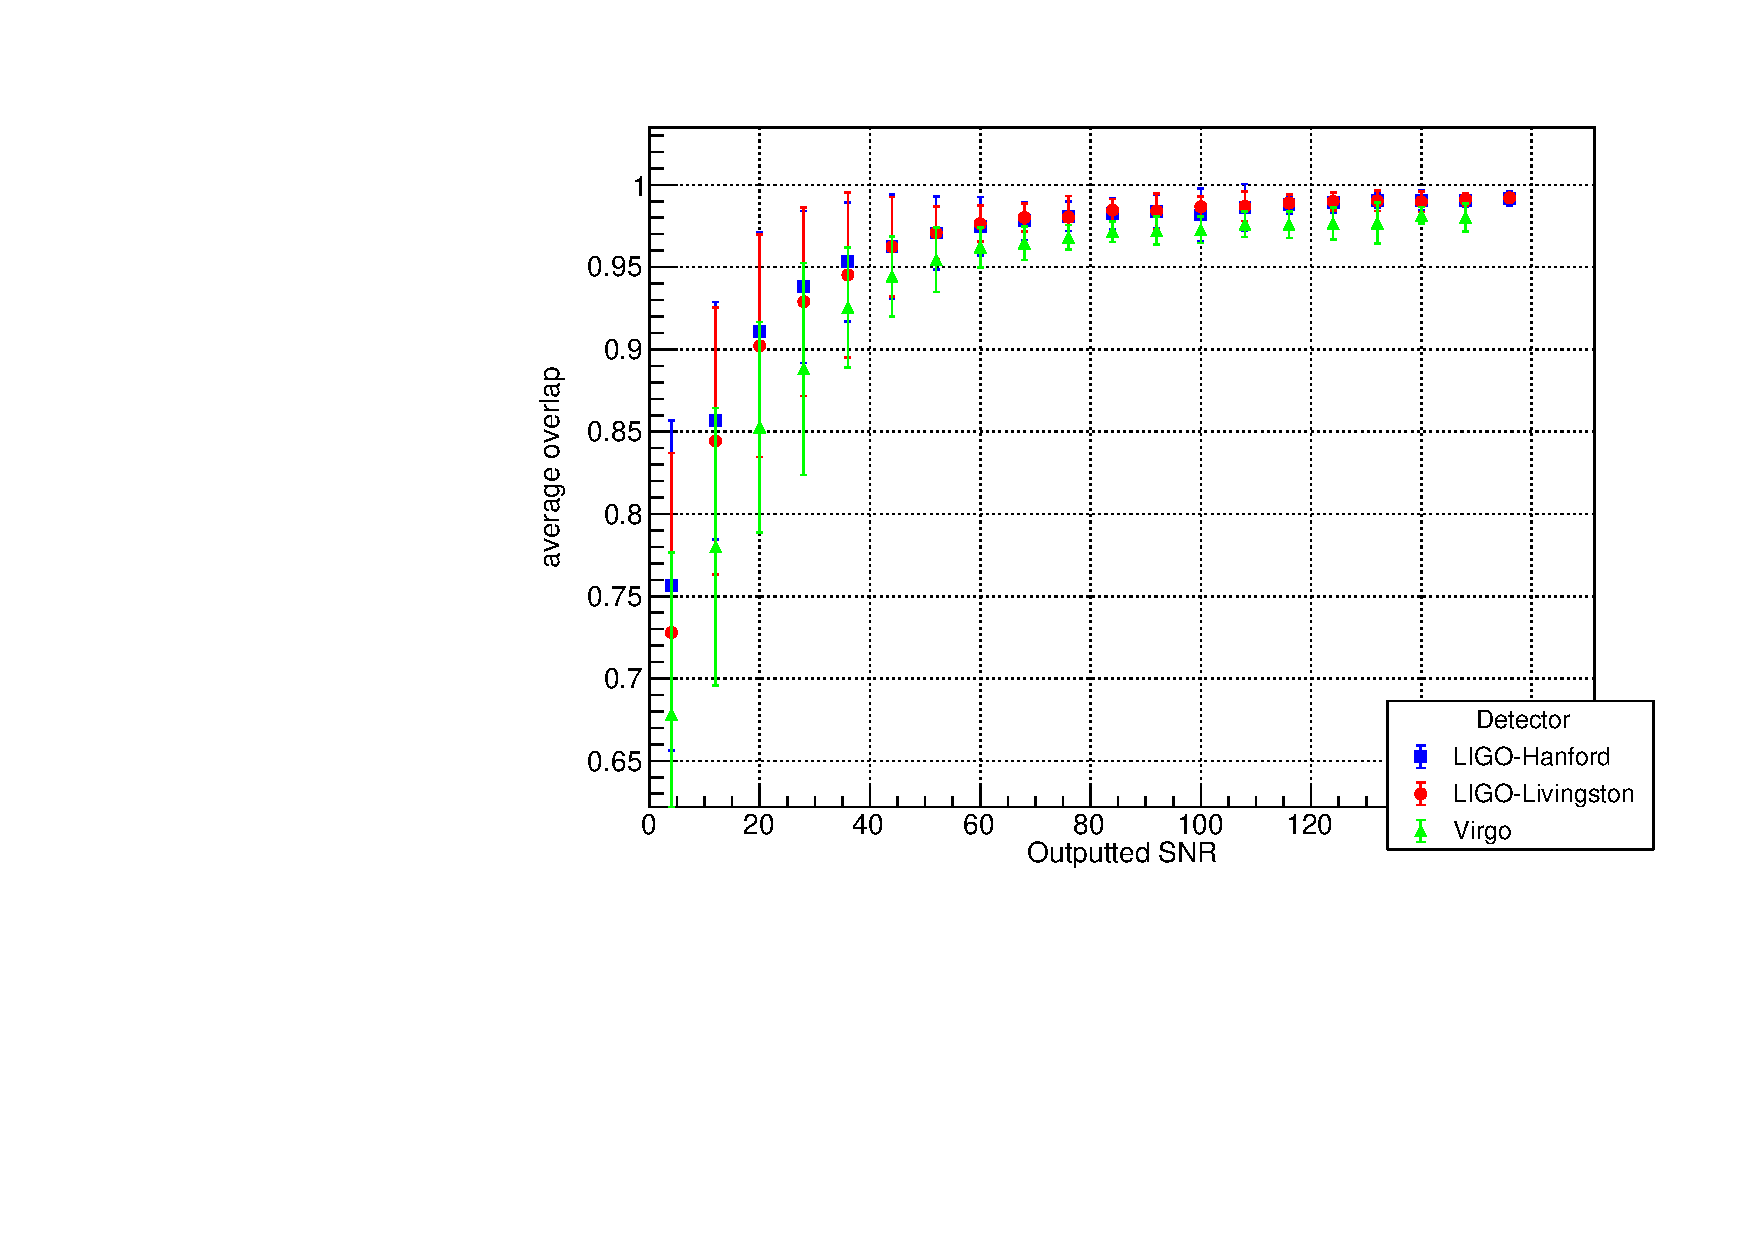
\includegraphics[width=.3333333333333333\textwidth]{figures/Capitolo_3/report/overlaps_Colors_GrapgSHT2_0spin11.pdf}}
	\subfloat[][\emph{SHT2.2}]
	{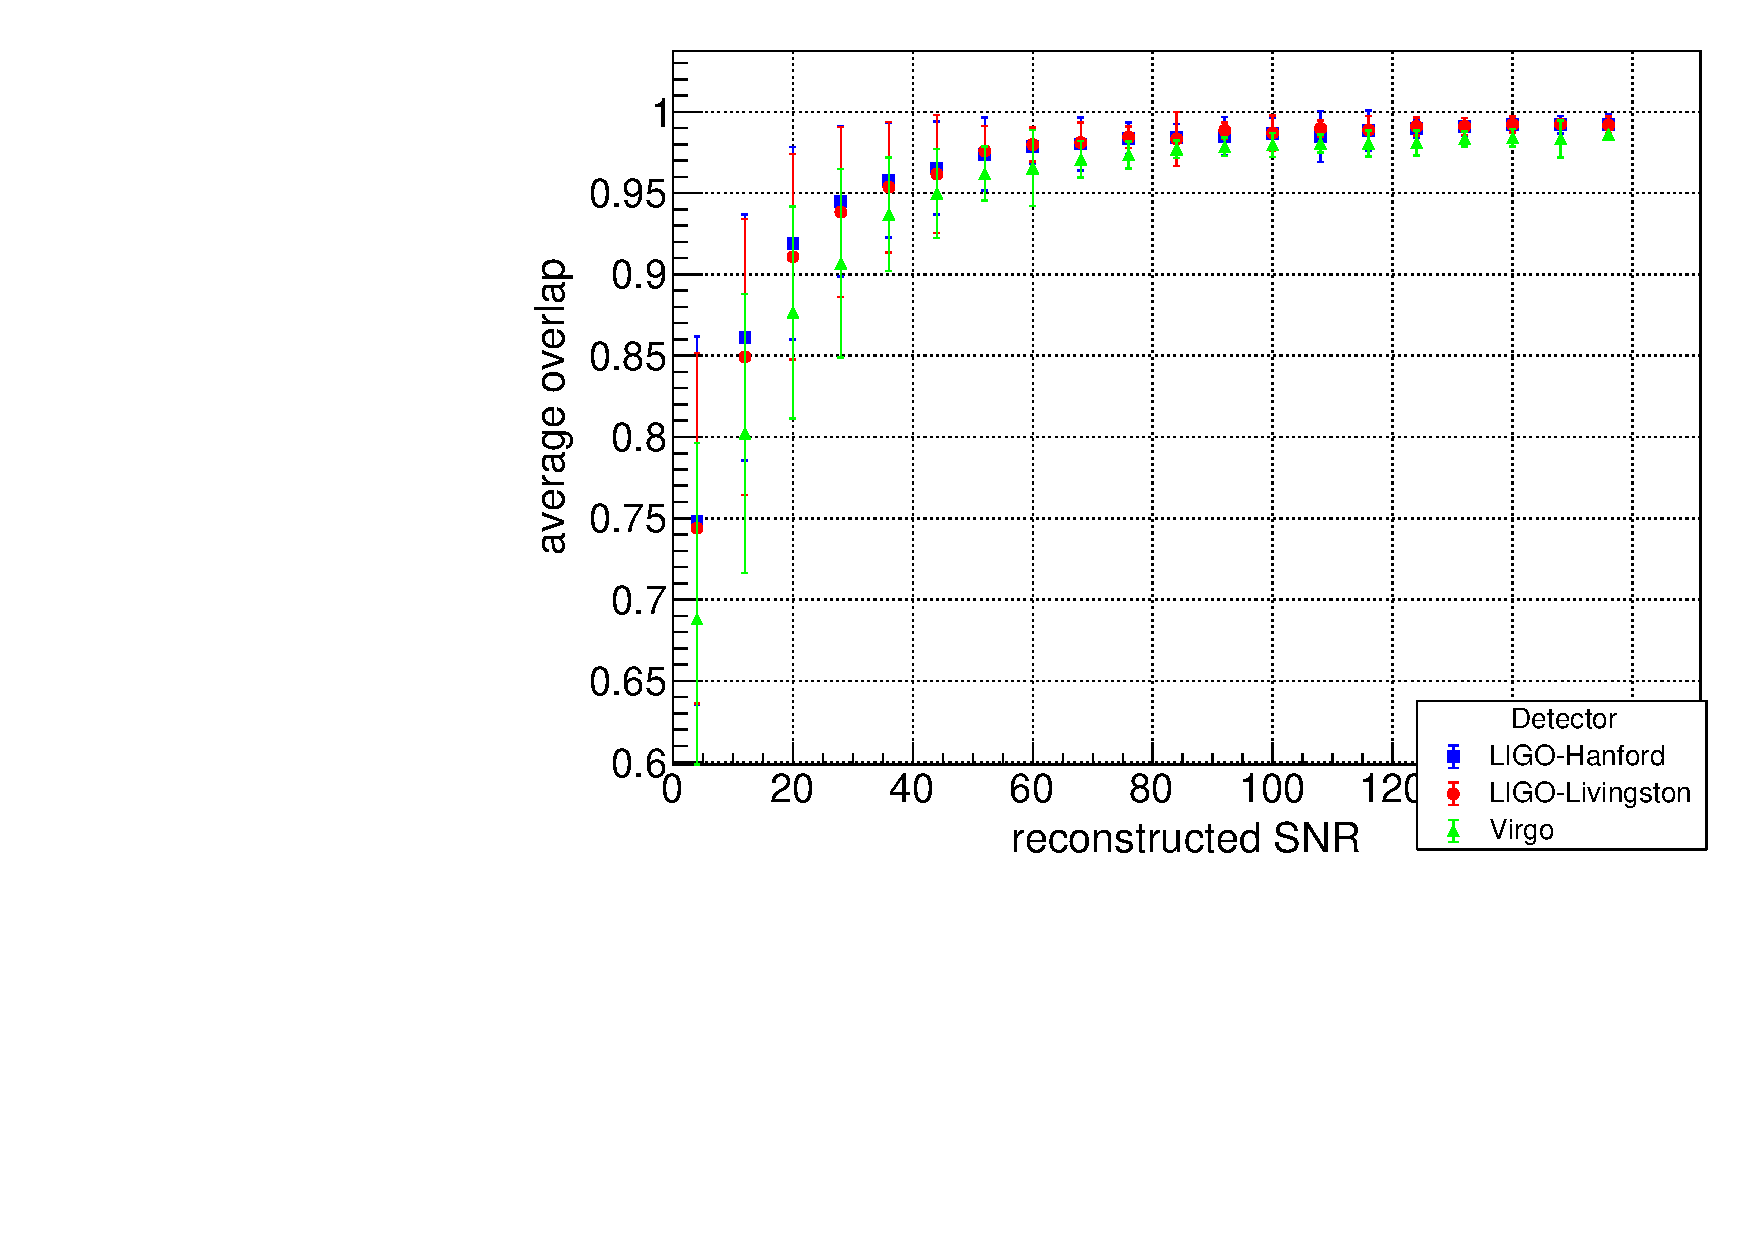
\includegraphics[width=.3333333333333333\textwidth]{figures/Capitolo_3/report/overlaps_Colors_GrapgSHT2_2spin11.pdf}}
	\subfloat[][\emph{APR4}]
	{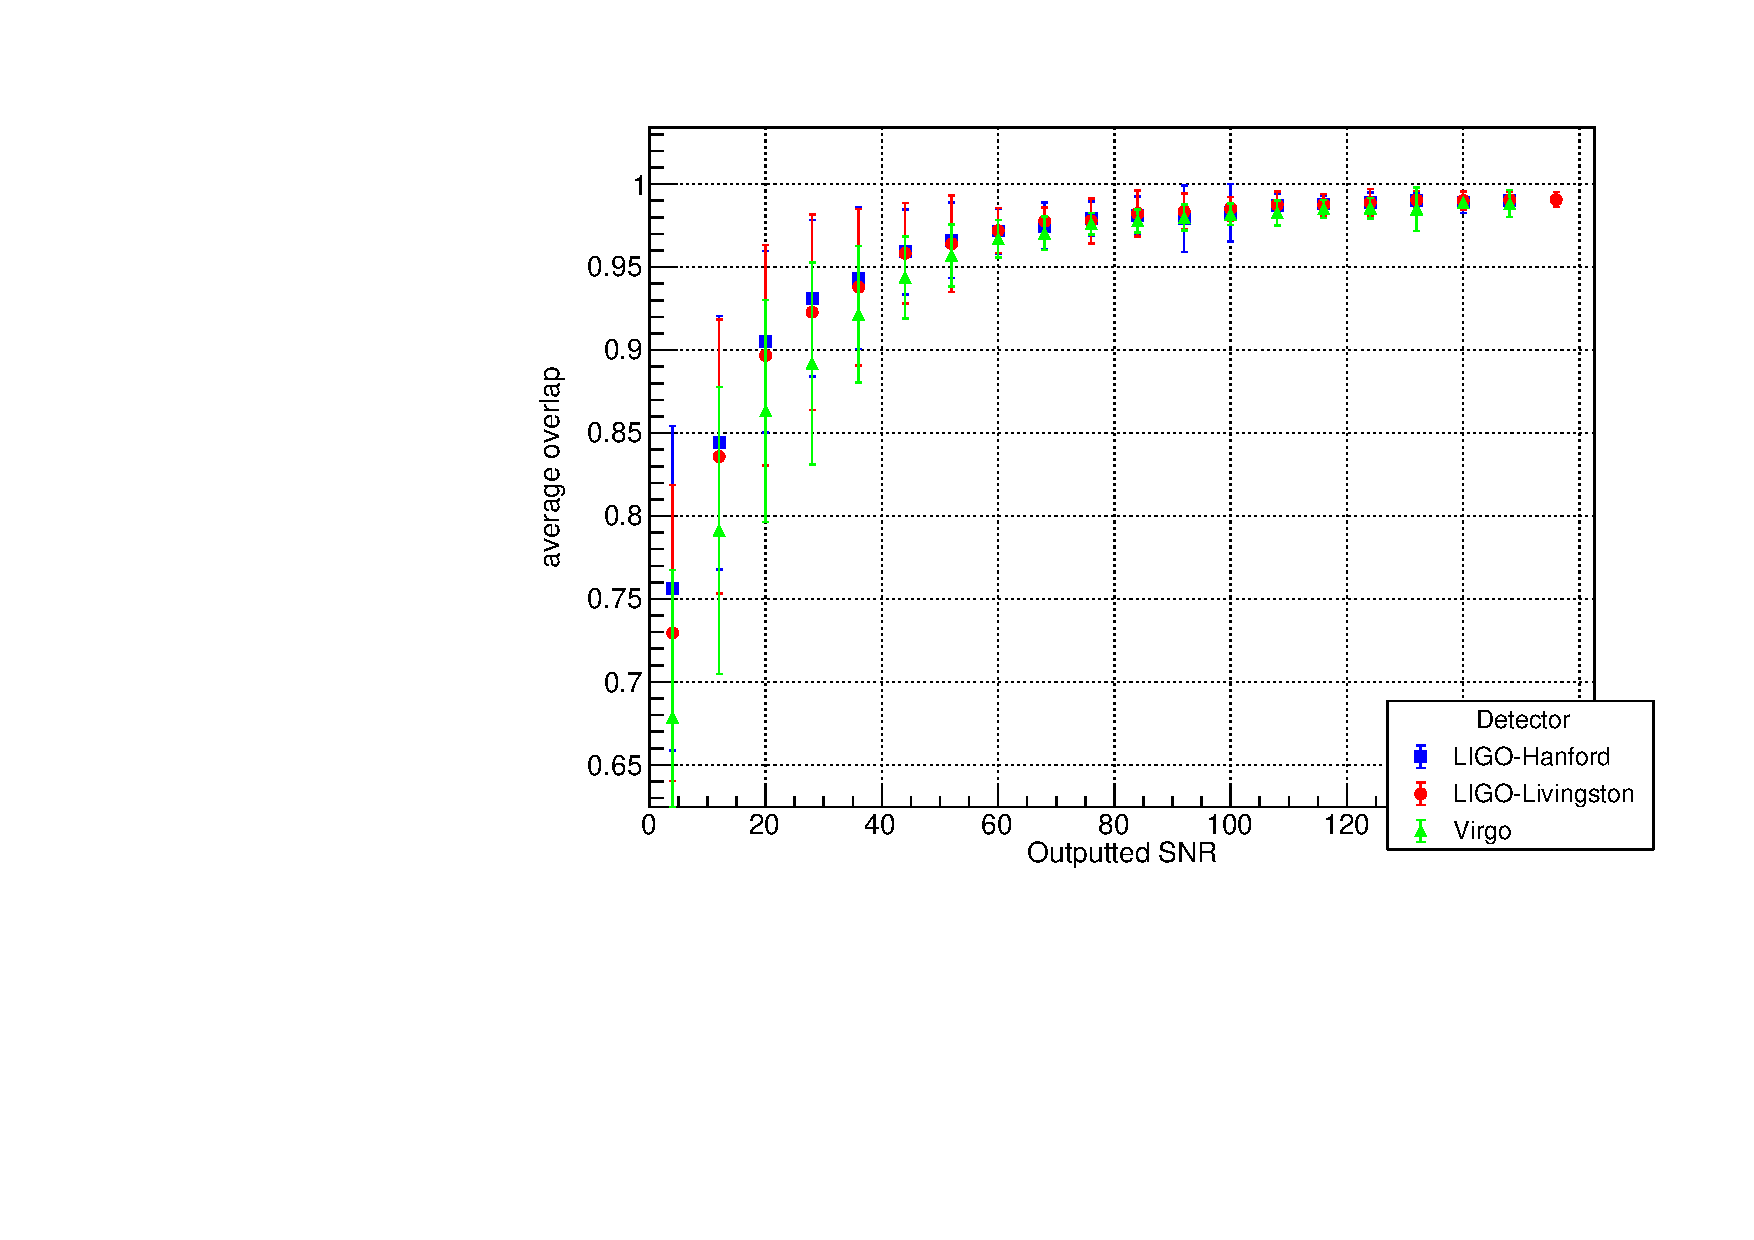
\includegraphics[width=.3333333333333333\textwidth]{figures/Capitolo_3/report/overlaps_Colors_GrapgAPR4_q091.pdf}}
	\vspace{-5pt}
	\caption{Distribuzione degli overlap per le tre EOS}
	\label{fig:Overlap_distribution}
	\vspace{-10pt}
\end{figure}
\section{Caratterizzazione della frequenza della post-coalescenza}
\label{section:Frequenza_PM}
Per valutare la frequenza della post-coalescenza del segnale ricostruito l'analisi, sviluppata in \cite{Puecher_2018} e \cite{Tringali_2017}, segue alcuni step fondamentali:
la mappa tempo-frequenza del segnale con la minima divisione in tempo, corrispondente a 1 ms, associata a una divisione in frequenza di 512 Hz, viene divisa in 4 quadranti, tagliando il piano sia in tempo che in frequenza. La risoluzione è decisa per poter studiare il segnale che si sviluppa su scale temporali estremamente ridotte, in modo da poter distinguere lo spiraleggiamento dalla post-coalescenza, che sono sono invece a frequenze molto distanti.\\
%: poiché il segnale si sviluppa su scale temporali estremamente ridotte, per poter distinguere in modo adeguato la parte finale dello spiraleggiamento e della post-coalescenza si .
%In particolare la mappa tempo-frequenza è ottenuta con una trasformazione di wavelet andando a combinare vari layer con diverse larghezze dei bin in frequenza $df$ e in tempo $dt$, definendo l'area dei pixel $df\times dt$ con energia data dall'ampiezza del pixel. Per questa analisi, 
Il taglio in frequenza è deciso in modo arbitrario in $f = 1792$Hz, comunque al di sotto della soglia di minima 2KHz. In questo modo, facendo un taglio opportuno nell'asse dei tempi, si potrà isolare il segnale di post-coalescenza e la parte finale della coalescenza nel quadrante con $t>t_{cut}$ e $f>f_{cut}$. \\ 
Per decidere l'istante di tempo in cui produrre il taglio viene fatta una media pesata con l'energia dei pixel per ogni layer
\begin{equation}
\bar{t}_j = \frac{\sum_{i=1}^Nt_{j,i}e_{i,j}}{E_{j}}
\end{equation}
dove j e i iterano sulla banda di frequenza e sul bin temporale rispettivamente, N è il numero di bin, $t_{j,i}$ e $e_{i,j}$ sono il tempo e l'energia del pixel (j, i) e infine $E_{j} = \sum_{i}e_{j,i}$ è l'energia totale del layer. Il taglio è preso quindi come $t_{cut} = \bar{t}_2 + dt$ con $\bar{t}_2$ tempo stimato per il merger, poiché quest'ultimo ha generalmente frequenze comprese tra 768Hz e 1280Hz corrispondenti al layer 2. Per gli eventi con SNR ricostruito limitato, non avendo segnale nella seconda banda in frequenza, il tempo per il taglio è preso a $t_{cut} = \bar{t}_1 + 5dt$. \\
Per dare una stima di frequenza e larghezza di banda della post-coalescenza pesate con l'energia si produce nuovamente la mappa tempo-frequenza del segnale con una migliore risoluzione in frequenza $df=64$Hz. Il taglio precedente nel dominio dei tempi rimane valido, cambia invece il taglio nel dominio delle frequenze che è preso questa volta a $f_{cut}' = 1760$Hz. Un esempio viene riportato in Figura \ref{fig:time_freq_pm}.\\
La frequenza pesata, il parametro che si utilizzerà, è quindi calcolata come 
\begin{equation}
f_w=\frac{\sum_{i,j}f_{i,j}e_{i,j}}{\sum_{i,j}e_{i,j}}
\end{equation}
con $f_{i,j}$ frequenza del pixel $[i,j]$ presa come frequenza centrale del layer al quale il pixel appartiene. È calcolata inoltre anche la larghezza di banda pesata, che è definita come la varianza pesata  della frequenza
\begin{equation}
b_w =\frac{\sum_{i=1}^Nf_{c,i}^2e_i}{\sum_{i=1}^Ne_i} - \left(\ \frac{\sum_{i=1}^Nf_{c,i}e_i}{\sum_{i=1}^Ne_i}\right)^2
\end{equation}
Si osserva comunque che questo metodo non è ottimale, andando a raccogliere anche parte della fine dello spiraleggiamento portando a una sottostima sistematica della frequenza.
\begin{figure}[hbt!]
	\vspace{-20pt}
	\centering
	\subfloat[][\emph{Segnale completo}]
	{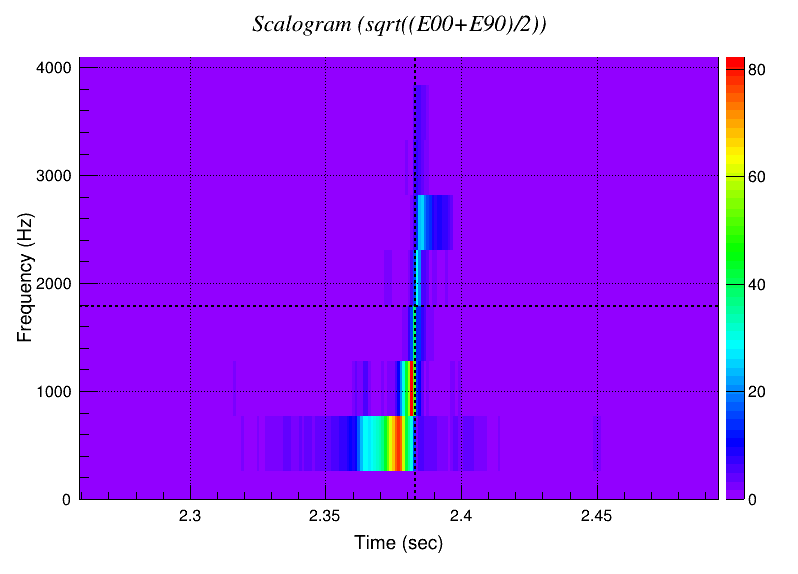
\includegraphics[width=.4\textwidth]{figures/Capitolo_3/dump/1/wdm_296_2_layers64_recPM2.png}}\quad\quad
	\subfloat[][\emph{Segnale post-coalescenza}]
	{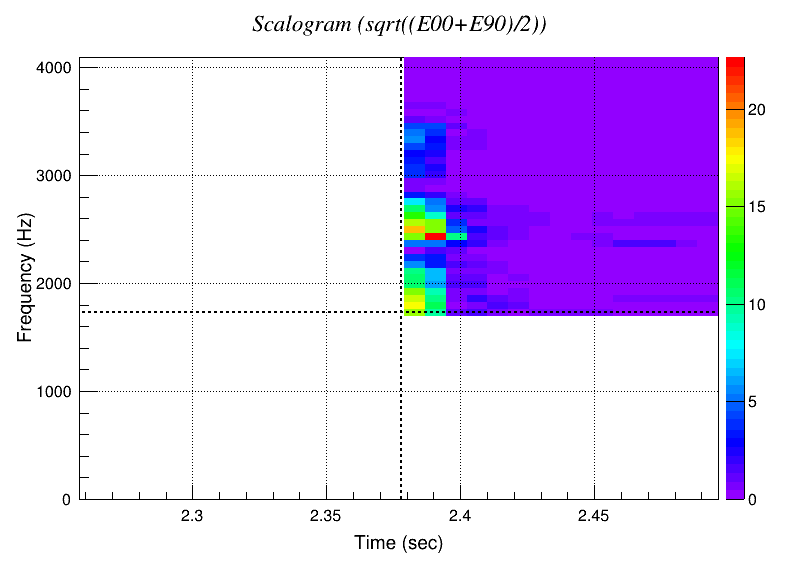
\includegraphics[width=.4\textwidth]{figures/Capitolo_3/dump/1/wdm64_296_2_layers64_recPM2.png}}
	\vspace{-8pt}
	\caption{Mappe tempo-frequenza del segnale per Virgo, a sinistra segnale ricostruito con la divisione temporale più precisa, a destra il segnale isolato con divisione $df = 64$Hz}
	\label{fig:time_freq_pm}
	\vspace{-8pt}
\end{figure}

\begin{wrapfigure}{r}{0.45\textwidth}
	\vspace{-10pt}
	\begin{center}
		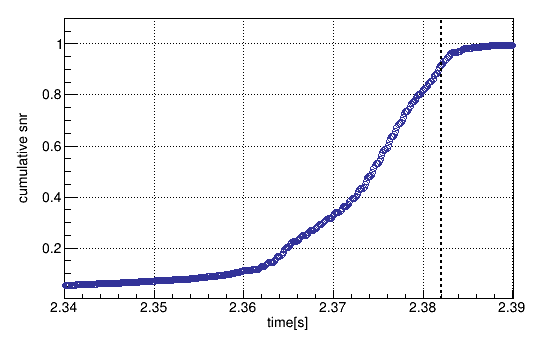
\includegraphics[width=0.45\textwidth]{figures/Capitolo_3/dump/1/V1_snr_cum_SHTdfdt_296.png}
	\end{center}
	\vspace{-8pt}
	\caption{SNR cumulativo}
	\label{fig:snr_cum}
	\vspace{-10pt}
\end{wrapfigure}
È poi interessante valutare il peso relativo del segnale di post coalescenza all'energia ricostruita, rispetto al segnale complessivo. Per fare questo è utile mostrare l'SNR cumulativo in funzione del tempo, in Figura \ref{fig:snr_cum}, si può notare come il contributo della post-coalescenza risulti estremamente ridotto in rapporto alla fase di spiraleggiamento, a prova dell'estrema difficoltà nel rivelare questa fase del segnale.

Questo procedimento è stato fatto, come per l'analisi precedente, sistematicamente su un grande numero di eventi ricostruiti in modo da poterne valutare l'efficienza e studiare i risultati. Si riporta in Figura \ref{fig:energy_pm_colz} l'energia stimata per il segnale di post-coalescenza, in funzione dell'energia totale per le diverse distanze: è facile intuire che per gli eventi a distanza maggiore il segnale di post-coalescenza viene rivelato in casi molto limitati, mentre per distanze minori verrano ricostruiti più segnali.\\
Si osserva inoltre che per la EOS SHT2.2, in cui non è atteso alcun segnale di post-coalescenza, poiché come si osserva in Figura \ref{fig:forme_onda} il sistema ha un ringdown e non c'è emissione di segnali dopo la coaelescenza, si registra energia significativa anche nella post-coalescenza. Questo risulta quindi un importante limite del metodo utilizzato: non permette di distinguere segnali con e senza post-coalescenza. Si osserva comunque che gli eventi ricostruiti sono meno numerosi e meno energetici.
\begin{figure}[hbt!]
	\vspace{-15pt}
	\centering
	\subfloat[][\emph{SHT2\_0}]
	{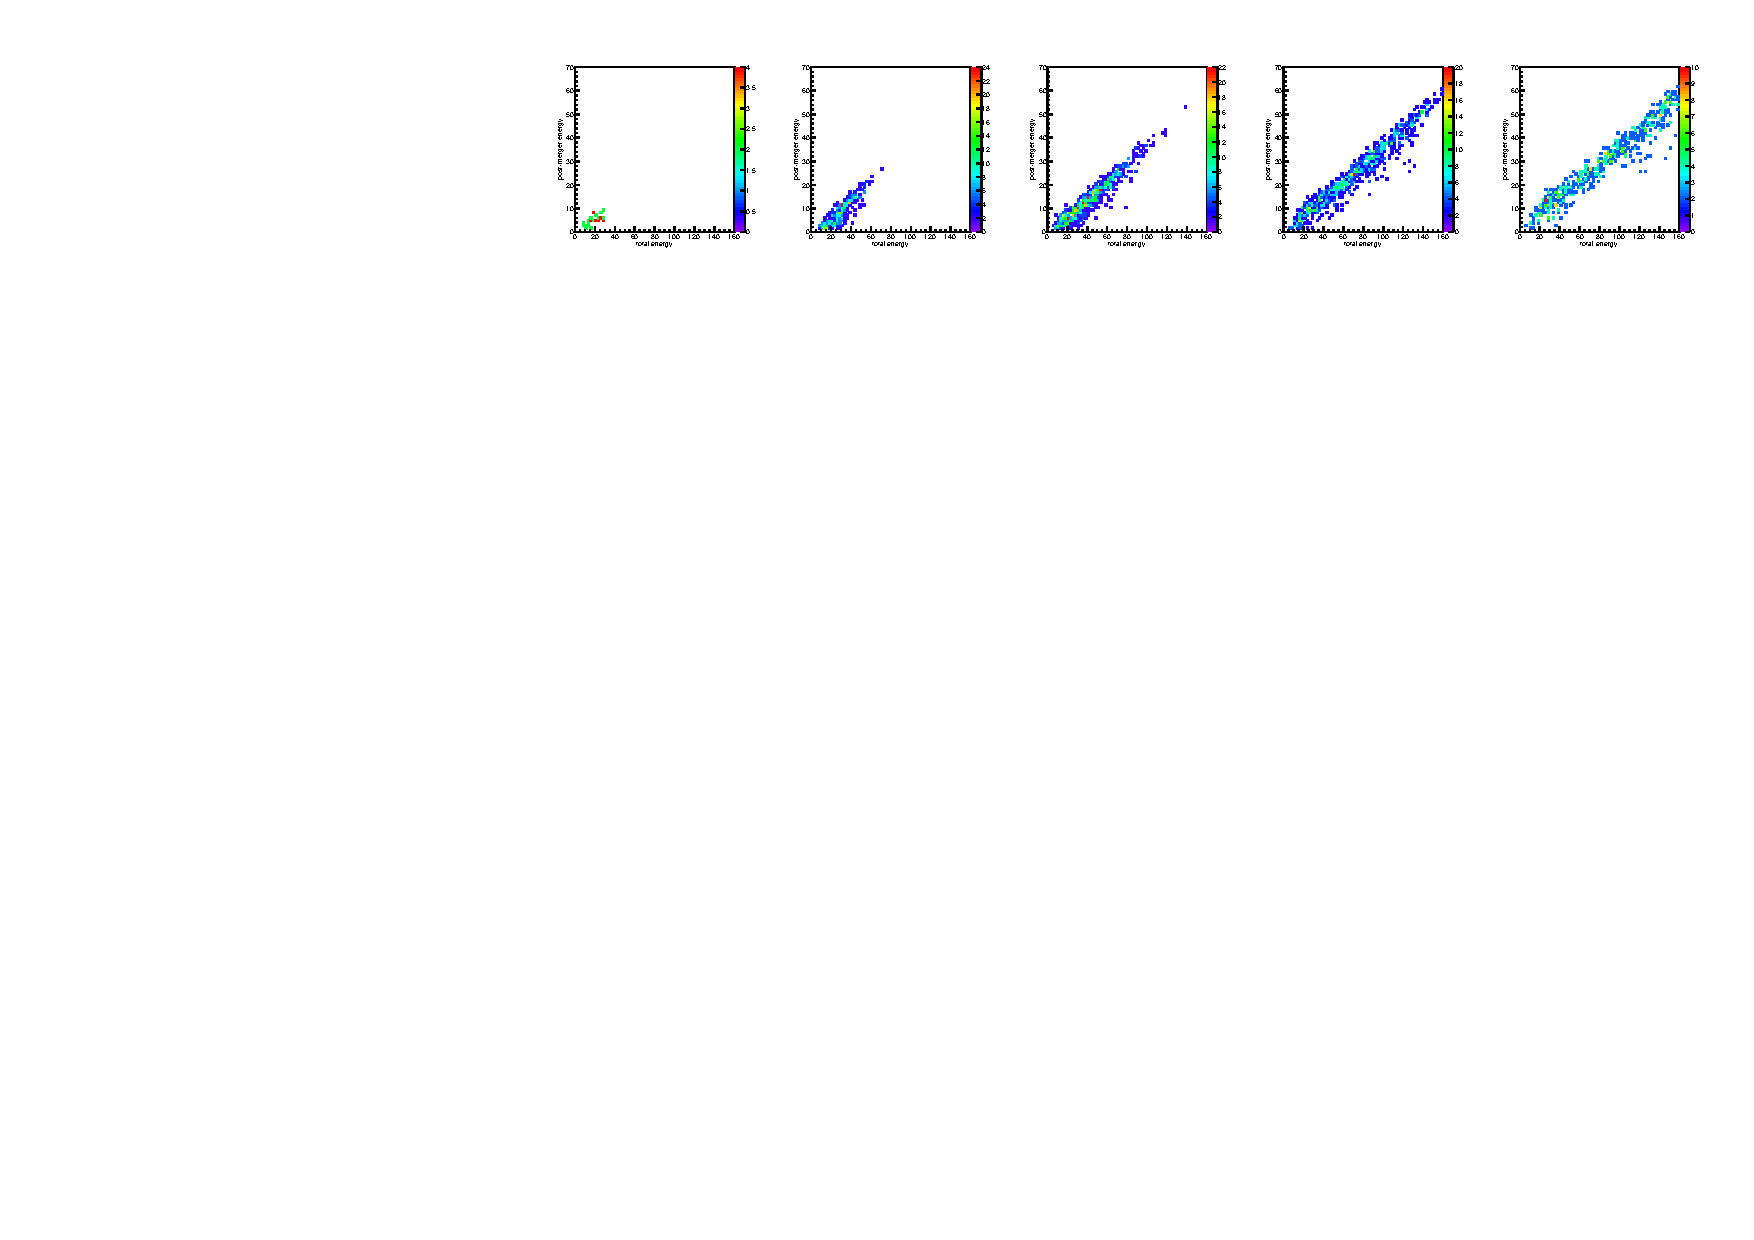
\includegraphics[width=1.\textwidth]{figures/Capitolo_3/report/EnergyDistributionFactorDetector3SHT2_0spin11.pdf}}\\
	\vspace{-13pt}
	\subfloat[][\emph{SHT2\_2}]
	{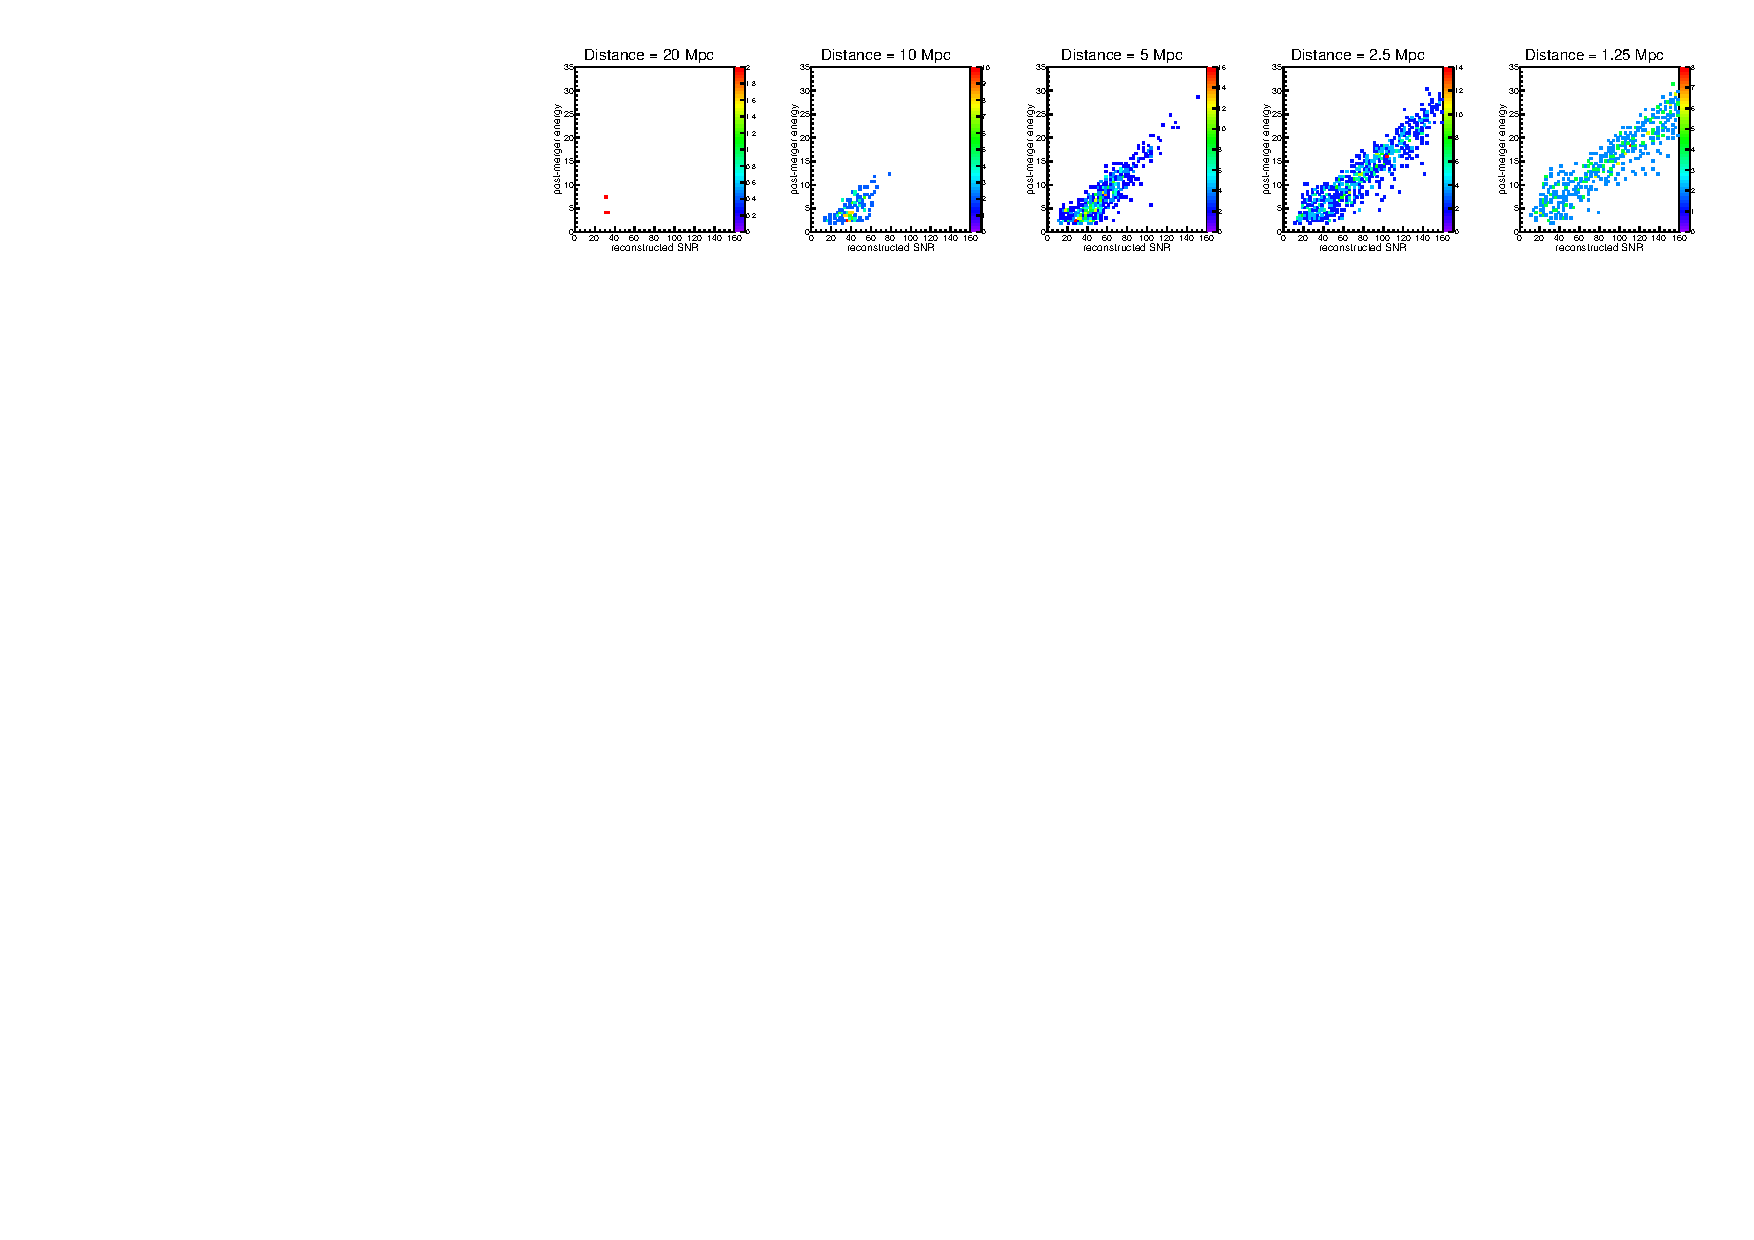
\includegraphics[width=1.\textwidth]{figures/Capitolo_3/report/EnergyDistributionFactorDetector3SHT2_2spin11.pdf}}\\
	\vspace{-13pt}
	\subfloat[][\emph{APR4}]
	{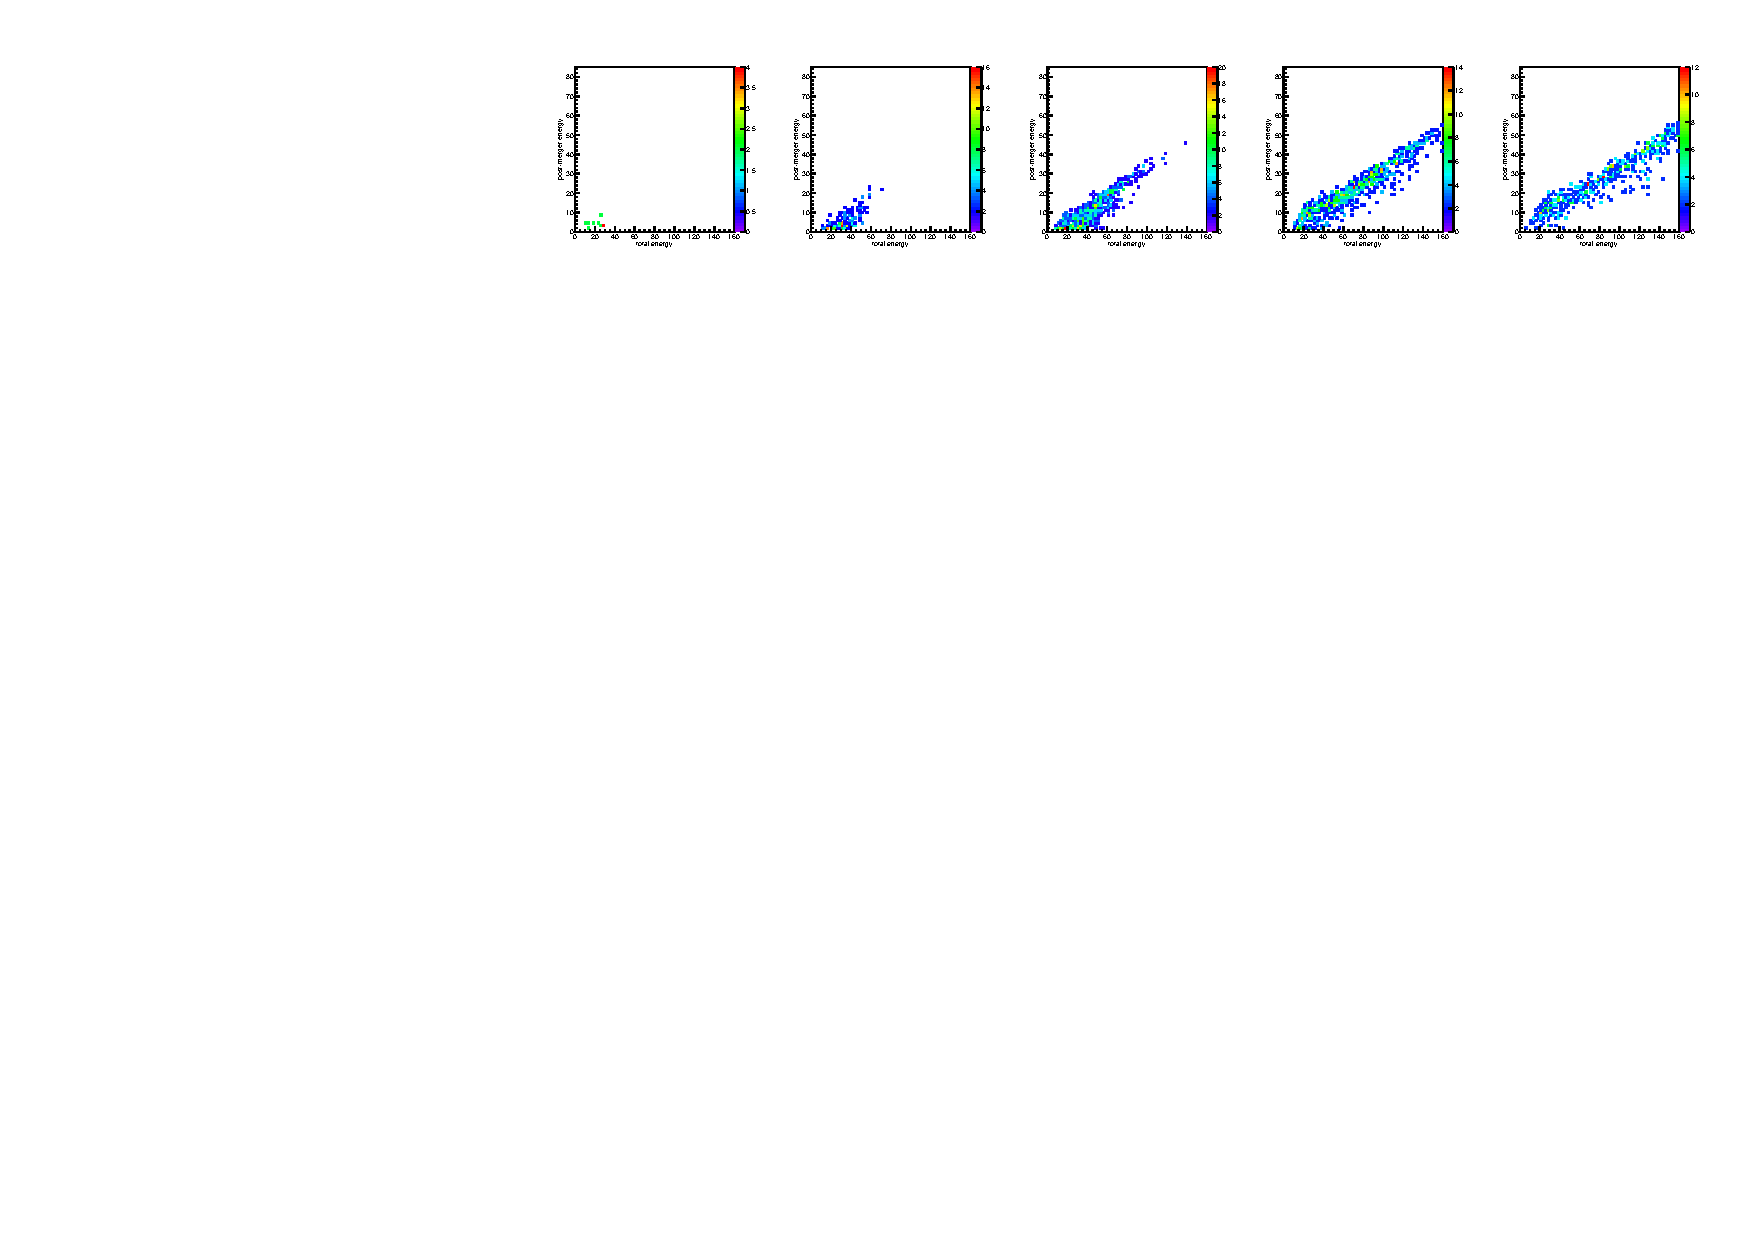
\includegraphics[width=1.\textwidth]{figures/Capitolo_3/report/EnergyDistributionFactorDetector3APR4_q091.pdf}}\vspace{-8pt}
	\caption{Distribuzione delle energie della post coalescenza in funzione dell'energia totale ricostruita in Virgo}
	\label{fig:energy_pm_colz}
\end{figure}\\
Con una analisi analoga a quella fatta per l'overlap, quindi con la divisione degli eventi in bin di SNR, si costruisce la distribuzione delle energie della post-coalescenza, riportata in Figura \ref{fig:energy_pm_Distrib}. Si nota che il segnale ricostruito da Virgo è sistematicamente più energetico del segnale ricostruito da LIGO, grazie alla maggior sensibilità del primo ad alte frequenza. Si sottilinea che comunque la sensibilità di Virgo è sovrastimata per l'assenza della caratterizzazione di risonanze e altri fenomeni che ne comprometterebbero la sensibilità.
\begin{figure}[hbt!]
	\vspace{-20pt}
	\centering
	\subfloat[][\emph{SHT2\_0}]
	{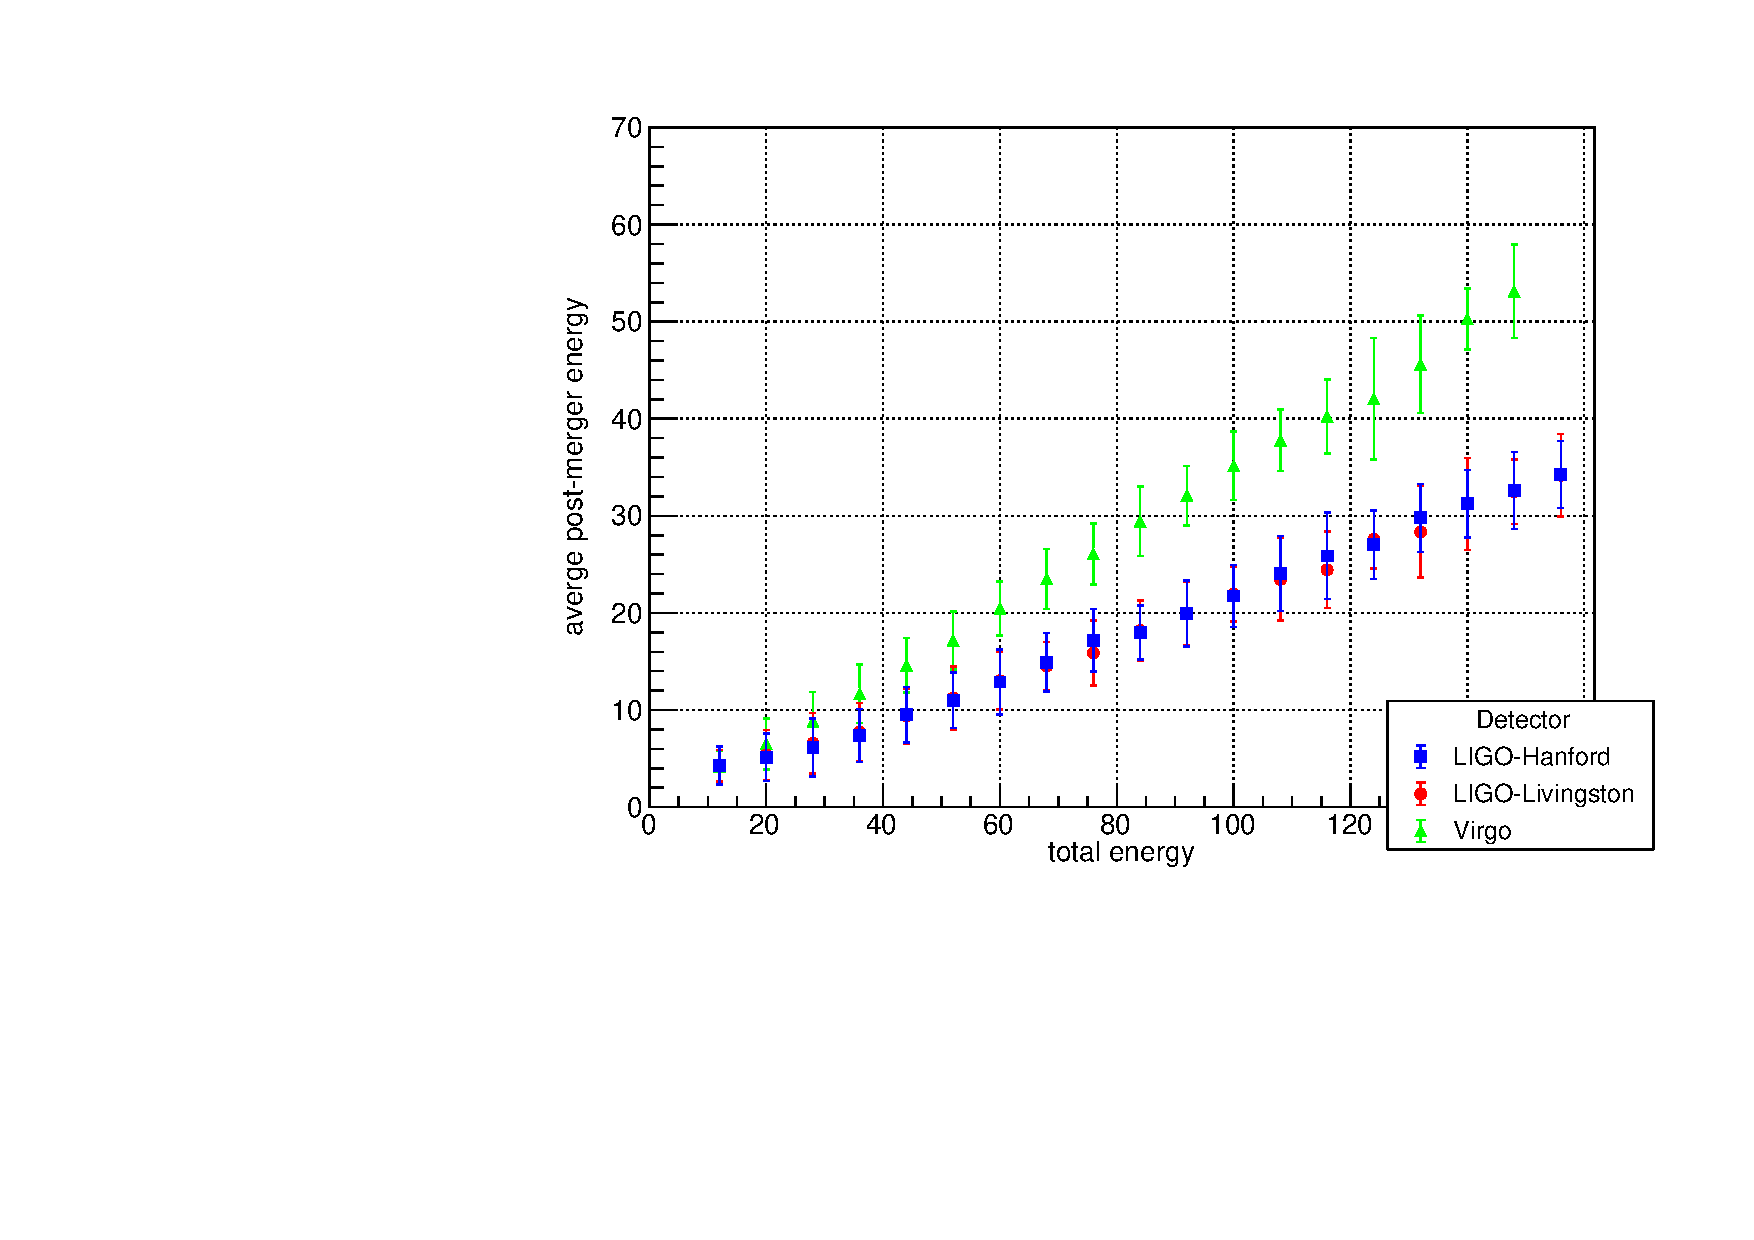
\includegraphics[width=.33333333333\textwidth]{figures/Capitolo_3/report/energy_pm_Colors_GrapgSHT2_0spin11.pdf}}
	\subfloat[][\emph{SHT2\_2}]
	{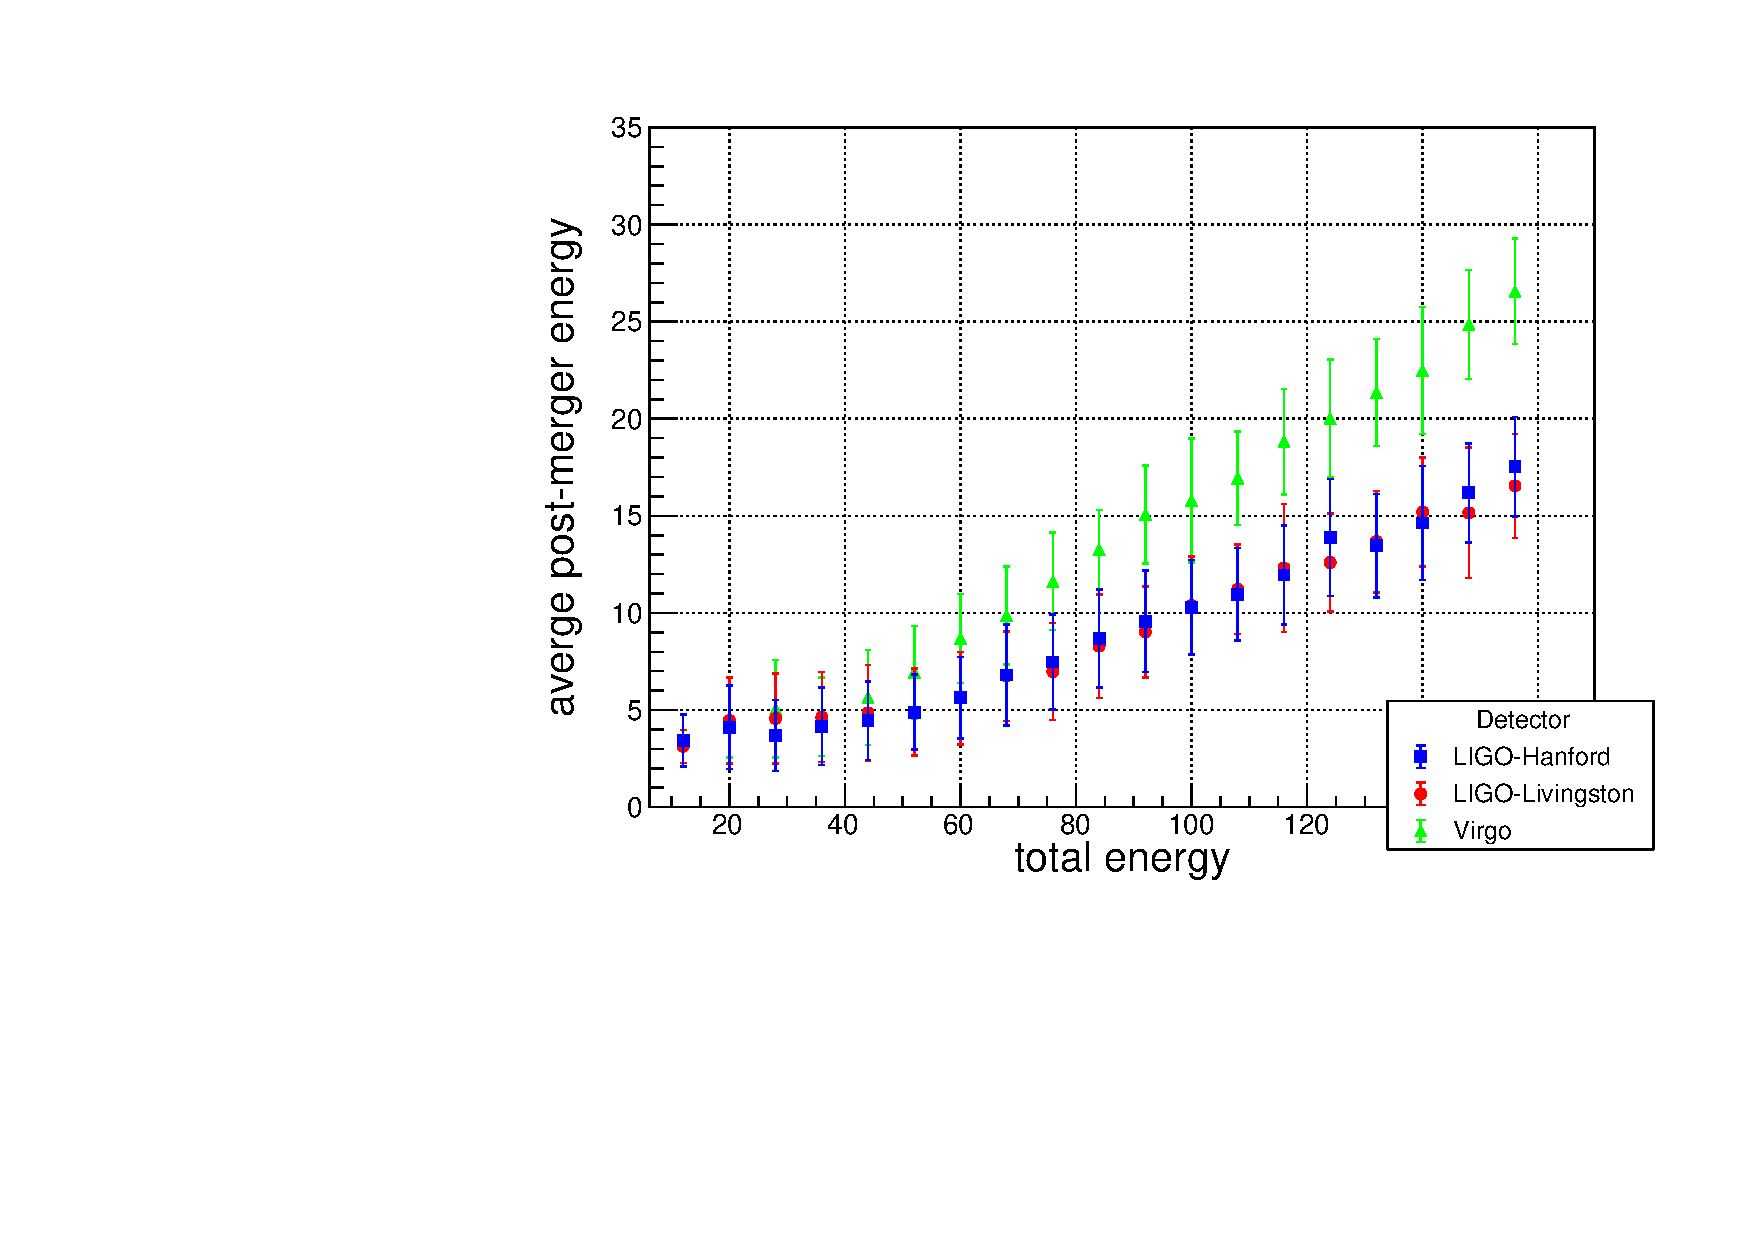
\includegraphics[width=.33333333333\textwidth]{figures/Capitolo_3/report/energy_pm_Colors_GrapgSHT2_2spin11.pdf}}
	\subfloat[][\emph{APR4}]
	{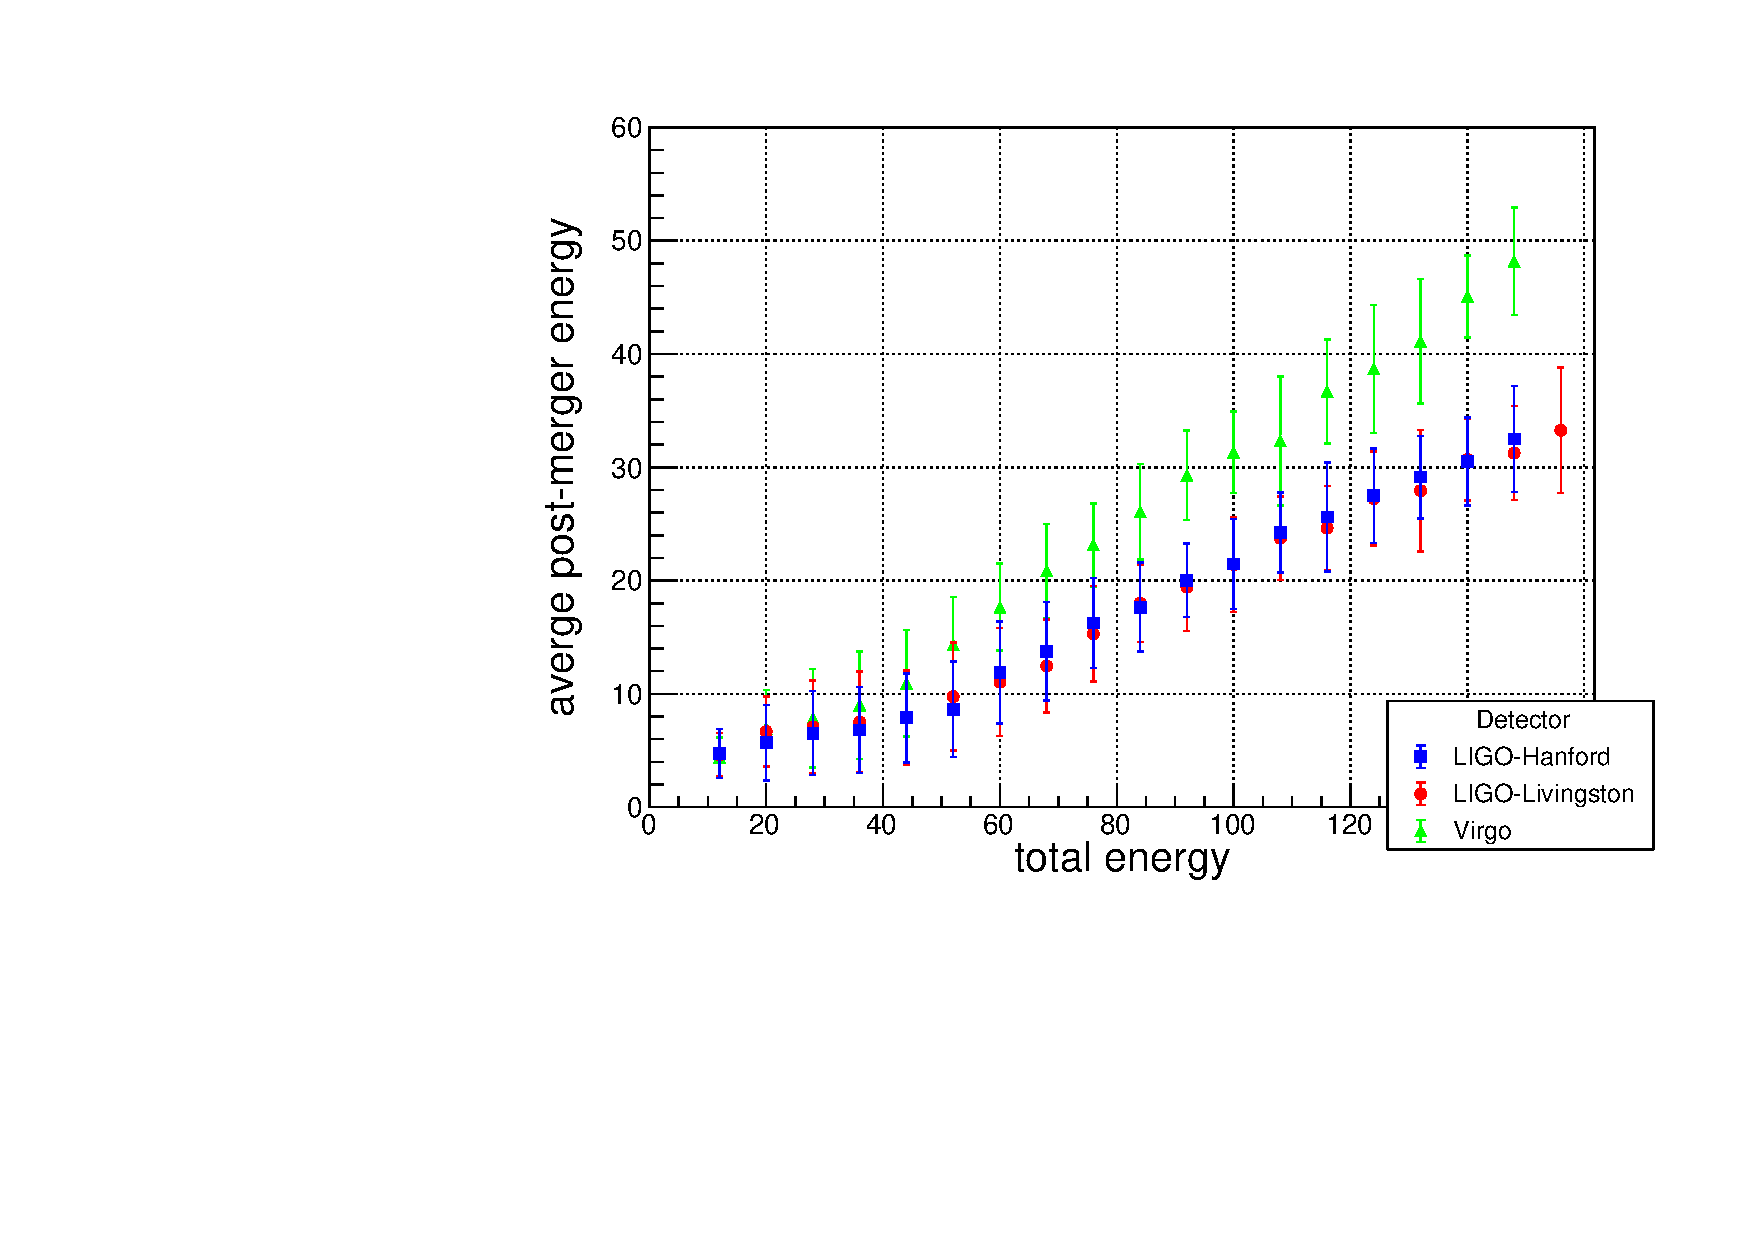
\includegraphics[width=.33333333333\textwidth]{figures/Capitolo_3/report/energy_pm_Colors_GrapgAPR4_q091.pdf}}
	\caption{Distribuzione delle energie della post coalescenza in funzione dell'energia totale ricostruita nei tre rivelatori}
	\label{fig:energy_pm_Distrib}
\end{figure}

Si riporta poi la frequenza alla quale vengono ricostruiti i segnali di post-coalescenza e le distribuzioni dividendo per bin di SNR a larghezza fissata, in Figura \ref{fig:frequency_pm_Distrib}. Quello che si osserva è che la frequenza ricostruita risulta generalmente superiore per Virgo, rispetto ai rivelatori LIGO, per motivi analoghi a quello che porta segnali più energetici per il primo. È interessante anche osservare l'andamento che non è strettamente crescente in funzione dell'energia ricostruita, ma parte da frequenze più alte e dopo un minimo risale: questa peculiarità è spiegata dalla distribuzione dell'energia nella post-coalesenza, che risulta avere un picco corrispondente anche al picco di frequenza. Essendo quindi il picco più energetico, sarà la parte che verrà ricostruita prima, e quindi eventi meno energetici, in cui si ricostruisce la post-coalescenza, faranno riferimento al solo picco. Superata questa fase, la ricostruzione avviene come atteso.\\
In particolare, in Figura \ref{fig:frequency_pm_colz}, è riportata la distribuzione delle frequenze pesate tra i rivelatori: per ogni evento viene prodotta una media pesata tra le frequenze ricostruite in ogni interferometro, il peso è in particolare definito dall'energia ricostruita per la post-coalescenza. L'SNR ricostruito riportato è quindi, al contrario di come è riportato negli altri grafici, l'SNR totale dell'evento, ottenuto come somma in quadratura degli SNR dei singoli interferometri.\\
Si osserva, come atteso, che le frequenze ricostruite, essendo frequenze pesate, risultano sottostimate poiché nella ricostruzione viene considerata la parte finale dello spiraleggiamento, a frequenze evidentemente inferiori. Questa sottostima è particolarmente evidente nella EOS APR4, che dovrebbe avere una frequenza massima a 3.30kHz (Tab. \ref{tab:EOS}), e la frequenza pesata ottenuta è sempre al di sotto dei 3kHz.
\begin{figure}[hbt!]
	\vspace{-15pt}
	\centering
	\subfloat[][\emph{SHT2\_0}]
	{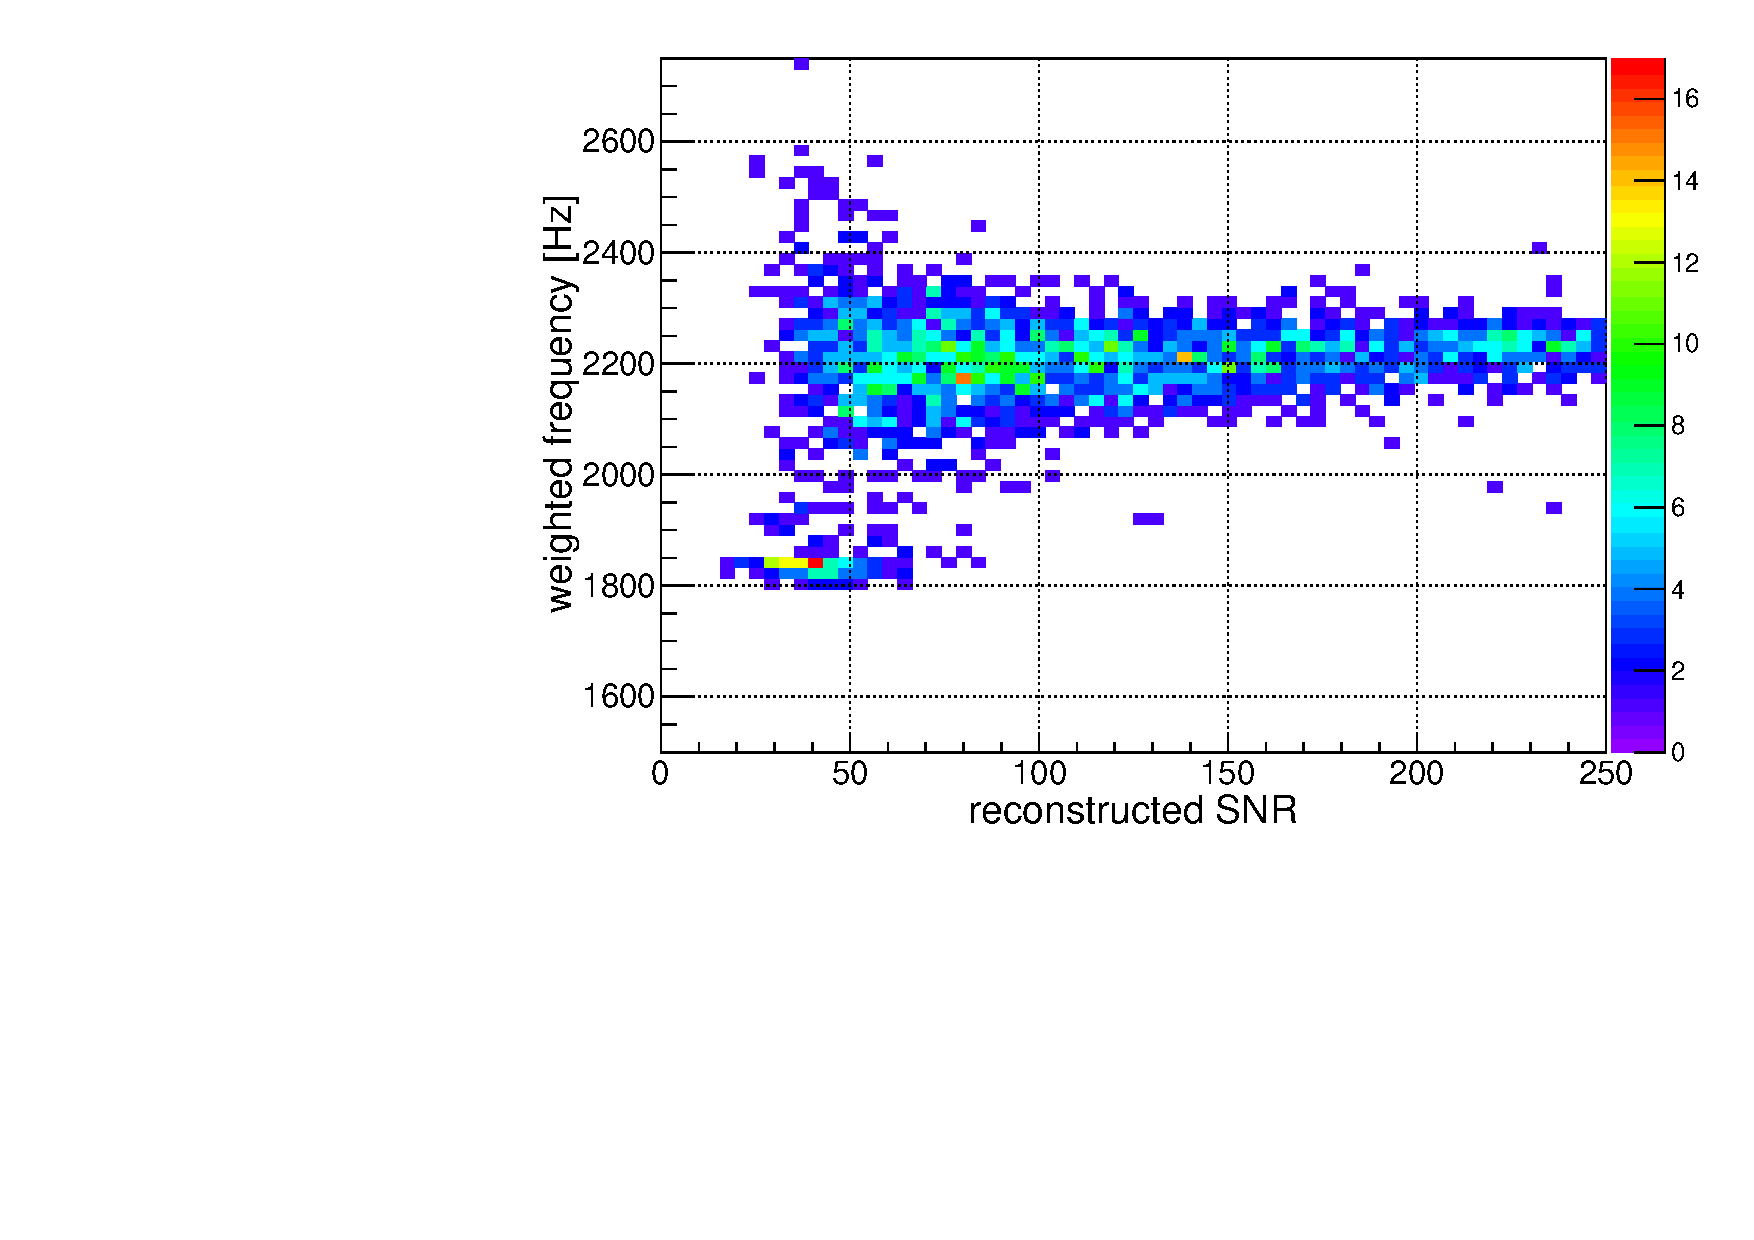
\includegraphics[width=.333333333333333333\textwidth]{figures/Capitolo_3/report/Freq_PM_DistributionDetector3SHT2_0spin10.pdf}}
	\subfloat[][\emph{SHT2\_2}]
	{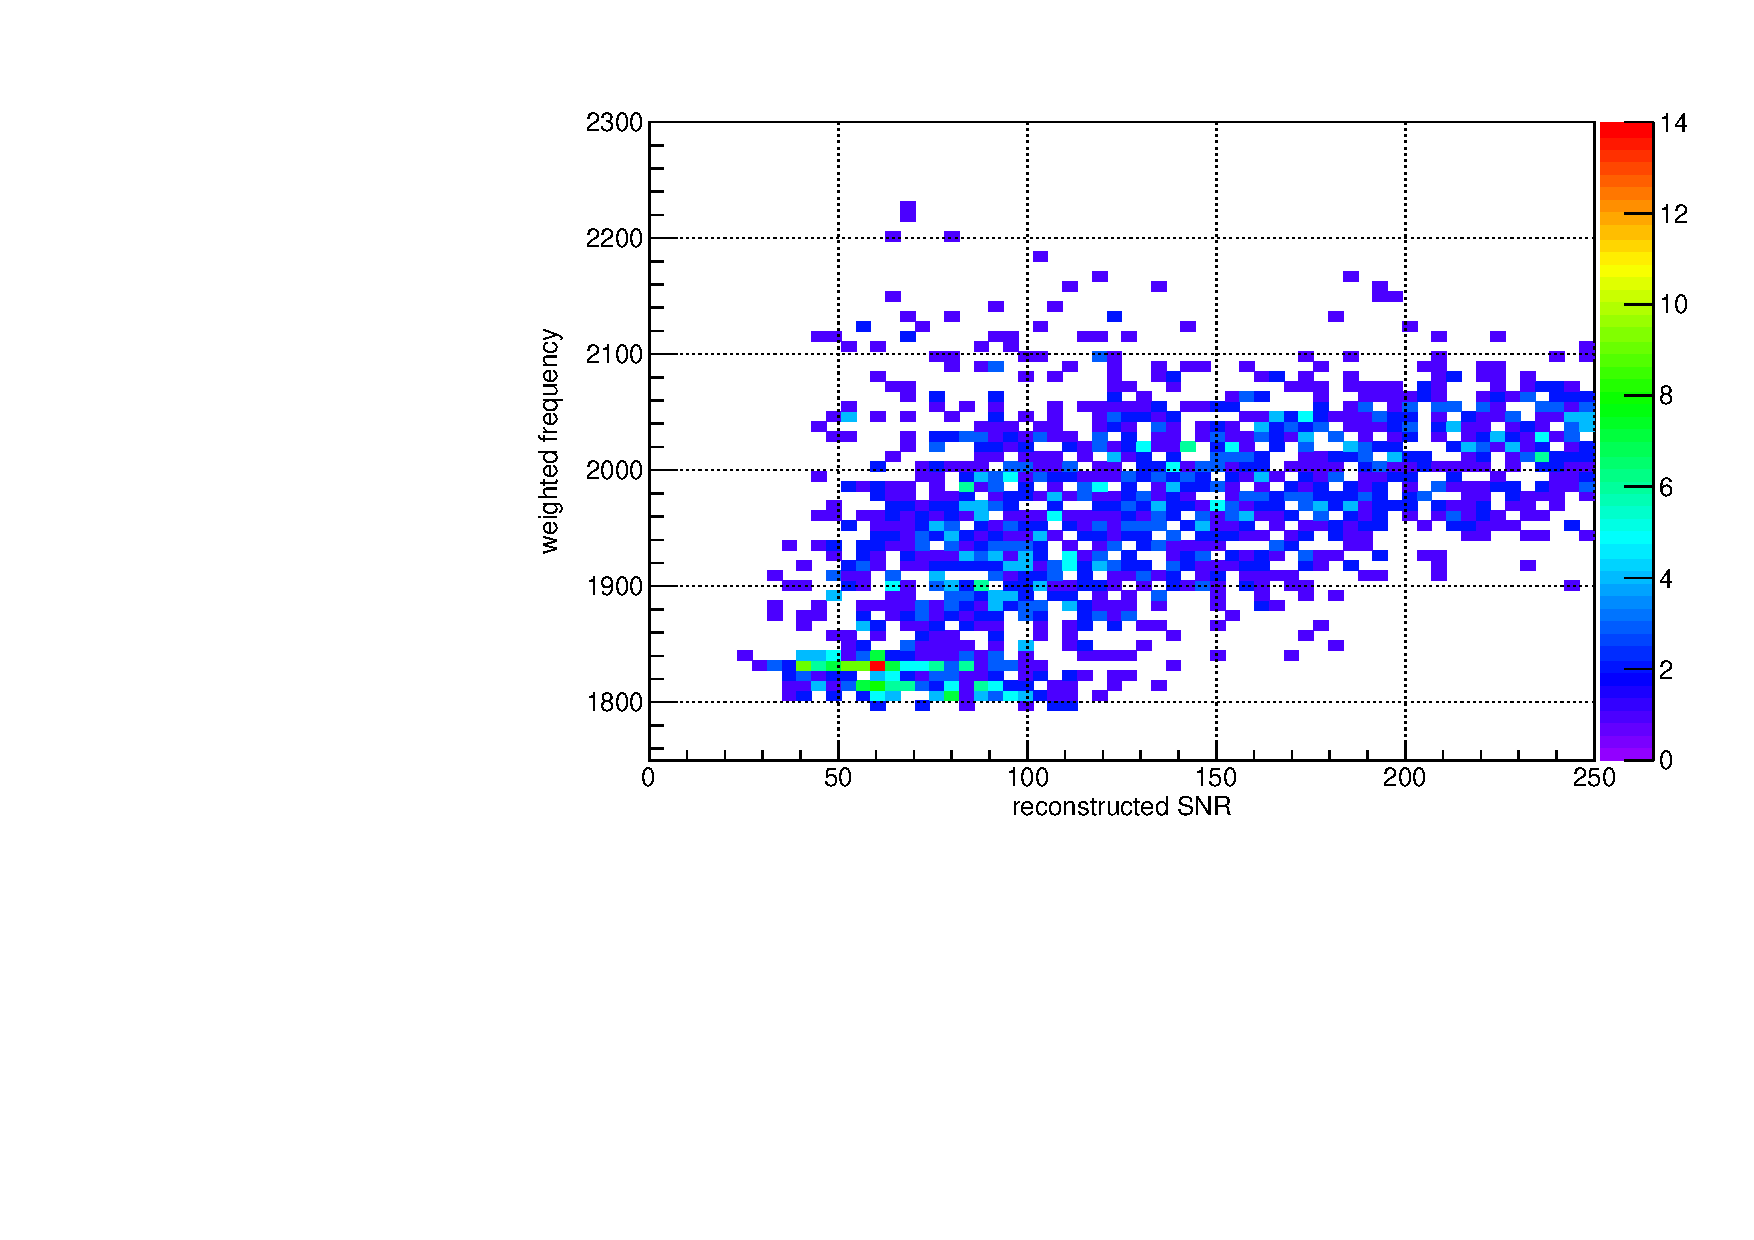
\includegraphics[width=.333333333333333333\textwidth]{figures/Capitolo_3/report/Freq_PM_DistributionDetector3SHT2_2spin10.pdf}}
	\subfloat[][\emph{APR4}]
	{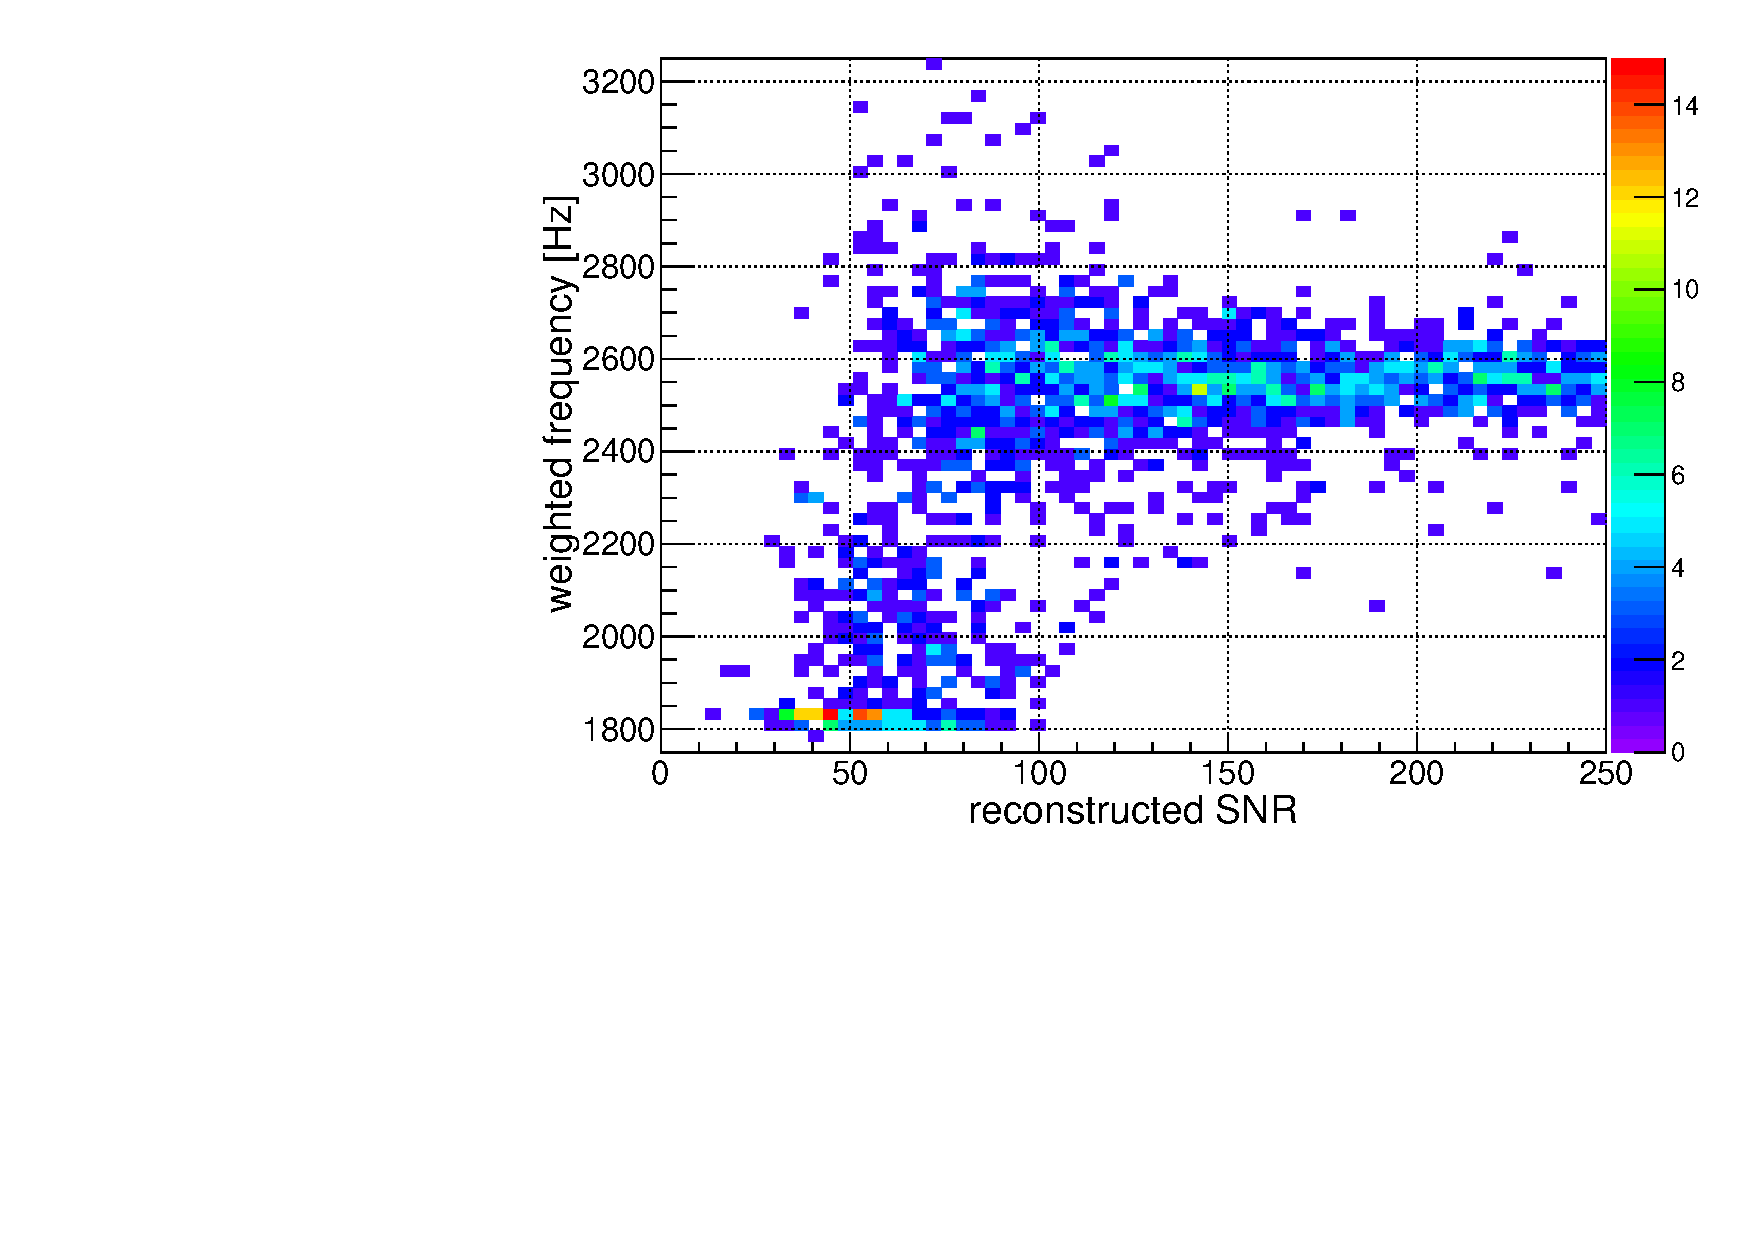
\includegraphics[width=.333333333333333333\textwidth]{figures/Capitolo_3/report/Freq_PM_DistributionDetector3APR4_q090.pdf}}
	\caption{Distribuzione delle medie pesate con l'energia della post-coalescenza della frequenza ricostruita da ogni rivelatore in funzione dell'energia totale dell'evento}
	\label{fig:frequency_pm_colz}
\end{figure}
\begin{figure}[hbt!]
	\vspace{-15pt}
	\centering
	\subfloat[][\emph{SHT2\_0}]
	{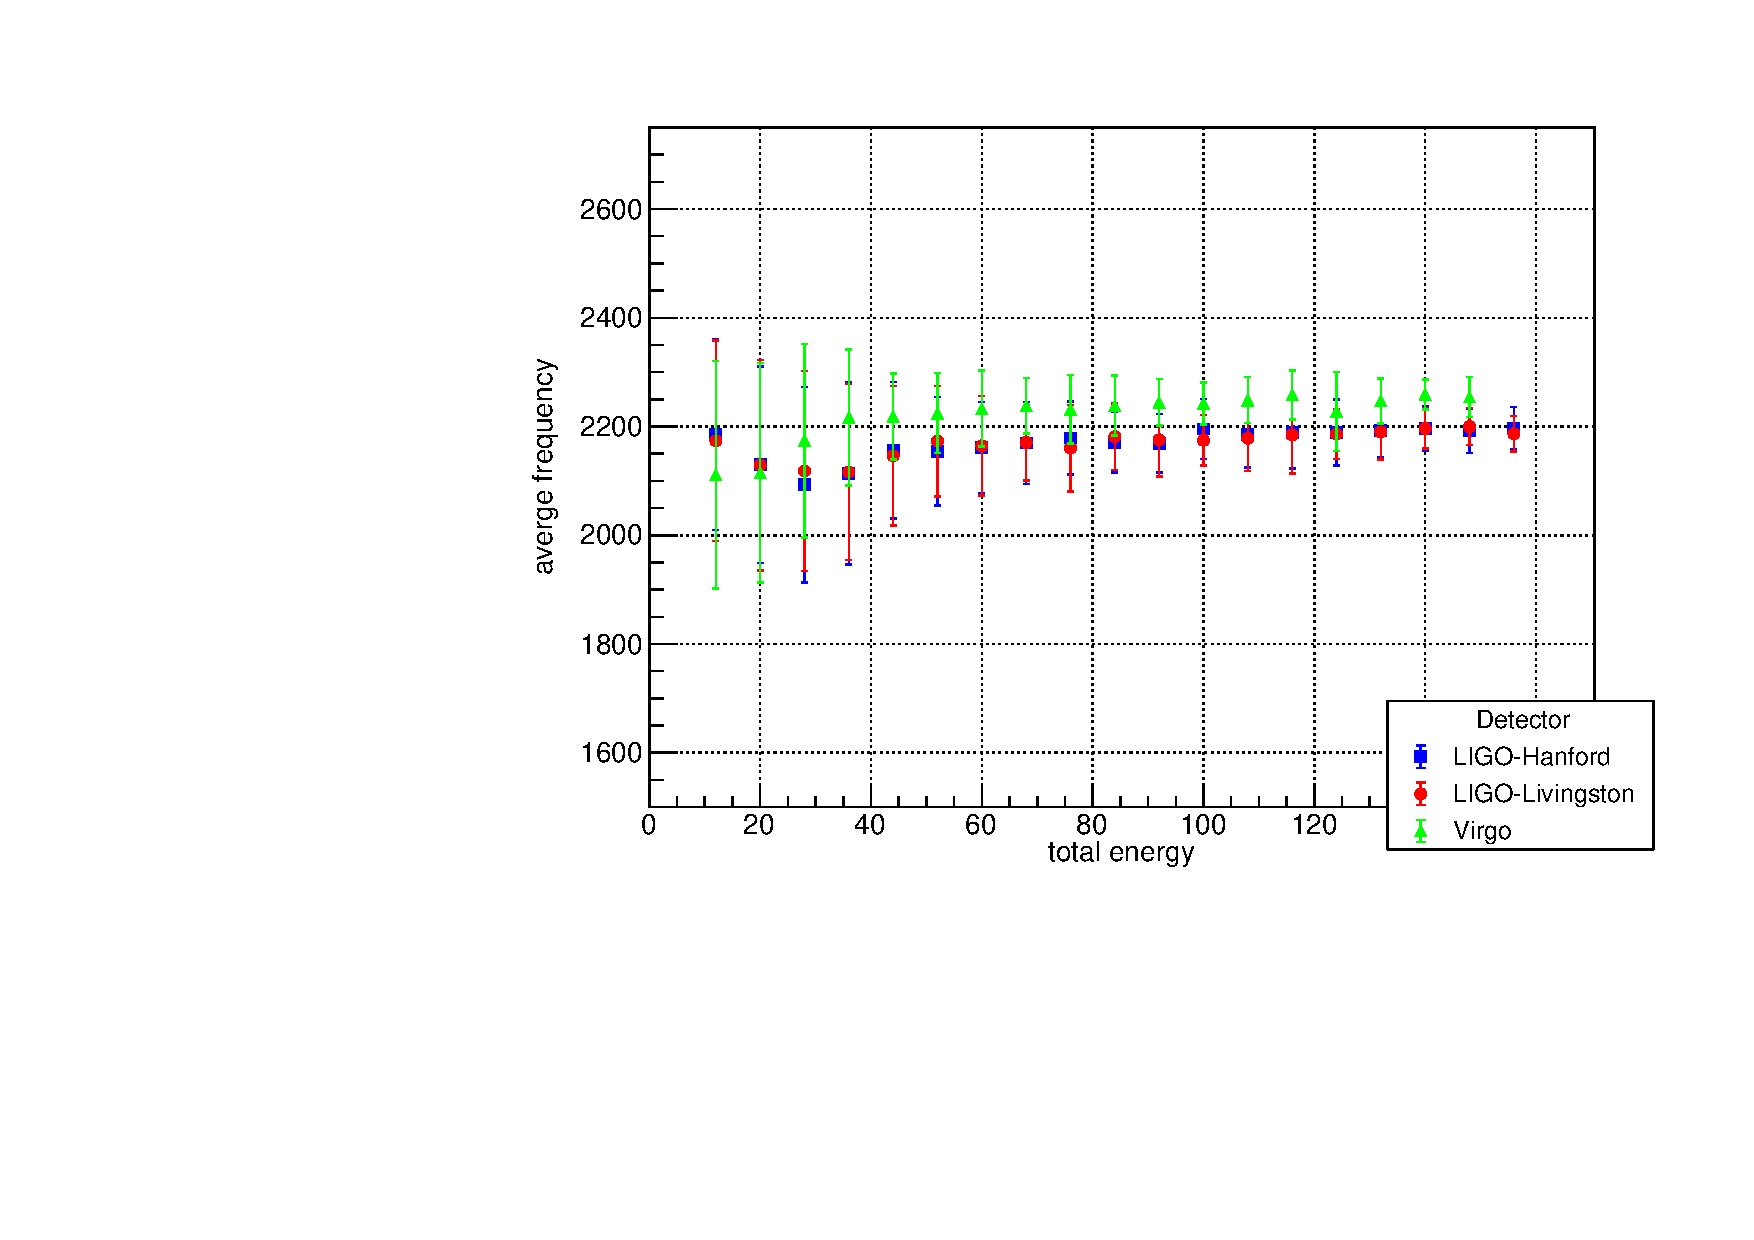
\includegraphics[width=.33333333333\textwidth]{figures/Capitolo_3/report/frequencies_Colors_GrapgSHT2_0spin11.pdf}}
	\subfloat[][\emph{SHT2\_2}]
	{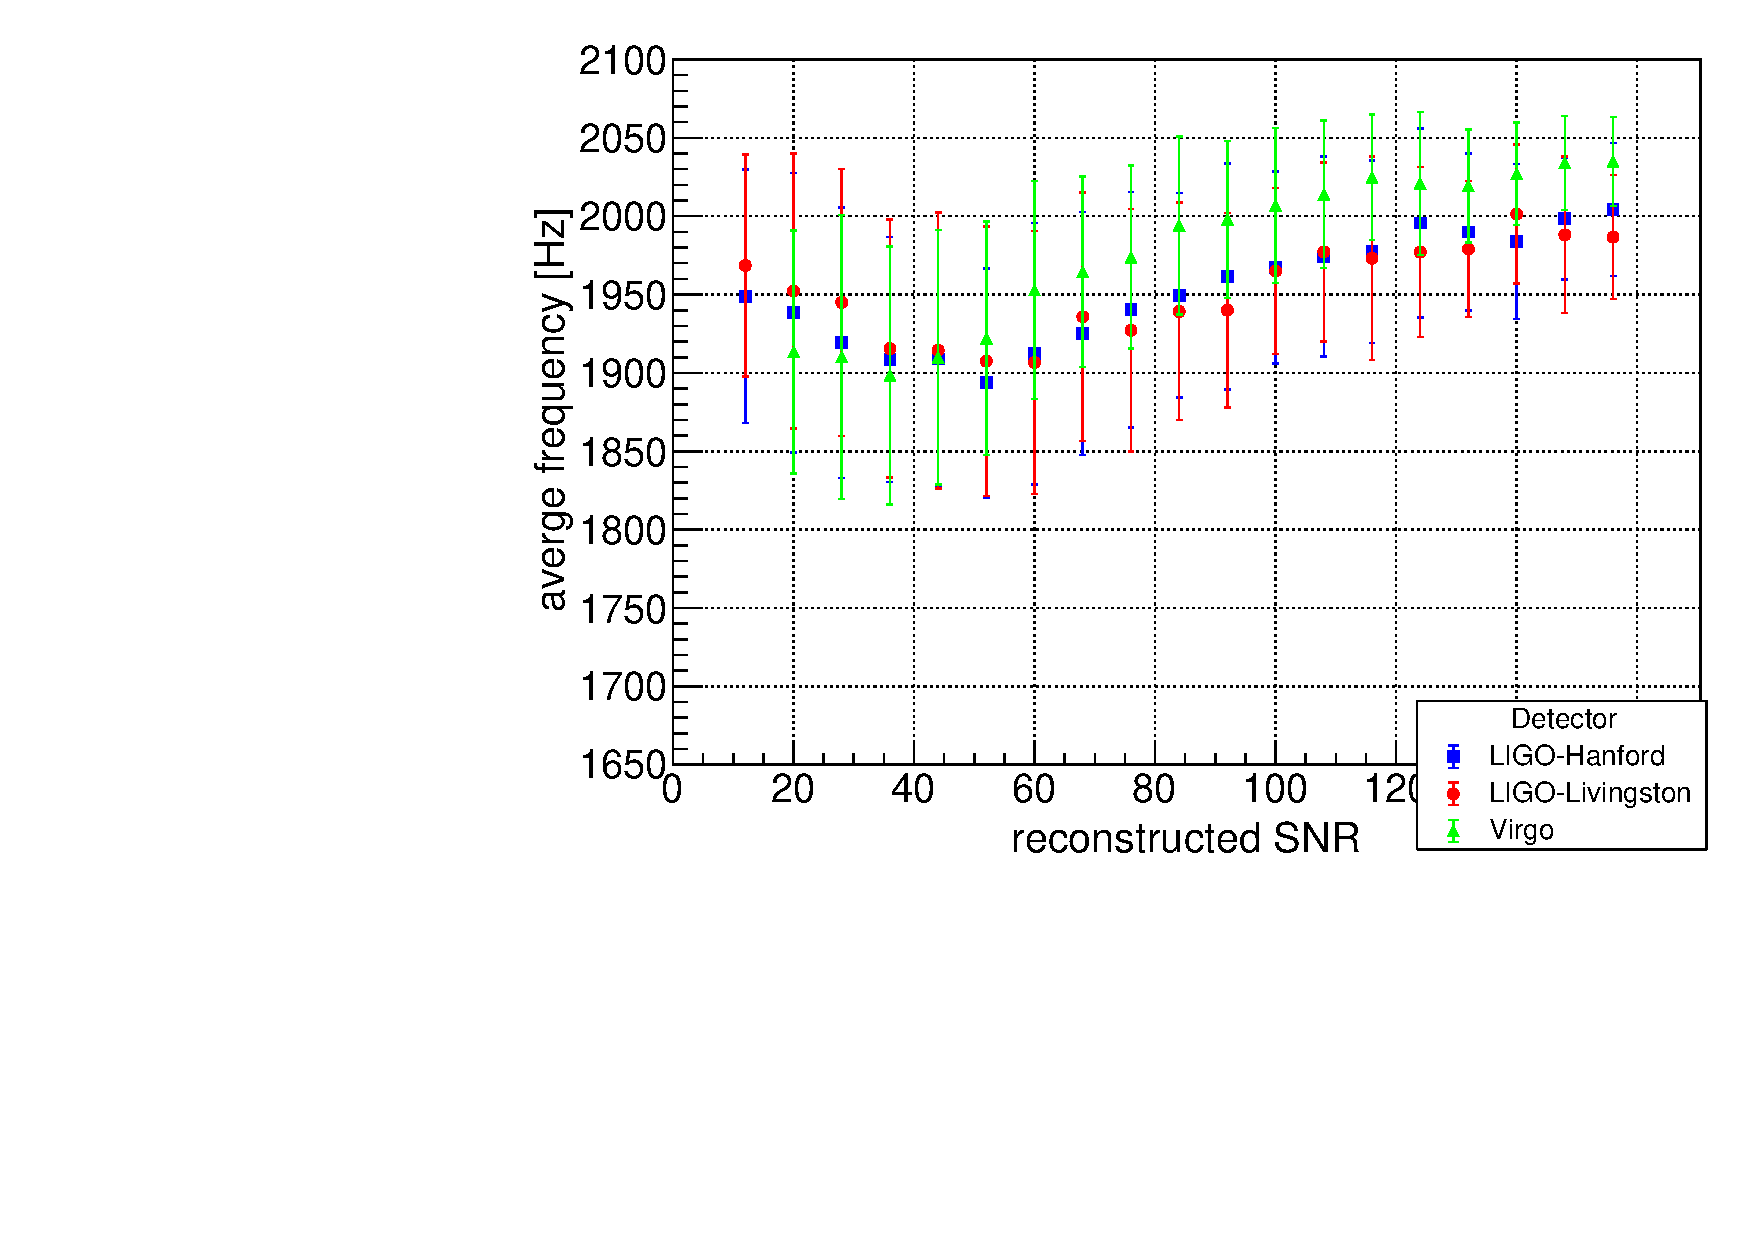
\includegraphics[width=.33333333333\textwidth]{figures/Capitolo_3/report/frequencies_Colors_GrapgSHT2_2spin11.pdf}}
	\subfloat[][\emph{APR4}]
	{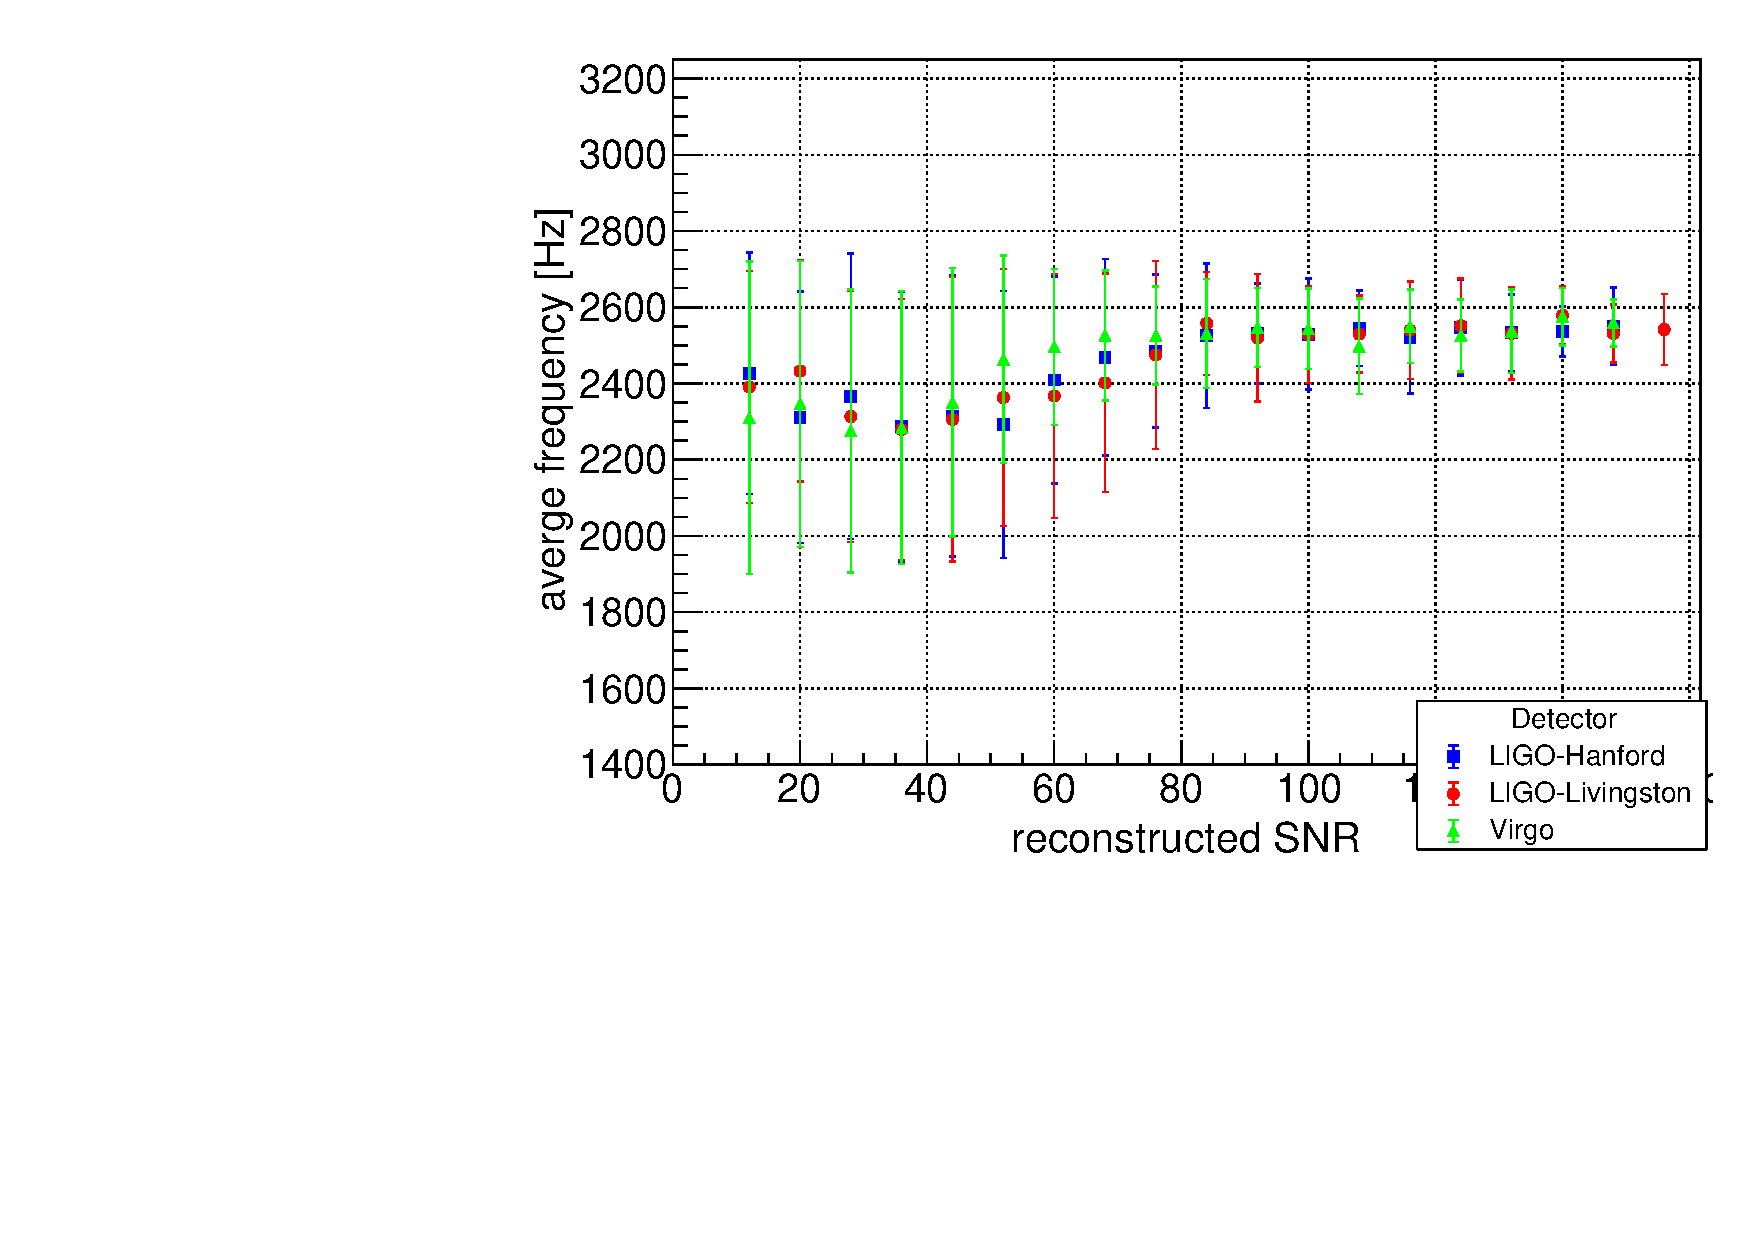
\includegraphics[width=.33333333333\textwidth]{figures/Capitolo_3/report/frequencies_Colors_GrapgAPR4_q091.pdf}}
	\caption{Distribuzione delle frequenze della post coalescenza in funzione dell'energia totale ricostruita nei tre rivelatori}
	\label{fig:frequency_pm_Distrib}
\end{figure}

Si riporta poi, in Figura \ref{fig:bandwidth_pm_Distrib}, la distribuzione della larghezza di banda dei segnali ricostruiti, ovvero la differenza tra la frequenza massima e minima rivelate. Si nota che essa ha un andamento analogo a quello della frequenza, motivo per il quale la probabilità di rivelare il segnale aumenta con l'aumentare dell'SNR.
\begin{figure}[hbt!]
	%	\vspace{-15pt}
	\centering
	\subfloat[][\emph{SHT2\_0}]
	{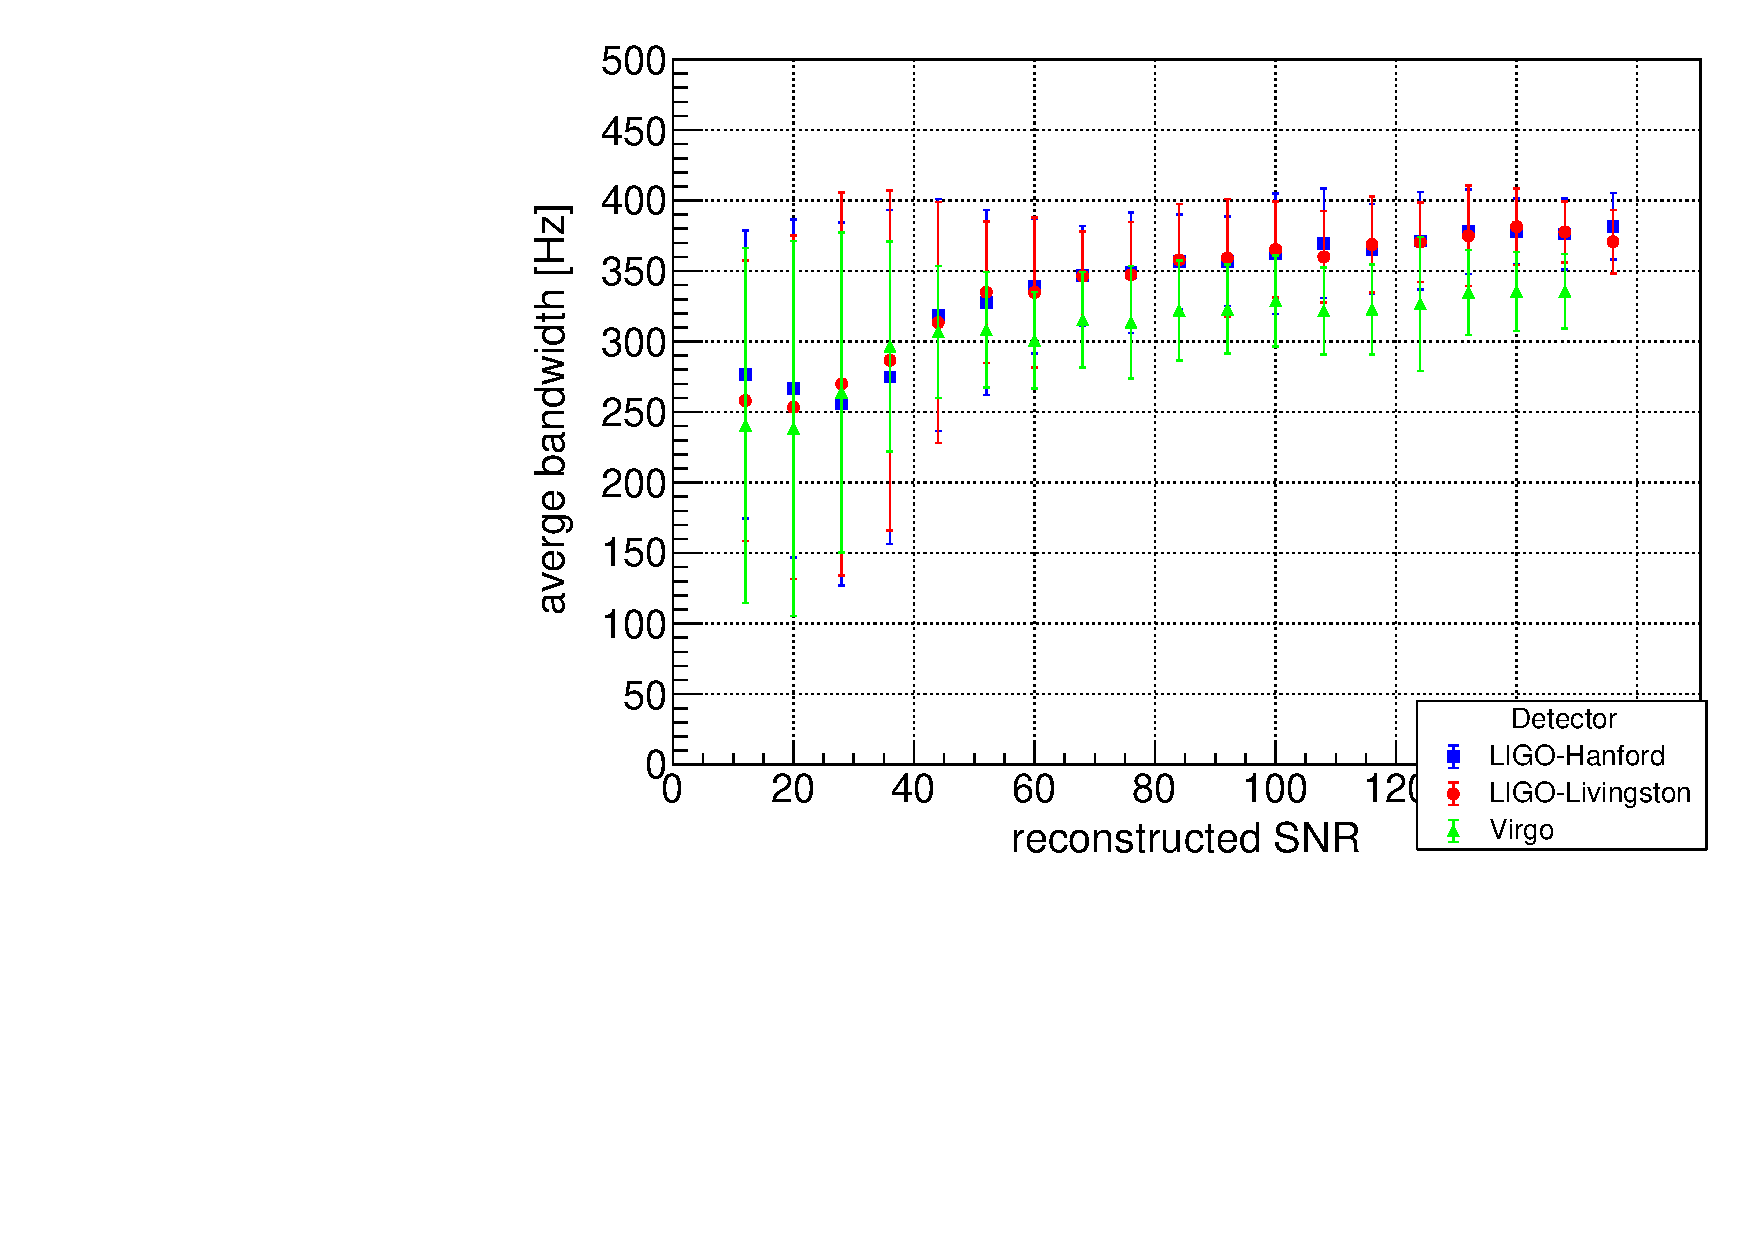
\includegraphics[width=.33333333333\textwidth]{figures/Capitolo_3/report/bandwidth_Colors_GrapgSHT2_0spin11.pdf}}
	\subfloat[][\emph{SHT2\_2}]
	{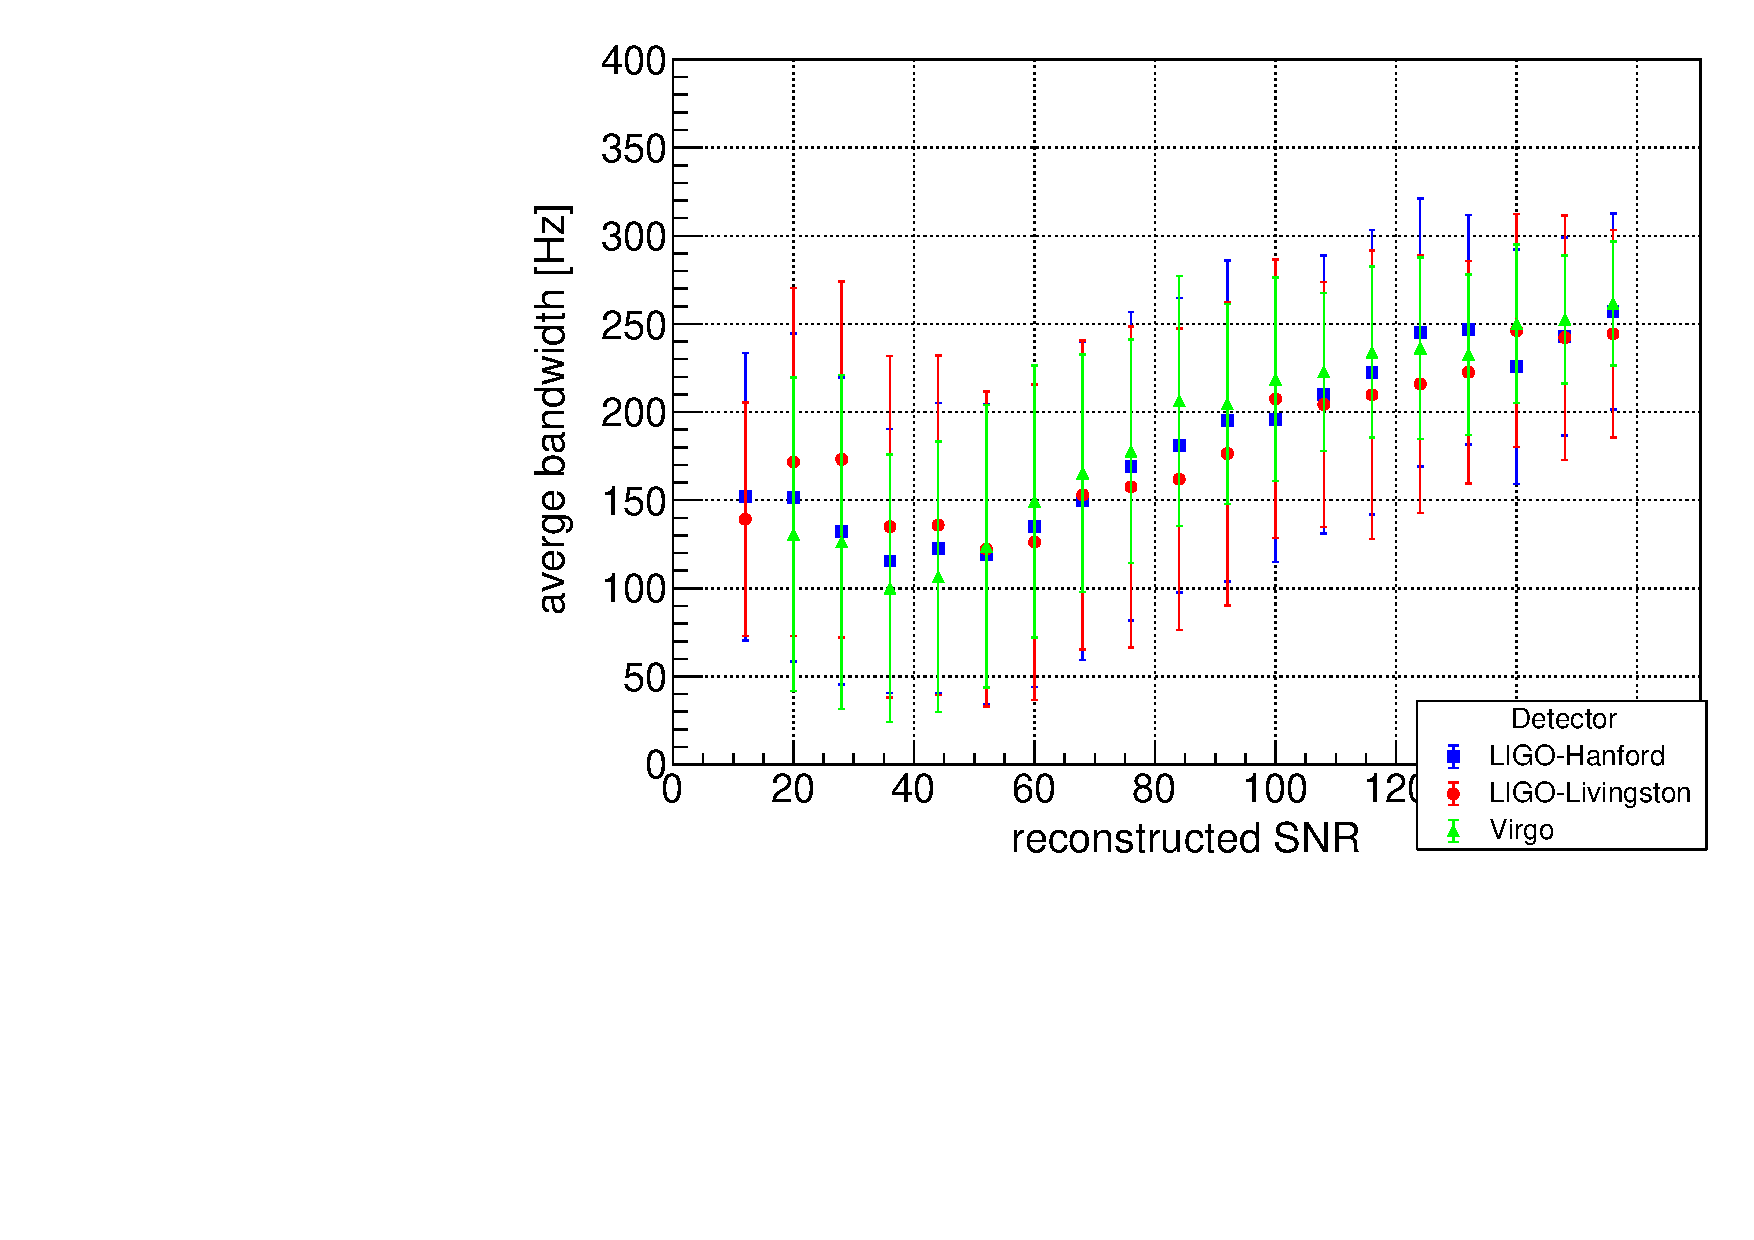
\includegraphics[width=.33333333333\textwidth]{figures/Capitolo_3/report/bandwidth_Colors_GrapgSHT2_2spin11.pdf}}
	\subfloat[][\emph{APR4}]
	{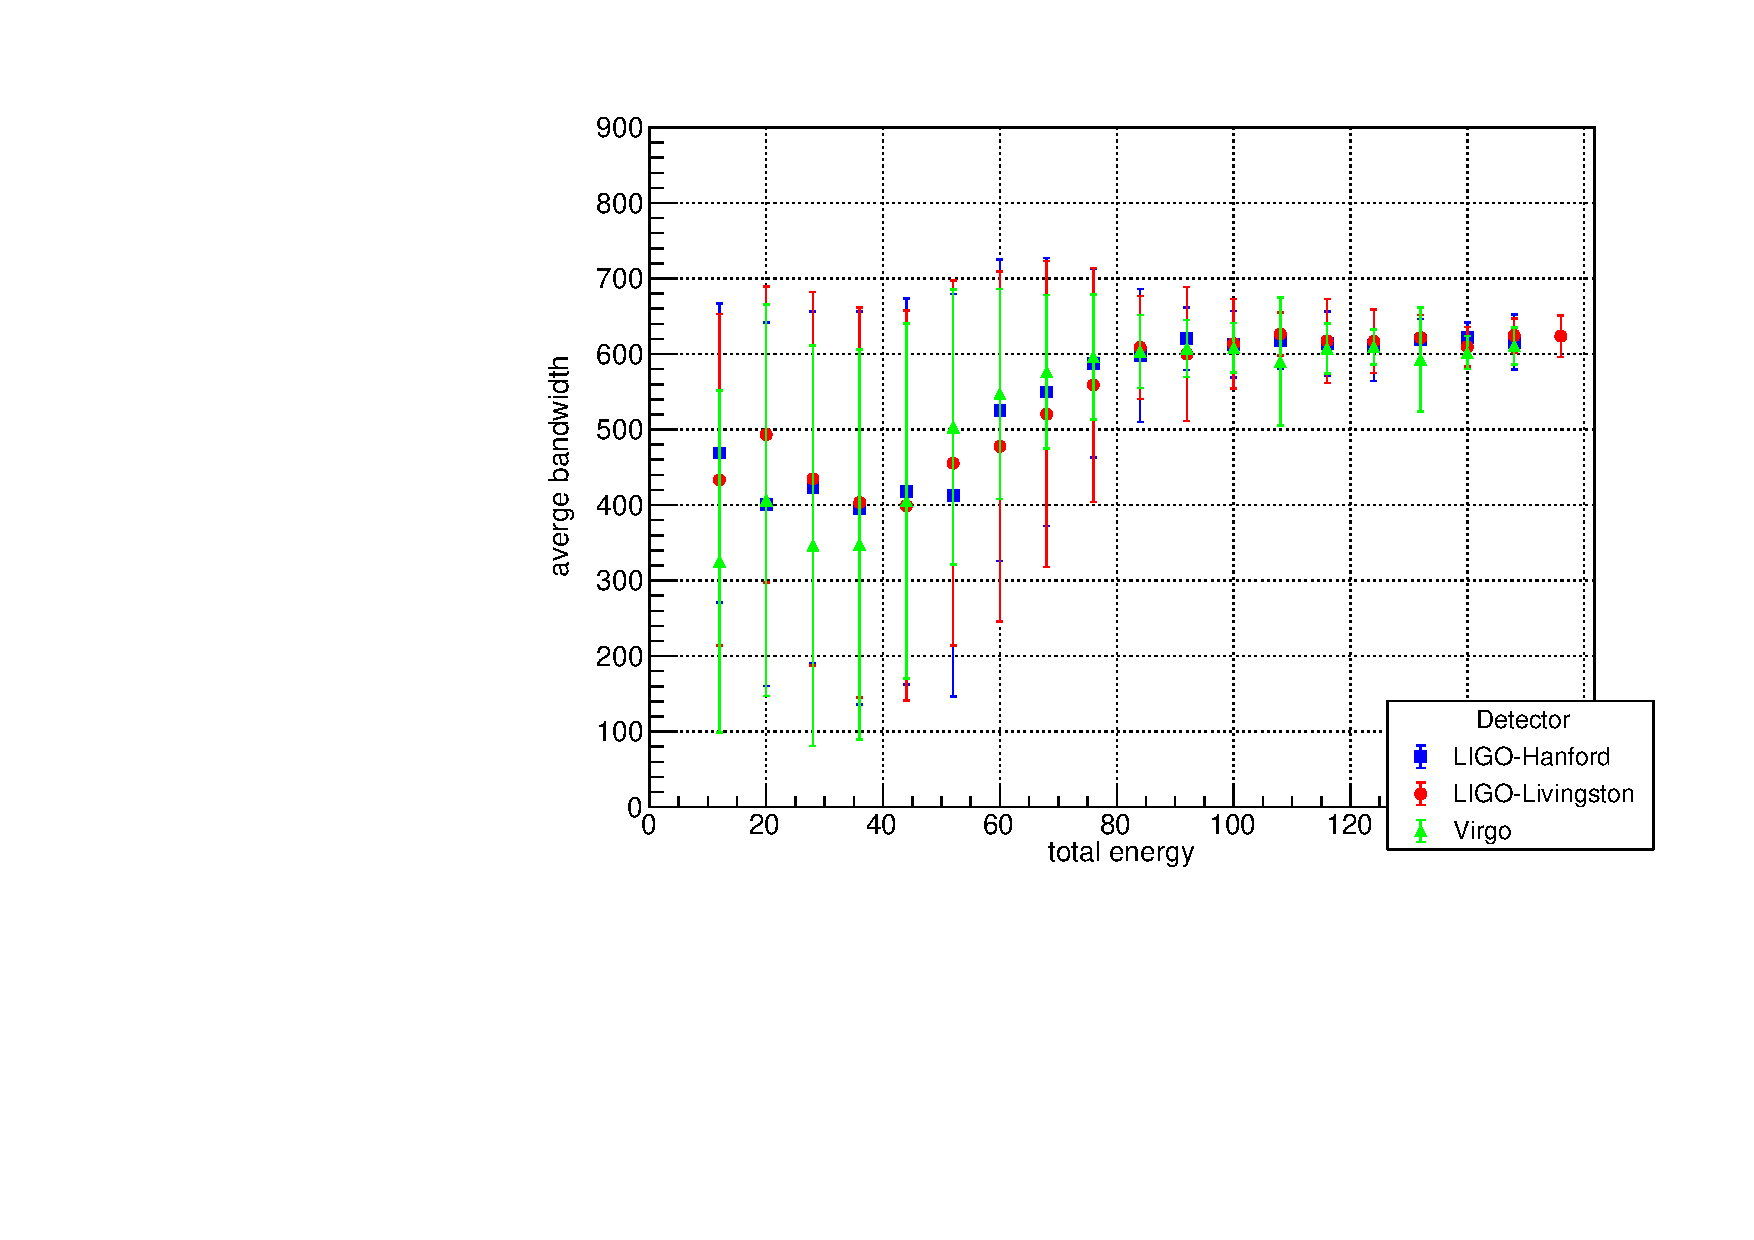
\includegraphics[width=.33333333333\textwidth]{figures/Capitolo_3/report/bandwidth_Colors_GrapgAPR4_q091.pdf}}\\
	\caption{Distribuzione delle larghezze di banda della post coalescenza in funzione dell'energia totale ricostruita nei tre rivelatori}
	\label{fig:bandwidth_pm_Distrib}
\end{figure}
%
%È interessante anche osservare la distribuzione delle energie della post-coalescenza in funzione della verosimiglianza dell'evento, in Figura \ref{fig:likelihood}.
%\begin{figure}[hbt!]
%	\vspace{-15pt}
%	\centering
%	\subfloat[][\emph{SHT2\_0}]
%	{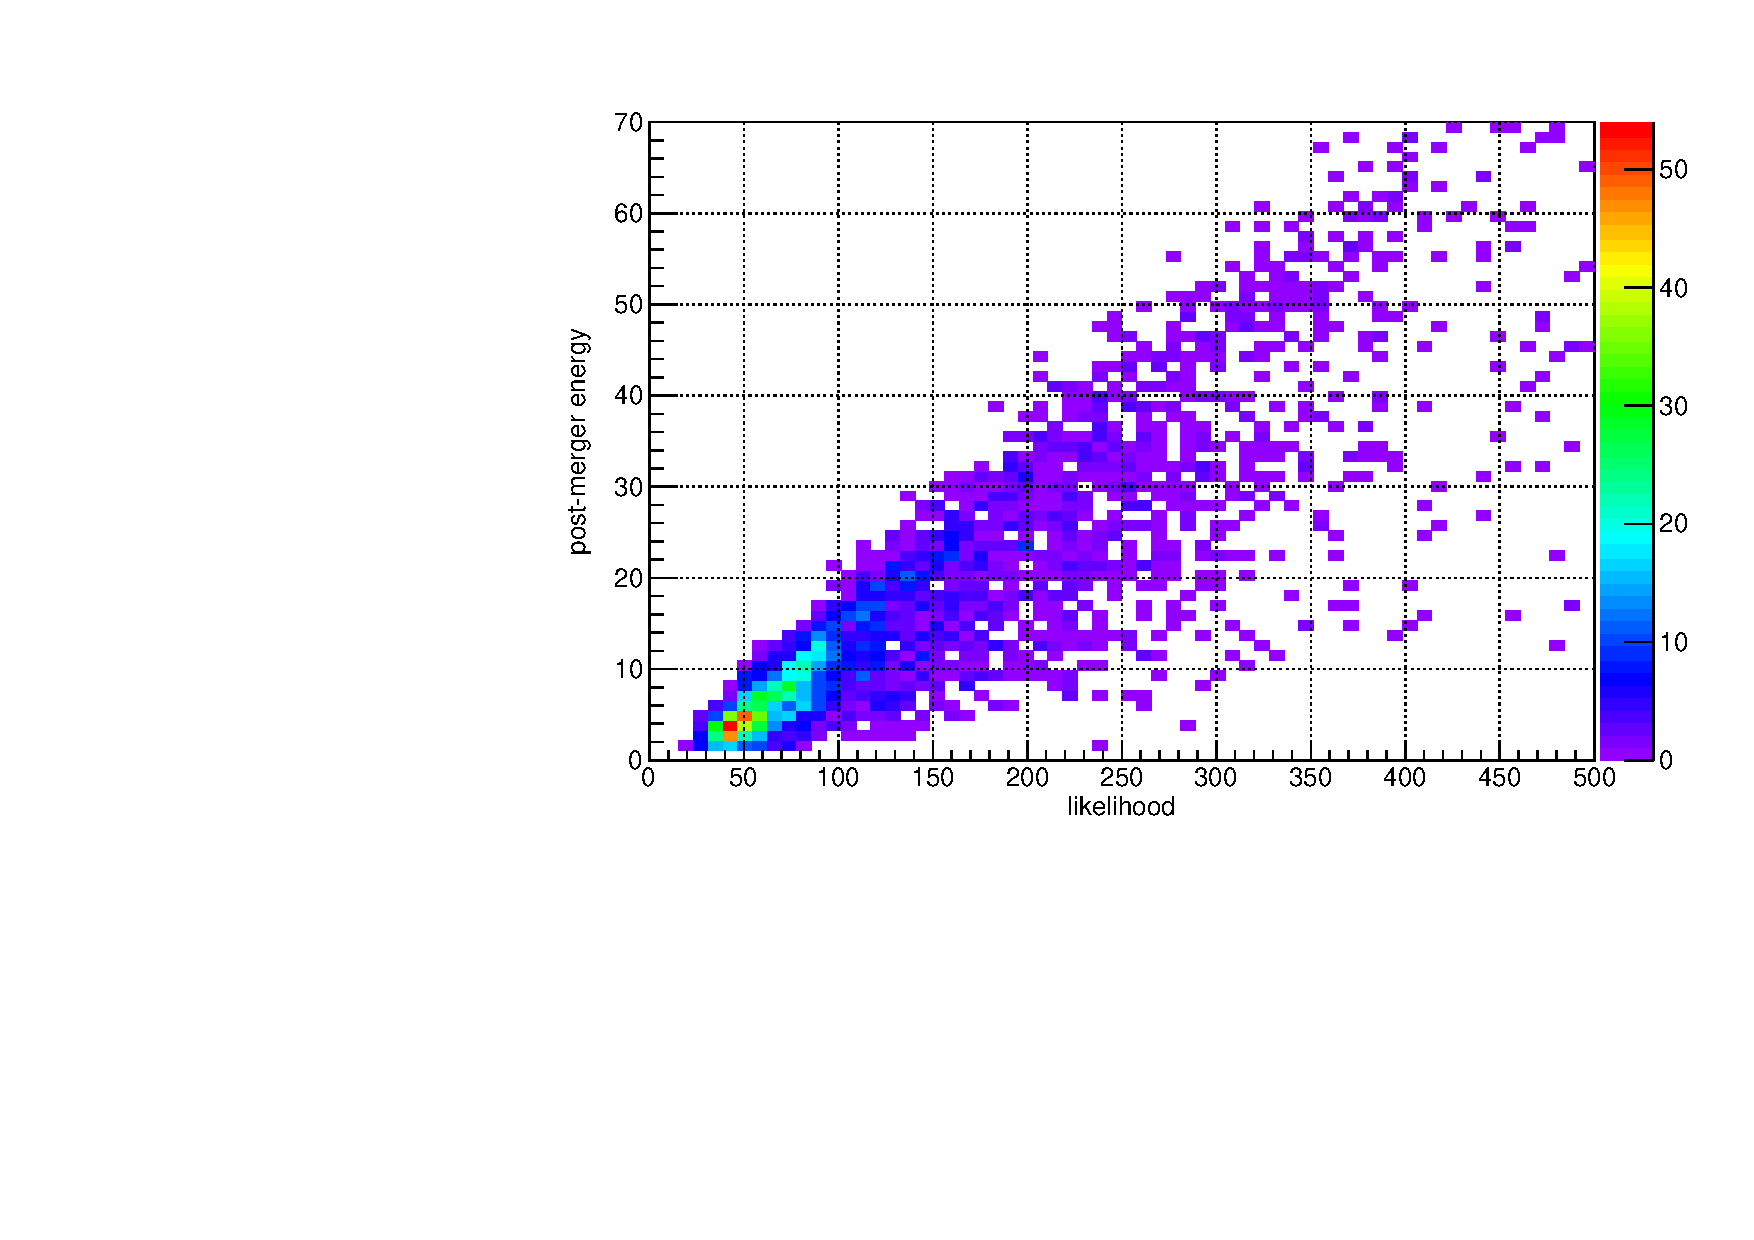
\includegraphics[width=.33333333333\textwidth]{figures/Capitolo_3/report/Likelihood_DistributionDetector1SHT2_0spin11.pdf}}
%	\subfloat[][\emph{SHT2\_2}]
%	{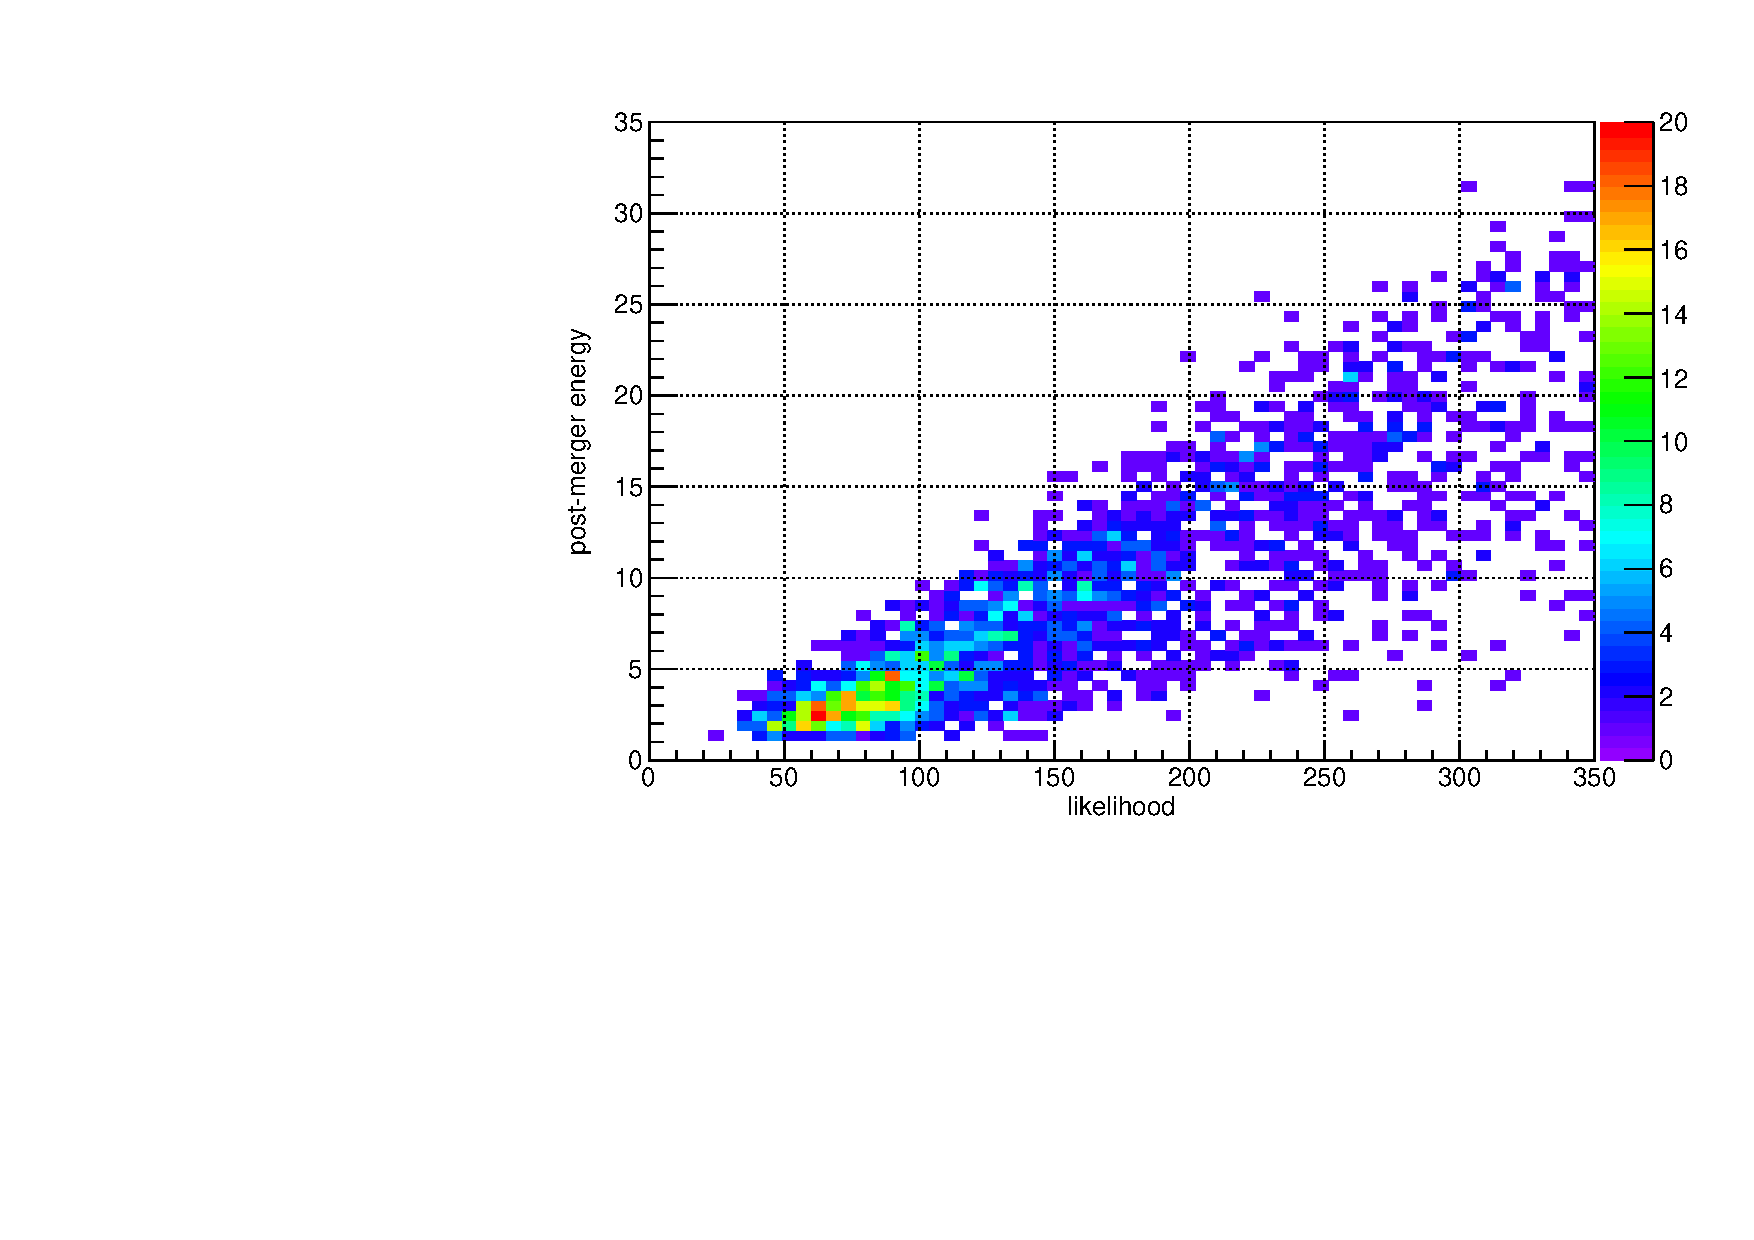
\includegraphics[width=.33333333333\textwidth]{figures/Capitolo_3/report/Likelihood_DistributionDetector1SHT2_2spin11.pdf}}
%	\subfloat[][\emph{APR4}]
%	{\includegraphics[width=.33333333333\textwidth]{figures/Capitolo_3/report/Likelihood_DistributionDetector1APR4_q091.pdf}}\\
%	\caption{Distribuzione delle energie della post coalescenza in funzione della verosimiglianza dell'evento, per LIGO Livingstone}
%	\label{fig:likelihood}
%\end{figure}